\documentclass[10pt]{book}

\usepackage{import}

% Searches packages and includes within docstyleDE relative to the given path "../"
\subimport{../}{docstyleDE}
% Important: the files docstyleDE.tex and ifiseries.sty must be in the same directory.

%\bibliographystyle{ksfh_nat}

\hypersetup{pdftitle=Simulation eines Vielkörpersystems auf einem verteilten Rechner}
\hypersetup{pdfauthor=Adrian Pegler}
\hypersetup{pdfsubject=Masterarbeit}
\hypersetup{pdfkeywords=}

\begin{document}
\frontmatter
  \thesistitlepage
    {Simulation eines Vielkörpersystems auf einem verteilten Rechner}
    %{Meine Fake Bachelorarbeit \\[.1em]mit einem sehr sehr \\[.1em]sehr langen Titel}% Title
    {Masterarbeit}% Thesistype
    {Adrian Pegler}% Name
    {\today}% Date
    {Dipl.-Inf. Sven Christophersen} % additional advisors (add more than one with: name1 \\& name2 \\& name3

  \eidesstatt{}

  \chapter*{Zusammenfassung}
    \blindtext

  \tableofcontents{}
  %\listoffigures{}\listoftables{}\lstlistoflistings{}
  %\chapter*{List of Acronyms}
  %% List of acronyms

\mainmatter

%% the actual thesis
%% use \include{filename} and \includeonly{filename} to organize your thesis

%Chapter: Einleitung
\chapter{Einleitung}
\label{ch:einl}
  \section*{Vorbemerkungen}
    Ich verwende in diesem Dokument den nach Herrn Prof. Dr. H. Laue benannten \textit{Lauehaken}: Sei $n \in \N$, dann bezeichnet $\haken{n}$ die Menge $\{1, \dots ,n\}$.
    In Anlehnung an die Schreibweise $\N_0$ für die natürlichen Zahlen $\N \cap \{0\}$ bezeichnet $\nullhaken{n}$ die Menge $\{0, \dots , n\}$.
  \section{Motivation}
  \label{sec:mot}
    Angeblich soll Sir Isaac Newton durch das Fallen eines Apfels die grundlegende Idee gehabt haben, dass die Mechanik des Himmels und der Erde doch dieselbe sein 
    könnte \citep{memoirs}. Jeder Schüler hat von dieser Geschichte gehört - und ob sie nun wahr ist oder nicht, sein Gesetz der nicht-relativistischen Gravitation ist bis
    heute eine wichtige Formel in der Physik.
    
    Seien für zwei Körper die Massen $m_1$, $m_2$ und Positionen $x_1$, $x_2$ gegeben. Dann wirkt durch die Masse $m_2$ eine Kraft $f$ auf die Masse $m_1$, die sich durch 
    \begin{equation}
      f = \gamma m_1 m_2 \frac{x_2 - x_1}{\norm{x_2 - x_1}^3_2}
      \label{eq:simple_grav}
    \end{equation}
    ergibt \citep{newton}. Dabei ist $\gamma \approx 6{,}67408*10^{-11} m^3 kg^{-1} s^{-2}$ die Gravitationskonstante \citep{graviconst} und $\norm{\cdot}_2: \R^d \to \R^d$ die 
    euklidische Norm $z \mapsto \sqrt{ \sum_{i \in \haken{d}} |z|^2 }$. Im Weiteren werden die Position eines Körpers und der Körper assoziiert. 
    
    Diese Formel für zwei Körper auszurechnen, stellt zunächst kein Problem dar. Von größerem Interesse für die Wissenschaft sind aber Mehrkörperprobleme, also die gravitationellen 
    Wechselwirkungen zwischen einer Menge von Körpern. Seien im Folgenden also $n \in \N$ und eine Menge $\Omega$ von $n$ Körpern gegeben.
    Für $x \neq y \in \Omega$ und die zugehörigen Massen $m_x$ und $m_y$ wirkt mit \autoref{eq:simple_grav} durch den Körper $y$ eine Kraft 
    \begin{equation}
      f_{xy} = \gamma m_x m_y \frac{y - x}{\norm{y - x}^3_2}
      \label{eq:multi_grav}
    \end{equation}
    auf den Körper $x$. Will man nun die kumulative Kraft berechnen, die durch alle Körper aus $\Omega$ auf den Körper $x$ wirkt, muss folgende Gleichung gelöst werden:
    \begin{equation}
      f_x = \sum_{\substack{y \in \Omega \\ y \neq x}} \gamma m_x m_y \frac{y - x}{\norm{y - x}^3_2}
      \label{eq:sum_grav}
    \end{equation}
    \citep{wissrech}.
    Für die Simulation aller auftretenden Gravitationskräfte müssen also für alle $n$ Körper jeweils $(n-1)$ Therme berechnet werden. Das Problem hat also eine Komplexität von
    $\mathcal{O}(n^2)$.
    
    Problematisch wird dies, wenn man sich beispielsweise die Dimensionen unseres Sonnensystems vergegenwärtigt. Laut NASA\footnote{
    World Book at NASA [2007]: 
    https://web.archive.org/\-web/\-20090412172631/\-http://mynasa.nasa.gov/\-worldbook/\-galaxy\_worldbook.html\\
    Archivierte url: http://mynasa.nasa.gov/worldbook/galaxy\_worldbook.html vom 12. April 2009. Abgerufen am 1. Mai 2018.} besteht die Milchstraße aus etwa 100 Milliarden
    (also $10^{11}$) Sonnen. Um sämtliche gravitationelle Wechselwirkungen in unserer Galaxie zu berechnen, müssten also ungefähr $(10^{11})^2 = 10^{22}$ Terme gelöst werden. Geht man 
    davon aus, dass ein aktueller Prozessor nicht mehr als eine Milliarde Terme pro Sekunde ausrechnen kann, so benötigt er etwa $10^{13}$ Sekunden, also mehr als 300.000 Jahre für 
    einen einzigen Simulationsschritt. Ein Problem dieser Größenordnung könnte also nicht in annehmbarer Zeit gelöst werden. \citep{wissrech} 
    
    In dieser Arbeit wird ein zweigleisiger Ansatz am vorliegenden Beispiel vorgestellt, mit dessen Hilfe Probleme dieser Größen- und Komplexitätsklasse in den Griff zu bekommen sind.
    
  \section{Ziele}
%     \TODO{Der erste Schritt ist über Approximation die Komplexitätsklasse des Problems zu reduzieren. Reduktion auf O(n)}
    Der erste Teil des Ansatzes ist eine Reduktion der Komplexitätsklasse des Gravitationsproblems. \autoref{eq:multi_grav} definiert eine vollbesetzte Matrix. Es gibt Möglichkeiten, solche
    Matrizen speicherplatzsparend durch Matrizen mit deutlich niedrigerem Rang anzunähern. Eine dieser Möglichkeiten ist die Darstellung als hierarchische Matrix. Diese Technik soll genutzt
    werden, um das vorliegende Problem in linearer Komplexität bewältigen zu können.
    
%     \TODO{In einem weiteren Schritt wird der vorige Algorithmus zur Ausführung auf Parallel-Rechner-Systemen angepasst.}
    Dieser Ansatz alleine wird aber nicht ausreichen, um das vorliegende Problem ausreichend schnell zu lösen. Wir werden daher zusätzlich nach einer Möglichkeit suchen, den Algorithmus parallel
    von vielen Rechnern gleichzeitig lösen zu lassen. Wir werden dazu einen Algorithmus vorstellen, der dies bewerkstelligt, und zeigen, dass dieser die Arbeit optimal auf die beteiligten
    Prozesse aufteilen kann.
  
  \section{Aufbau}
    Im folgenden Kapitel werden die \nameref{chp:foundations} der Arbeit vorgestellt. Den Anfang bilden die \hyperref[sec:h2]{hierarchischen Matrizen}. Dazu werden zunächst allgemeine Möglichkeiten 
    vorgestellt, eine Matrix als hierarchische Matrix darzustellen. Im Anschluss werden einige Möglichkeiten der Optimierung dieser Darstellung vorgestellt, die uns schließlich zu den sogenannten 
    \nameref{sec:hquad} führen, welche wir für die Darstellung des Gravitationsproblems nutzen wollen.
    
    In \autoref{sec:parrech} wird eine Zusammenfassung der Entwicklung der Computer hin zu Parallelität gegeben. Außerdem werden kurz Herausforderungen im Zusammenhang mit parallel arbeitenden
    Algorithmen erläutert. Im Anschluss wird mit dem \hyperref[sec:mpm]{Message-Passing-Modell} ein Modell vorgestellt, mit dem parallele Algorithmen strukturiert und viele der 
    Herausforderungen umgangen werden können.
    
    \autoref{sec:mpi} widmet sich einer Bibliothek, die das \hyperref[sec:mpm]{Message-Passing-Modell} umsetzt: das \hyperref[sec:mpi]{Message-Passing-Interface}. Diese Bibliothek werden wir später
    nutzen, um unseren Algorithmus zu parallelisieren.
    
    In \autoref{chp:haupt} wird zunächst die \nameref{sec:ausgang} für unseren Ansatz vorgestellt, also ein nicht-optimierter, nicht-parallel arbeitender Algorithmus zur Berechnung der gravitationellen
    Wechselwirkungen. Dann werden wir uns in \autoref{sec:approxf} eine Variante anschauen, die die Struktur der \nameref{sec:hquad}nutzt, um die Berechnungen deutlich effektiver durchzuführen.
    Schließlich wird in \autoref{sec:parallelpart} dieser Algorithmus noch um Möglichkeiten der Parallelisierung erweitert.
    
    Der erarbeitete Algorithmus muss natürlich noch \hyperref[chp:eval]{evalutiert} werden. In \autoref{chp:eval} werden wir zunächst eine \hyperref[sec:theo]{theoretische Abschätzung} der 
    Komplexitätsklasse des parallel arbeitenden Algorithmus vornehmen. Im Anschluss werden die theoretischen Überlegungen durch \nameref{sec:lauf} überprüft. 
    Den Abschluss bilden \nameref{chp:Conclusions}. 

\chapter{Grundlagen}
  \label{chp:foundations}
  \section{Hierarchische Matrizen}
  \label{sec:h2}
  Erinnern wir uns an \autoref{eq:multi_grav} aus der \nameref{ch:einl}, in welcher die gravitationelle Wechselwirkung zwischenzwei Körpern $x$ und $y$ beschrieben wurde. 
Die Struktur dieser Formel erinnert stark an Matrizen. 
Ein Ansatz, um große vollbesetzte Matrizen speicherplatzsparend aufzustellen und Berechnungen zeiteffektiv durchzuführen, besteht darin, sie als hierarchische Matrizen darzustellen.
Im Folgenden sollen daher die Grundlagen für allgemeine $\mathcal{H}$- und \hquad eingeführt werden. Für ausführlichere Arbeiten zu dem Thema der hierarchischen Matrizen verweise 
ich auf \citet{h2diss} und \citet{hackbusch1999sparse}.

\TODO{Quellenangaben einfügen: vgl. Nicht lokale Operationen}

Erarbeitet wurde das Konzept der hierarchischen Matrizen unter anderem zur effektiven Lösung Fredholmscher Integralgleichungen:
\begin{equation*}
  u\left(x\right) = \int_{\Omega} u\left(x\right) g\left(x, y\right) \forall x \in \Omega .
\end{equation*}
Dabei ist $\Omega \subseteq \R^d$ und $g \colon \R^d \times \R^d \to \R$ eine sogenannte \textit{Kernfunktion}.
Diskretisiert man diese Gleichung mit dem Galerkinverfahren unter Verwendung einer Finite-Elemente-Basis $\left(\phi_i\right)_{i \in I}$ erhält man die zugehörige Matrix
\begin{equation*}
  G_{ij} = \int_{\Omega} \int_{\Omega} \phi_i\left(x\right) g\left(x,y\right) \phi_j\left(y\right) \ dy \ dx ,\quad \forall i, j \in I.
\end{equation*} 
Um die Integration über $\Omega \times \Omega$ aufspalten zu können, ist es notwendig, dass die Variablen in der Kernfunktion getrennt werden können.
Die Kernfunktion $g$ muss also in der Form
\begin{equation*}
  g\left(x,y\right) = \sum_{\nu \in \haken{k}} a_{\nu}\left(x\right) b_{\nu}\left(y\right)
\end{equation*}
mit $k \in \N$, $a_{\nu}, b_{\nu} \colon \R^d \to \R$ vorliegt. Eine Kernfunktion dieser Form heißt \textit{entartete Kernfunktion} von Rang k.
Allgemein nennen wir eine Funktion $g$ eine Kernfunktion einer Matrix $G$, falls die Funktion $g$ die Matrix $G$ erzeugt, also gerade $G_{\mu\nu} = g{\mu, \nu}$ gilt.
Nicht jede Kernfunktion ist entartet, es lassen sich aber oft entartete Kernfunktionen konstruieren, die die Funktion approximieren. Möglichkeiten sind beispielsweise
Approximationen durch Taylor-Entwicklung oder Interpolation. \citep{h2diss}

Seien $X, Y$ Mengen und $G \in \R^{X \times Y}$ eine Matrix mit Kernfunkion $g \colon X \times Y \to \R$. Ist $g$ entartet, so gilt also für $x \in X$ und $y \in Y$ 
gerade $G_{xy} = g\left(x, y\right) = \sum_{\nu \in \haken{k}} a_{\nu}\left(x\right) b_{\nu}\left(y\right)$. Die Summe in dieser Gleichung können wir auch durch Multiplikation zweier Matrizen $A \in \R^{X \times k}$ und 
$\trans{B} \in \R^{Y \times k}$ mit $A_{x\nu} = a_{\nu}\left(x\right)$, $B_{y\nu} = b_{\nu}\left(y\right)$ ausdrücken. Analog dazu, die Kernfunktion als entartete Kernfunktion darzustellen, ist also die Darstellung der Matrix
$G$ durch Matrizen $A$ und $B$ durch $G = A\trans{B}$.
    
    \subsubsection{Approximation}
    \label{sec:approx}
      Im Folgenden möchte ich eine beispielhafte Approximation einer nicht-entarteten Kernfunktion durch Interpolation vorstellen, um so eine entartete Kernfunktion zu erhalten.
      Der Aufbau folgt weitestgehend dem von \citet{nichtlokop}. Für eine Approximation einer nicht-entarten Kernfunktion durch Taylor-Entwicklung verweise ich auf \citet{h2diss}. 
      
      Sei $g \colon \Omega \times \Omega \to \R$ eine nicht-entartete Kernfunktion. Für eine Interpolationsordnung $k$ und ein Teilgebiet $\sigma \subset \Omega$ wählen wir Interpolationspunkte 
      $\xi_\inds{1}, \dots , \xi_\inds{k}$. Nun suchen wir eine Approximation von $\left. g\right|_{\Omega \times \sigma}$ der Form
      \begin{equation}
      \label{eq:gsigma}
	g_\sigma\left(x, y\right) = \sum_{\nu \in \haken{k}} g\left(x, \xi_\inds{\nu}\right) \lag_\inds{\nu}\left(y\right),
      \end{equation}
      in der $x$ und $y$ getrennt sind. Somit hätten wir bereits eine entartete Kernfunktion. In eben dieser Form werden Lagrange-Interpolaten in Stützstellen 
      $\xi_\inds{\nu}$ mit Lagrange-Basisfunktionen $\lag_\inds{\nu}$ dargestellt. 
      
    \subsubsection{Lagrange-Interpolation im mehrdimensionalen Raum}
      Bevor wir die Funktion $g$ wie in \autoref{eq:gsigma} approximieren können, müssen wir die Lagrange-Basisfunktionen auf mehrdimensionalen Gebieten konstruieren und einige 
      Eigenschaften sicherstellen. 
      Zunächst definieren wir dazu die Lagrange-Basispolynome auf dem Referenzintervall $[-1,1]$. Für $k \in \N$, $\nu \in \nullhaken{k}$ und paarweise verschiedene Stützstellen
      $\xi_0, \dots , \xi_k \in [-1,1]$ ist durch
      \begin{equation*}
	\lag_\nu\left(x\right) := \prod_{\substack{\mu \in \nullhaken{k} \\ \mu \neq \nu}} \frac{x - \xi_\mu}{\xi_\nu - \xi_\mu} \ \ \ \ \ \ \ \ \ \ \ \  \text{für alle } x \in [-1,1]
      \end{equation*}
      das $\nu$-te Lagrange-Polynom gegeben.
      Eine Eigenschaft der Lagrange-Polynome, die wir später noch benötigen, ist:
      \begin{equation}
	\lag_\nu\left(\xi_\mu\right) = \delta_{\nu\mu} =
	\begin{cases}
	  1 & \text{falls } \nu = \mu,\\
	  0 & \text{sonst.}
	\end{cases}
	\label{eq:lag_delta}
      \end{equation}
      
      Wir können durch
      \begin{equation*}
	\mathfrak{I} \colon C[-1,1] \to \Pi_k, \ \ \ \ \ \ \ \ \ \ \ \ f \mapsto \sum_{\nu \in \nullhaken{k}} f\left(\xi_\nu\right) \lag_\nu
      \end{equation*}
      einen Lagrange-Interpolationsoperator definieren, der auf $[-1,1]$ stetige Funktionen auf Polynome aus $\Pi_k$ abbildet, also auf Polynome von höchstens Grad $k$.
      
      Um diesen Operator auf Funktionen auf beliebigen Intervallen $[a,b]$ mit $a < b$ zu übertragen, definieren wir eine Transformation
      \begin{equation*}
	\Phi_{[a,b]} \colon [-1,1] \to [a,b] \ \ \ \ \ \ \ \ \ \ \ \  x \mapsto \frac{b + a}{2} + \frac{b - a}{2} x,
      \end{equation*}
      die für alle $x \in [-1,1]$ die Eigenschaften
      \begin{equation*}
	\Phi_{[a,b]}\left(-1\right) = a , \ \ \ \ \Phi_{[a,b]}\left(1\right) = b , \ \ \ \ \Phi'_{[a,b]}\left(x\right) = \frac{b - a}{2} > 0
      \end{equation*}
      hat, also affin und bijektiv ist. Für $f \in C[a,b]$ gilt also $\tilde f := f \after \Phi_{[a,b]} \in C[-1,1]$, sodass wir den auf $[-1,1]$ definierten Interpolationsoperator $\mathfrak{I}$
      auf $\tilde f$ anwenden können. Wir können also einen Interpolationsoperator auf dem Intervall $[a,b]$ durch
      \begin{equation*}
	\mathfrak{I}_{[a,b]} \colon C[a,b] \to \Pi_k, \ \ \ \ \ \ \ \ \ \ \ \ f \mapsto \mathfrak{I}[f \after \Phi_{[a,b]}] \after \Phi_{[a,b]}^{-1}
      \end{equation*}
      definieren, was, die Definition von $\mathfrak{I}$ eingesetzt, die Darstellung
      \begin{equation*}
	\mathfrak{I}_{[a,b]}[f] = \sum_{\nu \in \nullhaken{k}} f \after \Phi_{[a,b]}\left(\xi_\nu\right) \lag_\nu \after \Phi_{[a,b]}^{-1} = 
				 \sum_{\nu \in \nullhaken{k}} f \left( \Phi_{[a,b]}\left(\xi_\nu\right)\right)     \lag_\nu \after \Phi_{[a,b]}^{-1}
      \end{equation*}
      ergibt.
      
      Zur Vereinfachung definieren wir für $\nu \in \nullhaken{k}$ und $x \in [a,b]$
      \begin{align*}
	\xi_{[a,b],  \nu} &:= \Phi_{[a,b]}\left(\xi_\nu\right) = \frac{b + a}{2} + \frac{b - a}{2} \xi_\nu\\
	\lag_{[a,b], \nu} &:= \prod_{\substack{\mu \in \nullhaken{k} \\ \mu \neq \nu}} \frac{x - \xi_{[a,b],  \mu}}{\xi_{[a,b],  \nu} - \xi_{[a,b],  \mu}}.
      \end{align*}
      Da mit \autoref{eq:lag_delta} folgende Gleichung für alle $\nu,\mu \in \nullhaken{k}$ gilt
      \begin{align*}
	 \lag_\nu \after \Phi_{[a,b]}^{-1}\left(\xi_{[a,b],\mu}\right) &= \lag_\nu \after \Phi_{[a,b]}^{-1} \left( \Phi_{[a,b]}\left(\xi_{[a,b],\mu}\right) \right)\\
							    &= \lag_\nu \left(\xi_\mu\right) = \delta_{\nu\mu}\\
							    &= \lag_{[a,b],\nu}\left( \xi_{[a,b],\mu} \right),
      \end{align*}
      stimmen $\lag_\nu \after \Phi_{[a,b]}^{-1}$ und $\lag_{[a,b],\nu}$ in $k+1$ Punkten überein. Da beides Polynome in $\Pi_k$ sind, müssen sie identisch sein und wir erhalten die vereinfachte
      Darstellung
      \begin{equation*}
	\mathfrak{I}_{[a,b]}[f] = \sum_{\nu \in \nullhaken{k}} f\left(\xi_{[a,b],\nu}\right) \lag_{[a,b],\nu}, \ \ \ \ \ \ \ \ \ \ \ \ \text{für alle } f \in C[a,b].
      \end{equation*}
      
      
      Nun müssen wir für unser Problem noch Interpolationsoperatoren auf Gebieten im mehrdimensionalen Raum definieren. Der Einfachheit halber, und weil der später vorgestellte Algorithmus ohnehin 
      mit solchen sogenannten \wlabel{\textit{bounding boxes}}{w:bbox} arbeitet, beschränken wir uns auf achsenparallele Quader $Q = [a_1,b_1] \times \dots \times [a_d,b_d]$. Sei also eine zu interpolierende Funktion
      $f \in C\left(Q\right)$ gegeben. Für $\iota \in \haken{d}$ und $x \in Q$ gewinnen wir aus $f$ eine Funktion
      \begin{equation*}
	f_{x,\iota} \colon [a_\iota,b\iota] \to \R, \ \ \ \ \ \ \ \ \ \ \ \ y \mapsto f\left(x_1, \dots , x_{\iota-1}, y , x_{\iota+1}, \dots , x_d\right),
      \end{equation*}
      bei der alle Parameter außer dem $\iota$-ten fest sind. Auf diese Funktion auf dem Intervall $[a_\iota,b_\iota]$ können wir den Interpolationsoperator $\mathfrak{I}_{[a_\iota,b_\iota]}$ 
      anwenden und erhalten so einen Operator
      \begin{equation*}
	\mathfrak{I}_{Q,\iota} \colon C\left(Q\right) \to C\left(Q\right)
      \end{equation*}
      für den für $f \in C\left(Q\right)$ und $x \in Q$
      \begin{equation*}
	\mathfrak{I}_{Q,\iota}[f]\left(x\right) = \sum_{\nu \in \nullhaken{k}} f\left(x_1, \dots , x_{\iota-1} , \xi_{[a_\iota,b_\iota]} , x_{\iota+1}, \dots , x_d\right) \lag_{[a_\iota,b_\iota],\nu}\left(x_\iota\right)
      \end{equation*}
      gilt.
      Somit bildet $\mathfrak{I}_{Q,\iota}$ eine stetige Funktion auf eine neue stetige Funktion ab, die sich in der $\iota$-ten Komponente wie ein Polynom verhält. Durch Hintereinanderausführung
      der Operatoren für jede Dimension erhalten wir ein Polynom in jeder Komponente und mit
      \begin{equation*}
	\mathfrak{I}_Q := \mathfrak{I}_{Q,1} \after \dots \after \mathfrak{I}_{Q,d}
      \end{equation*}
      einen Interpolationsoperator, der für alle $f \in C\left(Q\right)$ und $x \in Q$ die Gleichung
      \begin{equation*}
	\mathfrak{I}_Q[f]\left(x\right) = \sum_{\nu_1 \in \nullhaken{k}} \dots \sum_{\nu_d \in \nullhaken{k}} 
			      f \left( \xi_{[a_1,b_1],\nu_1}, \dots , \xi_{[a_d,b_d],\nu_d} \right) 
			      \lag_{[a_1,b_1],\nu_1}\left(x_1\right) \dots  \lag_{[a_d,b_d],\nu_d}\left(x_d\right)
      \end{equation*}
      erfüllt. Mit den Definitionen
      \begin{align*}
	\xi_{Q ,\nu} &= \left(\xi_{[a_1,b_1],\nu_1} ,    \dots , \xi_{[a_d,b_d],\nu_d}\right),\\
	\lag_{Q,\nu} &= \lag_{[a_1,b_1],\nu_1}\left(x_1\right) \dots  \lag_{[a_d,b_d],\nu_d}\left(x_d\right) \text{, für alle } \nu \in M := \nullhaken{k}^d, \ x \in Q
      \end{align*}
      erhalten wir die gewohnte Darstellung
      \begin{equation*}
	\mathfrak{I}_Q[f] = \sum_{\nu \in M} f\left(\xi_{Q,\nu}\right)\lag_{Q,\nu} \text{, für alle } f \in C\left(Q\right).
      \end{equation*}
      
      Mit diesem Interpolationsoperator können wir nun die entartete Approximation der Kernfunktion $g$ aus \autoref{eq:gsigma} konstruieren. Dazu identifizieren wir $\sigma \in T_\Omega$
      mit einem überdeckenden Quader $Q_\sigma$.
    
    \subsubsection{Zulässigkeit}
    \label{sec:zul}
      Wir haben also über Interpolation eine entartete Kernfunktion $g_\sigma$ konstruiert. Für $x \in \Omega$ und $y \in \sigma$ approximiert die Funktion $g_\sigma$ die Funktion $g$ allerdings 
      nur dann gut, wenn $x$ und $\sigma$ hinreichend weit voneinander entfernt sind (vgl. \citet{h2diss, nichtlokop}). 
      Daher wollen wir nun eine Bedingung einführen, die eine Aussage darüber trifft, ob das Gebiet $\sigma$ für ein Gebiet $\tau$ zulässig, also für alle $x \in \tau$
      hinreichend weit entfernt ist. Das Gebiet $\tau$ wird auch \textit{Target-} oder \textit{Zielgebiet}, das Gebiet $\sigma$ auch \textit{Source-} oder \textit{Quellgebiet} genannt.
      %Weiterhin kann die Güte der Approximation durch die Anzahl und Art der Interpolationspunkte verändert werden.
      
      \begin{defn}
	(Zulässigkeitsbedingung)\\
	Wir nennen eine Abbildung, die jedem Paar $\left(\tau, \sigma\right) \in \pot{\Omega} \times \pot{\Omega}$ entweder \textit{``zulässig''} oder \textit{``unzulässig''} zuordnet, 
	\textit{Zulässigkeitsbedingung}.       
      \end{defn}
      
      Für eine konkrete Zulässigkeitsbedingung benötigen wir noch ein paar Definitionen.
            
      Seien $\sigma, \tau \subseteq \Omega$. Dann bezeichnet
      \begin{equation*}
	diam\left(\sigma\right) := max\{ \norm{x-y} \ | \ x, y \in \sigma \}
      \end{equation*}
      den Durchmesser eines Teilgebiets und
      \begin{equation*}
	dist\left(\sigma, \tau\right) := min\{ \norm{x-y} \ | \ x \in \sigma, y \in \tau \}
      \end{equation*}
      den Abstand der beiden Teilgebiete zueinander. 
      
      Damit lässt sich die von \citet{h2diss} aufgeführte $\eta$-Zuläs\-sig\-keit wie folgt definieren:
      
      \begin{defn}
	($\eta$-Zulässigkeit)\\
	Sei $\eta \in \R^{+}$. Dann heißt die Abbildung $\mathcal{Z}_\eta \colon \pot{\Omega} \times \pot{\Omega} \to \{\ttit{zulässig},\ttit{unzulässig}\}$ mit 
	\begin{equation*}
	  \mathcal{Z}_\eta \left( \tau, \sigma \right) = 
	  \begin{cases}
	    \ttit{zulässig}   & \text{falls }\{diam\left(\tau \right), diam\left( \sigma \right)\} \le 2 \eta dist\left( \tau , \sigma \right)\\
	    \ttit{unzulässig} & \text{sonst}
	  \end{cases}
	\end{equation*}
	\textit{$\eta$-Zulässigkeitsbedingung}. Paare $\left(\tau, \sigma\right)$, für die $\mathcal{Z}\left(\tau, \sigma\right) = \ttit{zulässig}$ gilt, werden \textit{$\eta$-zulässig} genannt.
      \end{defn}

      Für kleine $\eta$ zeigen \citet{h2approxint} die exponentielle Konvergenz der durch Interpolation approximierten Funktion gegen die Kernfunktion und \citet{h2diss} die exponentielle Konvergenz
      bei Approximation durch Taylor-Entwicklung.
      
      \citet{nichtlokop} weist nach, das für asymptotisch glatte Funktionen die Approximation für jedes $\eta > 0$ exponentiell konvergiert, wenn die obige Zulässigkeitsbedingung erfüllt ist.
      Eine unendlich oft differenzierbare Kernfunktion $g$ heißt asymptotisch glatt, wenn für alle $\alpha , \beta \in \N_0^d$, $x , y \in \R^d$, $x \neq y$, Konstanten $C \colon \N^2 \to \R_{> 0}$
      existieren, sodass die partiellen Ableitungen von $g$ wie folgt abgeschätzt werden können:
      \begin{equation*}
	|\partial_x^\alpha \partial_y^\beta g\left(x,y\right)| \leq C\left( |\alpha| , |\beta| \right) \norm{ x - y }^{-|\alpha| -|\beta|} | g\left( x,y \right) |.
      \end{equation*}
      (vgl. \citet{h2approxint})
      
    \subsubsection{Tschebyscheff-Interpolationspunkte}
    \label{sec:tscheby}
      Die Wahl der Zulässigkeitsbedingung ist nicht der einzige Einflussfaktor auf die Genauigkeit der Approximation. Auch die Wahl der Interpolationspunkte trägt dazu bei.
      Als optimale Interpolationspunkte haben sich die Tschebyscheff-Interpolationspunkte erwiesen (vgl. \citet{nichtlokop}). Daher führen wir diese im Folgenden kurz ein.
      
      \begin{defn}
	(Tschebyscheff-Polynome)\\
	Durch
	\begin{equation*}
	  T_n = 
	  \begin{cases}
	    1  				& \text{ falls } n = 0\\
	    x				& \text{ falls } n = 1\\
	    2 x T_{n-1}\left(x\right) - T_{n-2}\left(x\right) & \text{ sonst,}
	  \end{cases}
	  \ \ \ \ \ \ \ \ \ \ \ \ \text{für alle } n \in \N_0, \ x \in \R
	\end{equation*}
	wird eine Familie $\left(T_n\right)_{n \in \N_0}$ von Polynomen definiert. Für $n \in \N_0$ bezeichnen wir $T_n$ als $n$-tes Tschebyscheff-Polynom.
	\citep{nichtlokop}
      \end{defn}
      
      Mit Hilfe des Additionstheorems $\cos \left(\alpha + \beta\right) = \cos \alpha \cos \beta - \sin \alpha \sin \beta$ und den Eigenschaften des Cosinus lässt sich leicht die folgende Aussage zeigen.
      
      \begin{lemdef}
	Für $n \in \N_0$ und $x \in [-1,1]$ gilt:
	\[
	  T_n\left(x\right) = \cos \left( n \arccos \left(x\right) \right).
	\]
	Daraus folgen insbesondere die $n$ reellen einfachen Nullstellen
	\[
	  T_n\left( \xi_\nu \right) = 0, \ \ \ \ \ \ \ \ \ \ \ \ \xi_\nu := \cos \left(\pi \frac{2\nu + 1}{2n} -\right) \ \ \ \ \ \ \ \ \ \ \ \ \text{für alle } \nu \in \haken{n}.
	\]
	Diese Nullstellen nennen wir \textit{Tschebyscheff-Interpolationspunkte}.
	\citep{nichtlokop}
      \end{lemdef}
      
    \subsubsection{Clusterung}
    \label{sec:cluster}
      Im Abschnitt \nameref{sec:approx} wurde gezeigt, wie die Kernfunktion auf Teilgebieten approximiert werden kann, sofern die Paare von Gebieten zulässig sind.
      Im Abschnitt \nameref{sec:zul} wurde eine Bedingung aufgestellt, wann Paare von Gebieten zulässig sind und wann nicht.
      In diesem Kapitel soll eine Struktur vorgestellt werden, mit der solche Paare von Teilgebieten strukturiert werden können.
      Dazu werden zunächst einige grundlegende Definitionen benötigt.
      
      \begin{defn}
      \label{def:tree}
	(Baum)\\
	Ein Paar $T = \left(V,E\right)$ mit $E \subset V \times V$ nennen wir einen Baum mit Knoten $V$ und Kanten $E$, wenn die folgenden Bedingungen erfüllt sind:
	\begin{enumerate}
	  \item Es gibt genau ein Element $root\left(T\right) \in V$, so dass für alle $v \in V$ gilt $\left(v, root\left(T\right)\right) \notin E$. Dieses Element heißt \textit{Wurzel} des Baumes T.
	  \item Zu jedem Knoten $v \in V \backslash \{root\left(T\right)\}$ gibt es $n \in \N$ und einen Weg $\left(v_i\right)_{i = 0}^n$ der Länge $n$ von der Wurzel $root\left(t\right) = v_0$ zu dem Knoten
		$v = v_n$ mit $\left(v_{i-1}, v_{i}\right) \in E$ für $i \in \haken{n}$.
	  \item Es gibt keine Zyklen.
	\end{enumerate}
	Es gelten folgende Notationen:
	\begin{enumerate}
	  \item Die Länge des längsten Weges in $T$ heißt die \textit{Tiefe} des Baumes und wird mit $depth\left(T\right)$ bezeichnet.
	  \item Mit $``q \in T''$ ist stets $``q \in V''$ gemeint.
	  \item $sons\left(q\right) := sons_T\left(q\right) := \{v \in V \ | \ \left(q,v\right) \in E\}$ ist die Menge der \textit{Söhne} eines Knotens $q \in T$.
	  \item $sons^*\left(q\right) := 
	    \begin{cases}
	      {q} \cup \bigcup_{\tilde q \in sons(q)} sons^*\left( \tilde q \right) & \text{falls } sons(t) \neq \emptyset,\\
	      {q} 								   & \text{sonst,}
	    \end{cases}$
	    ist die Menge aller Nachfahren eines Knotens $q \in T$.
	  \item $T^{\left(i\right)}$ bezeichnet die $i$-te Ebene des Baumes. Dabei gilt:
	    \begin{enumerate}
	      \item $T^{\left(0\right)} := \{root\left(T\right)\}$ und
	      \item $T^{\left(i\right)} := \{\tilde v \in V \ | \ \exists v \in T^{\left(i-1\right)} \colon \tilde v \in sons\left(v\right)\}$ für $i \in \haken{depth\left(T\right)}$.
	    \end{enumerate}
	  \item Der Begriff ``oberhalb'' bedeutet ``näher zur Wurzel'', der Begriff ``unterhalb'' respektive ``weiter oder gleich weit entfernt von der Wurzel''.
	  \item $\mathcal{L}\left(T\right) := \{q \in T \ | \ \forall v \in T \colon \left(q,v\right) \notin E \}$ bezeichnet die Menge aller Blätter des Baumes T.
	  \item $\mathcal{L}\left(T,i\right) := \mathcal{L}\left(T\right) \cap T^{\left(i\right)}$ ist die Menge der Blätter auf der $i$-ten Ebene des Baumes.
	  \item $\mathcal{L}\left(T,\leq s\right) := \mathcal{L}\left(T\right) \cap \bigcup_{i \in \nullhaken{s}} T^{\left(i\right)}$ sind alle Blätter der Ebenen $0, \dots ,s \leq depth\left(T\right)$.
	\end{enumerate}
	\nopagebreak[4]
	\citep{h2diss}
      \end{defn}
      
      Mit Hilfe einer Baumstruktur wollen wir nun eine Struktur definieren, mit der im Allgemeinen eine beliebige Menge $M$ hierarchisch partitioniert werden kann. Diese Struktur wollen
      wir dann für unsere Menge $\Omega$ nutzen.
      
      \begin{defn}
      \label{def:clusterbaum}
	(Clusterbaum)\\
	Wir nennen einen Baum $T = \left(V,E\right)$ mit $V \subseteq \pot{M} \backslash \{ \emptyset \}$ einen \textit{Clusterbaum} einer Menge $M$, falls die nachfolgenden 
	Bedingungen erfüllt sind:
	\begin{enumerate}
	  \item $root\left(T\right) = M$
	  \item $\forall t \in T : t = {\bigcup}_{s \, \in \, sons\left(t\right)} s.$
	  \item $\forall t \in T \ \forall s_0, s_1 \in sons\left(t\right) : s_0 \cap s1 = \emptyset$
	\end{enumerate}
	Für einen Clusterbaum verwenden wir in der Regel die Notation $T_M$ um auf die verwendete Indexmenge hinzuweisen, und bezeichnen die Knoten $t \in T_M$ als \textit{Cluster}.
	\citep{nichtlokop}
      \end{defn}
      
      \citet{h2diss} nennt Clusterbäume auch hierarchische Partitionsbäume oder kurz $\mathcal{H}$-Bäume der Menge $M$. Der Name leitet sich direkt von den Eigenschaften
      des Clusterbaumes her. Es gilt nämlich:
      \begin{enumerate}
      \item Die Menge $P_M^{\left(i\right)} := T_M^{\left(i\right)} \cup \mathcal{L}\left(T, \leq i\right)$ für bildet für alle $i \in \nullhaken{depth\left(T_M\right)}$ eine disjunkte Partition der Menge M.
      \item Die Partitionen sind über die Ebenen des Baumes hierarchisch angeordnet. Damit ist gemeint, dass für alle $i \in \haken{depth\left(T_M\right)}$ die Partition $P^{\left(i\right)}$ mehr Teilmengen beinnhaltet
	    als die Partition $P^{\left(i-1\right)}$.
      \end{enumerate}

      Mit Hilfe eines Clusterbaumes können Partitionen einer Menge also hierarchisch strukturiert werden. Meist werden sie genutzt, um eine Indexmenge oder
      die geometrische Struktur eines Problems zu partitionieren. Letztere Variante wird auch \textit{geometrischer Clusterbaum} genannt. 
      
      Ein weiterer praktischer Aspekt
      von Clusterbäumen ist ihre gute rekursive Konstruierbarkeit. Beginnend mit der vollständigen Menge $M$ wird ein Cluster jeweils in Sohncluster unterteilt,
      bis entweder in den Blättern jeweils nur noch ein Element vorhanden ist oder eine anders geartete Abbruchbedingung erfüllt ist. Für praktische Anwendungen ist
      es in der Regel nicht effizient, bis zu einelementigen Mengen zu teilen. Üblich sind Abbruchbedingungen, die eine gewisse Mächtigkeit für Blattmengen vorgeben.
      Wird diese unterschritten, wird nicht weiter geteilt. 
      
      Das Teilen der Cluster kann ebenfalls unterschiedlich motiviert sein. Naheliegend sind kardinalitätsgesteuerte Zerlegungen, um ein optimales Loadbalancing zu erhalten,
      sowie die Zerlegung anhand der zugrundeliegenden geometrischen Struktur. Auch kombinierte Zerlegungen sind denkbar.
      
      \begin{figure}[b]
	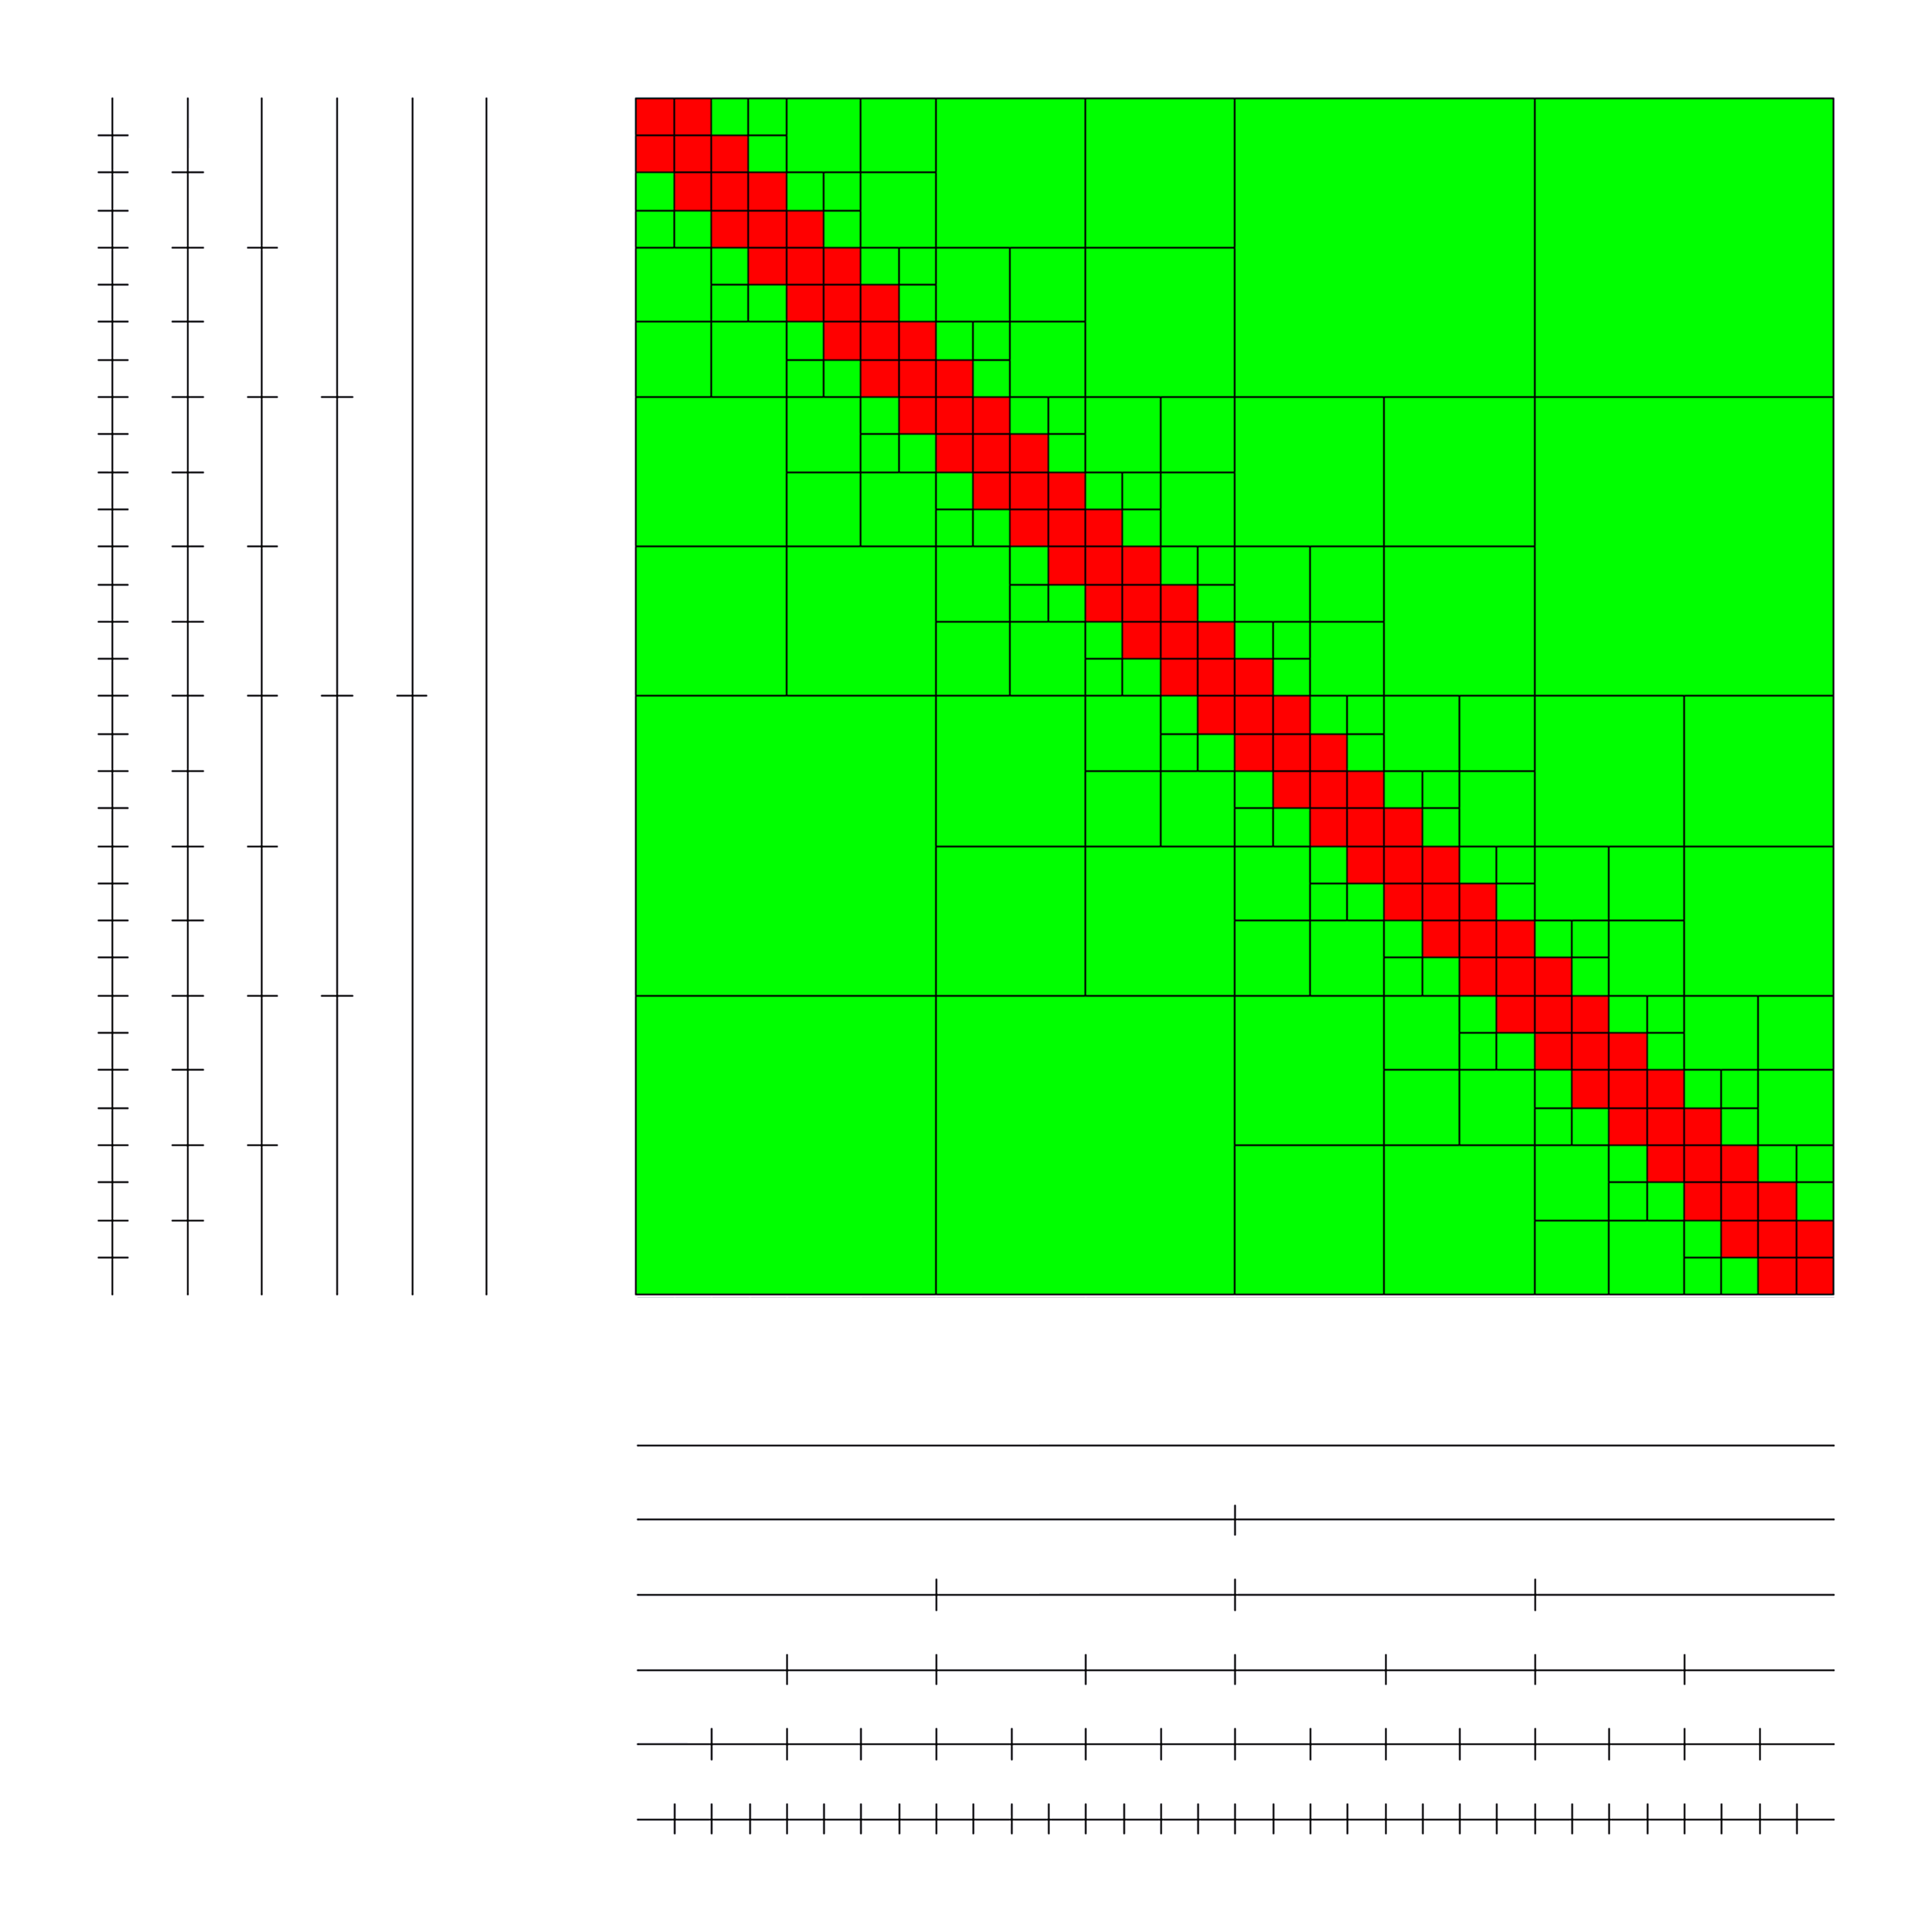
\includegraphics[width=0.68\textwidth]{img/blockbaum.png}
	\caption{Schematische Darstellung eines Blockbaumes. In grün sind zulässige, in rot unzulässige Blöcke gekennzeichnet. (Quelle: \citet{h2-slides})}
	\label{fig:blockbaum}
      \end{figure}
      
      \begin{defn}
	(Blockbaum, (streng) zulässiger Blockbaum)\\
	Seien Menge $X, Y$ und jeweils zugehörige Clusterbäume $T_X$ und $T_Y$ gegeben.
	
	Einen Clusterbaum $T_{X \times Y}$ der Menge $X \times Y$ mit folgenden Eigenschaften:
	\begin{enumerate}
	  \item Für alle Knoten $b \in T_{X \times Y}$ existieren Knoten $t \in T_X$ und $s \in T_Y$, sodass $b = t \times s$
	  \item Falls $b = t \times s \in T_{X \times Y}$ kein Blatt ist, gilt
	  \begin{equation*}
	    sons\left(b\right) = 
	    \begin{cases}
	      \{ t \times s'\ \,\ | \  s'\!\in sons\left(s\right) \} & \text{falls } sons\left(t\right) = \emptyset, \ sons\left(s\right) \neq \emptyset \\
	      \{ t' \times s\ \,\ | \  t'  \in sons\left(t\right) \} & \text{falls } sons\left(t\right) \neq \emptyset, \ sons\left(s\right) = \emptyset \\
	      \{ t' \times s' \:\ | \  t'  \in sons\left(t\right),\ s' \in sons\left(s\right) \} & \text{ansonsten}\\
	    \end{cases}
	  \end{equation*}
	\end{enumerate}
	nennen wir \textit{Blockbaum} und seine Knoten \textit{Blöcke}. Die Komponenten $t \in T_X$ und $s \in T_Y$ werden auch \textit{Zeilen-} und \textit{Spaltencluster}
	genannt.
	
	Wir nennen einen Block $b = t \times s$ \textit{zulässig} bezüglich einer Zulässigkeitsbedingung $\mathcal{Z}$, wenn $\mathcal{Z}\left(t,s\right) = \ttit{zulässig}$ erfüllt ist.
	
	Wir nennen einen Blockbaum zulässig, wenn für alle Blattblöcke $b = t \times s \in \mathcal{L}\left(T_{X \times Y}\right)$ gilt:
	\begin{equation*}
	  \mathcal{Z}\left(t,s\right) = \ttit{zulässig} \text{ oder }
	  sons\left(t\right) = \emptyset \text{ oder }
	  sons\left(s\right) = \emptyset.
	\end{equation*}      
	Wir nennen ihn \textit{streng zulässig}, wenn gilt:
	\begin{equation*}
	  \mathcal{Z}\left(t,s\right) = \ttit{zulässig} \text{ oder }
	  sons\left(t\right) = \emptyset = sons\left(s\right),
	\end{equation*}
	Mit
	\begin{align*}
		      \mathcal{L}^+\left(T_{X \times Y}\right) &= \{ b = t \times s \in  \mathcal{L}\left(T_{X \times Y}\right) \ | \ \mathcal{Z}\left(t,s\right) = \ttit{zulässig} \}\\
	  \text{und } \mathcal{L}^-\left(T_{X \times Y}\right) &= \{ b = t \times s \in  \mathcal{L}\left(T_{X \times Y}\right) \ | \ \mathcal{Z}\left(t,s\right) = \ttit{unzulässig} \}
	\end{align*}
	bezeichnen wir die Mengen der zulässigen beziehungsweise unzulässigen Blätter eines Blockbaumes. $\mathcal{L}^+\left(T_{X \times Y}\right)$ wird auch \textit{Fernfeld} und 
	$\mathcal{L}^-\left(T_{X \times Y}\right)$ \textit{Nahfeld} genannt. Die Namen leiten sich von der $\eta$-Zulässigkeitsbedingung her, die auf der relativen Nähe der Cluster zueinander beruht.
	
      \end{defn}

      
      Mit Hilfe von Blockbäumen können wir nun also Paare von Teilgebieten hierarchisch strukturieren und auf Zulässigkeit prüfen.
      In \autoref{fig:blockbaum} ist ein Blockbaum, beziehungsweise die Blätter eines Blockbaumes, dargestellt. Zulässige Blattblöcke sind grün, unzulässige rot gekennzeichnet. Zur linken
      den Blockbaumes ist der Clusterbaum mit den Targetclustern, unten der Clusterbaum mit den Sourceclustern schematisch abgebildet.
%       Damit haben wir nun alles Notwendige bei der Hand um \hmat definieren zu können.
      
  \subsection{\hmat}
  \label{sec:hmat}
    \begin{defn}
      (\Rk-Matrix)\\
      Seien $m,n,k \in \N$ sowie $M \in \R^{m \times n}$ gegeben. Wir nennen $M$ eine \textit{\Rk-Matrix}, wenn Matrizen $A \in \R^{m \times k}$ und $B \in \R^{n \times k}$  existieren, sodass
      \begin{equation*}
	M = A \trans{B}
      \end{equation*}
      gilt. Die Menge aller solcher \Rk-Matrizen bezeichnen wir mit
      \begin{equation*}
	\mathcal{R}\left(m,n,k\right) = \{M \in \R^{m \times n} \ | \ M = A\trans{B}, A \in \R^{m \times k}, B \in \R^{n \times k}\}.
      \end{equation*}
      \citep{nichtlokop}
    \end{defn}
    
    Das praktische an \Rk-Matrizen ist, dass sie sich durch $k\left(m+n\right)$ Koeffizienten darstellen lassen. Ist $k \ll m,n$ ist dies wesentlich effizienter als eine volle Darstellung mit $m \cdot n$ 
    Koeffizienten. \citep{nichtlokop}
    
    \begin{defn}
    \label{def:hmat}
      (Hierarchische Matrix oder $\mathcal{H}$-Matrix)\\
      Seien $X$, $Y$ zwei Mengen, $T$ ein zugehöriger zulässiger Blockbaum mit Zulässigkeitsbedingung $\mathcal{Z}$ und $k: \mathcal{L}\left(T\right) \to \N_0$ die Rangverteilung der Blätter.
      
      Eine Matrix $M \in \R^{X \times Y}$ heißt \textit{hierarchische Matrix} oder kurz \textit{$\mathcal{H}$-Matrix} bezüglich $T$, $\mathcal{Z}$ und $k$, falls für jeden Blattblock
      $b \in \mathcal{L}\left(T\right)$ der korrespondierende Matrixblock $M_b = \left(M_{ij}\right)_{\left(i,j\right) \in b}$ eine \Rk-Matrix ist.
      
      Eine Zahl $k_0 \in \N$ mit $k\left(b\right) \leq k_0$ für alle $b \in \mathcal{L}^+\left(T_{X \times Y}\right)$ heißt lokaler Rang der hierarchischen Matrix.
      
      \citep{h2diss, nichtlokop}
      
    \end{defn}
    
    \begin{figure}[t]
      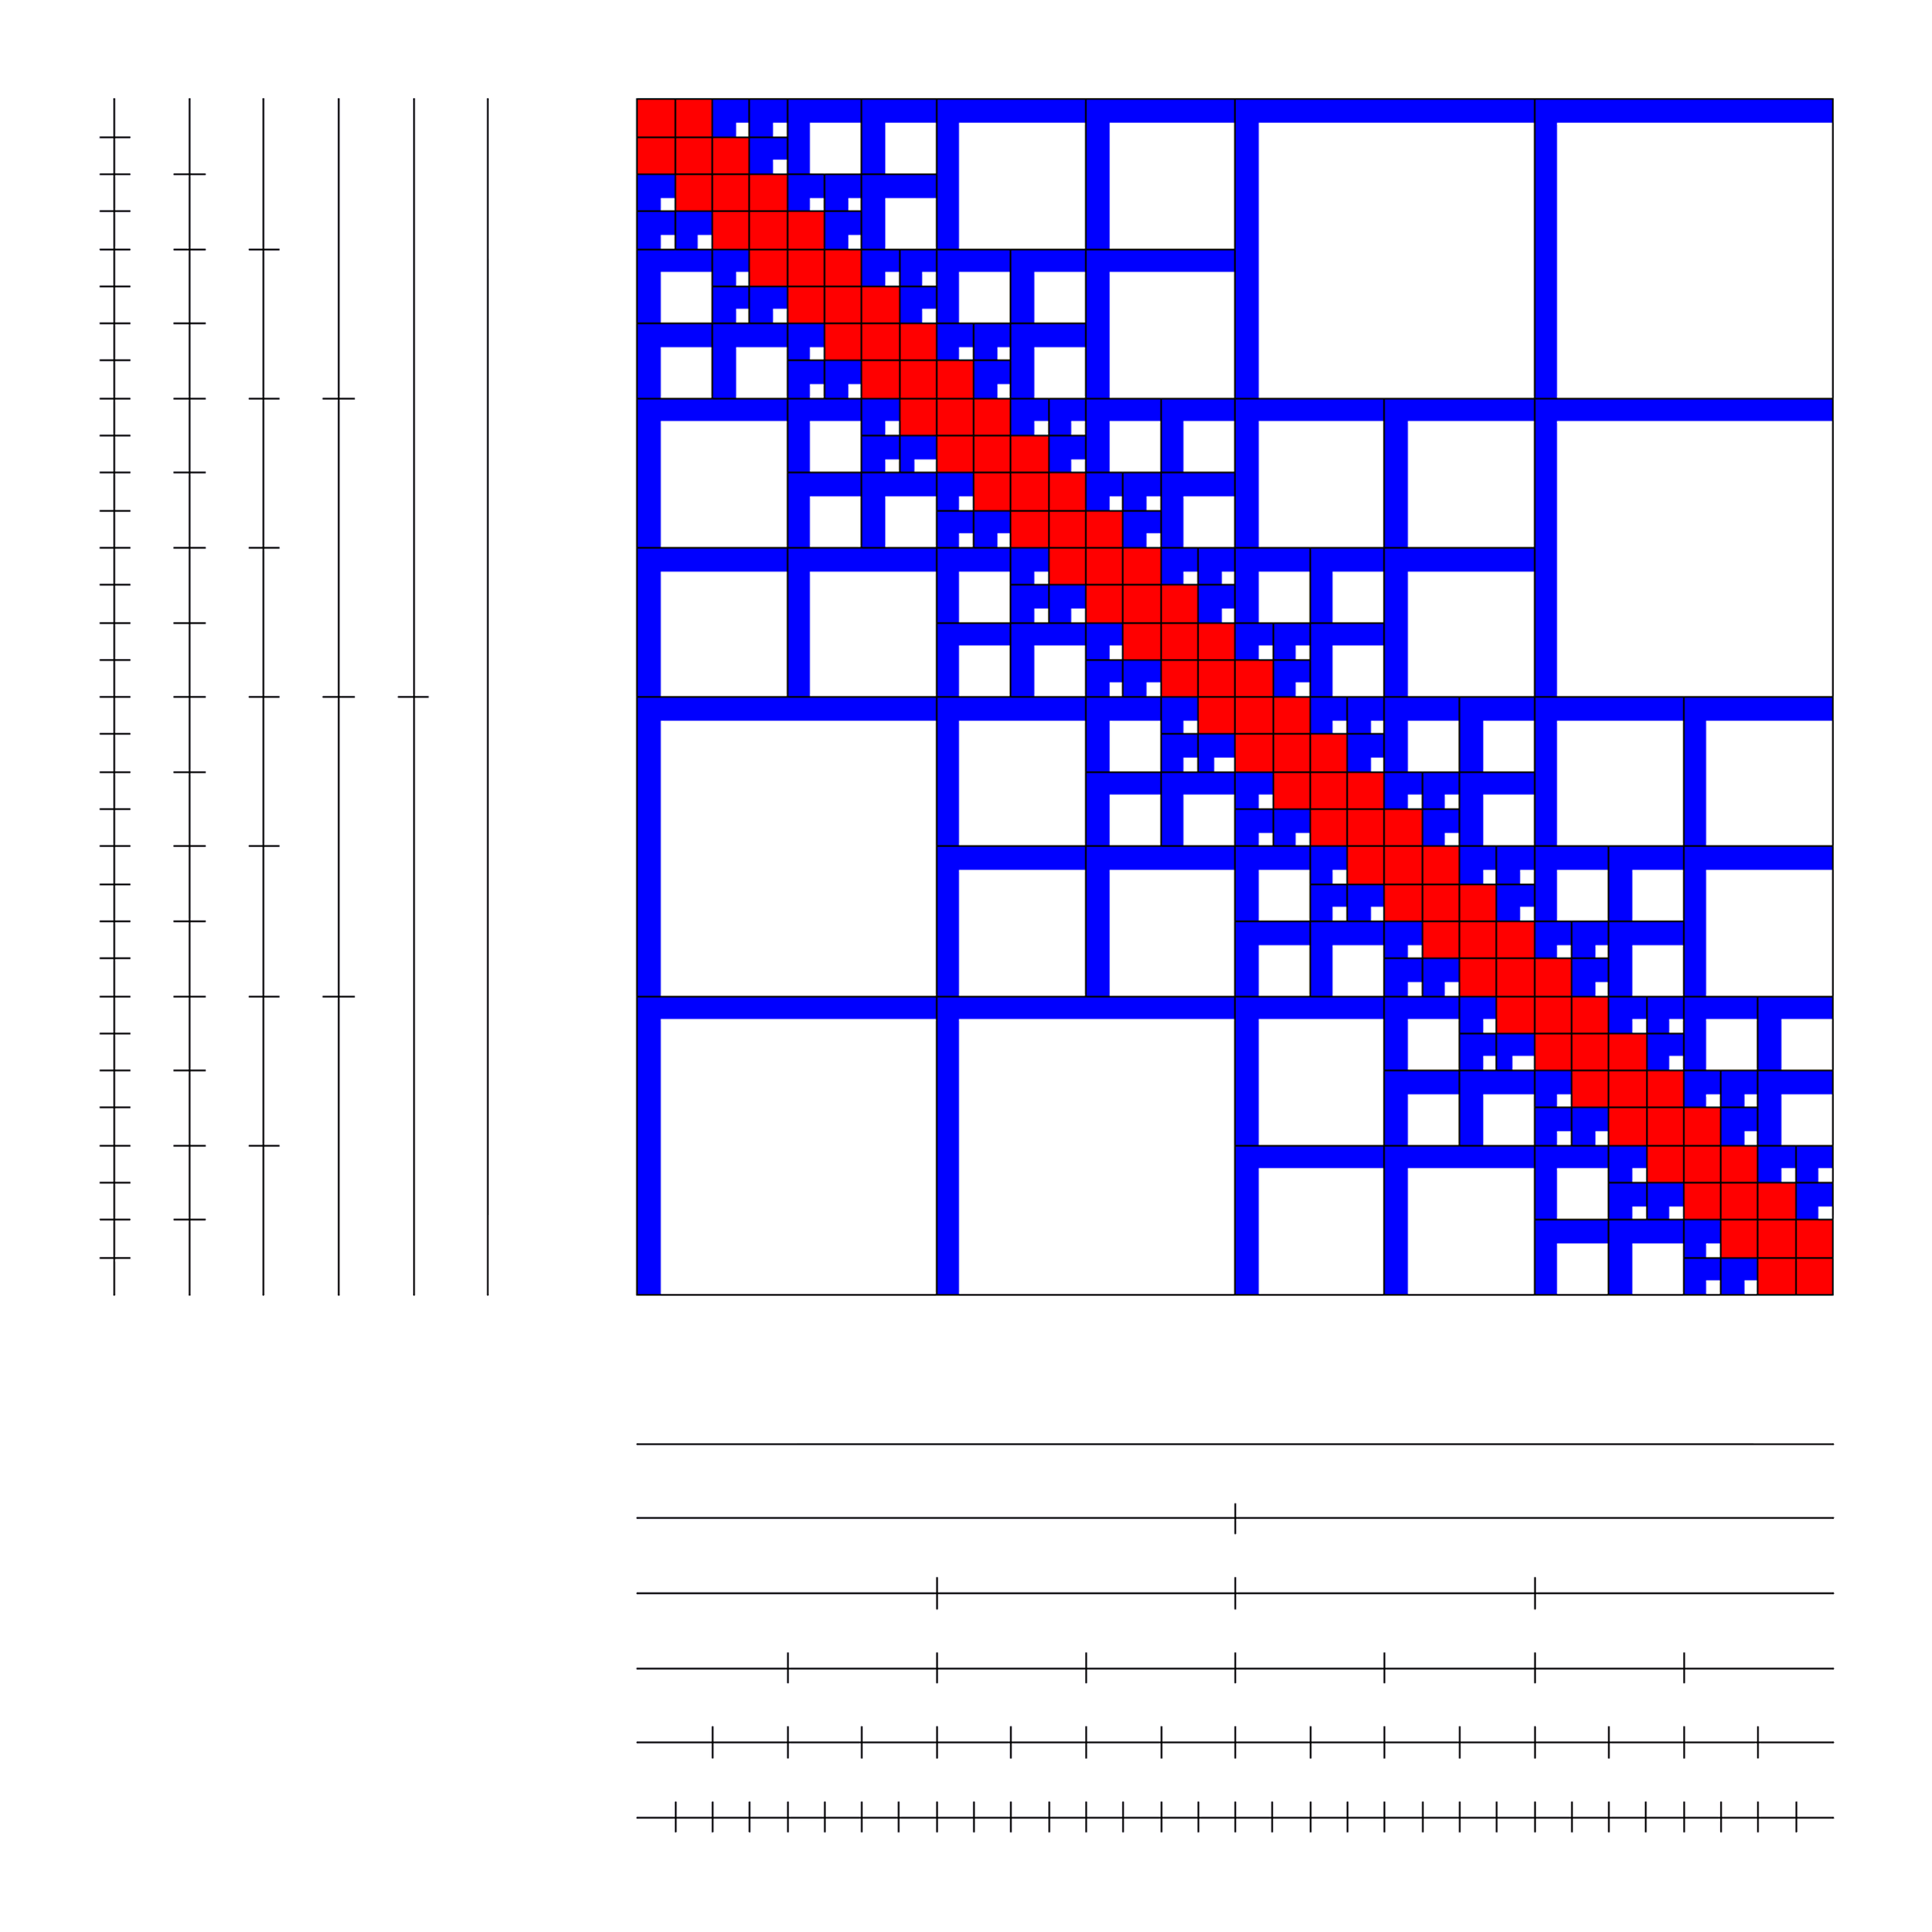
\includegraphics[width=0.7\textwidth]{img/h-matrix.png}
      \caption{Schematische Darstellung einer $\mathcal{H}$-Matrix. In blau sind die Matrizen $A_b$ und $B_b$, in rot die Matrizen $N_b$ gekennzeichnet. (Quelle: \citet{h2slides})}
      \label{fig:hmat}
    \end{figure}


    Für die Darstellung in Computern sind \hmat von besonderem Interesse, da sie sich durch die Zerlegung in \Rk-Matrizen besonders kompakt speichern lassen. Für eine $\mathcal{H}$-Matrix
    $M$ mit lokalem Rang $k$ existieren nach Definition Familien von Matrizen $\left(A_b\right)_{b \in \mathcal{L}^+\left(T_{X \times Y}\right)} \text{ und } \left(B_b\right)_{b \in \mathcal{L}^+\left(T_{X \times Y}\right)}$, mit 
    \begin{equation*}
      A_b \in \R^{t \times k}, B_b \in \R^{s \times k}, \left. M \right|_b = A_b\trans{B_b} \text{, für alle } b = t \times s \in \mathcal{L}^+\left(T_{X \times Y}\right).
    \end{equation*}
    So verbleiben nur noch für unzulässige Blöcke $b \in \mathcal{L}^-\left(T_{X \times Y}\right)$ vollbesetzte Matrizen $N_b = M|_b$, sogenannte \textit{Nahfeldmatrizen}.
    Das Tripel $\left( \left(A_b\right)_{b \in \mathcal{L}^+\left(T_{X \times Y}\right)} , \left(B_b\right)_{b \in \mathcal{L}^+\left(T_{X \times Y}\right)} , \left(N_b\right)_{b \in \mathcal{L}^-\left(T_{X \times Y}\right)} \right)$ bezeichnen wir als $\mathcal{H}$-
    Matrix-Darstellung der Matrix $M$. \citep{nichtlokop} 
    
    In \autoref{fig:hmat} ist eine $\mathcal{H}$-Matrix schematisch dargestellt. Für zulässige Blöcke sind die Matrizen $A_b$ und $B_b$ in blau 
    und die Nahfeldmatrizen $N_b$ in rot gekennzeichnet. Durch die Dicke der Matrizen $A_b$ und $B_b$ ist der lokale Rang $k$ dargestellt. die Speicherplatzersparnis ist dadurch gut zu erkennen.
    
    Gerade auch im Zusammenhang mit dieser Arbeit ist aber von noch größerem Interesse, dass auch Operationen wie Matrix-Vektor-Multiplikationen auf \Rk-Matrizen und damit auch auf \hmat wesentlich 
    effektiver implementiert werden können. \citet{h2diss} zeigt, dass die Matrix-Vektor-Multiplikation nur $k\left(n+m\right)$ statt $n \cdot m$ Operationen benötigt.
    
    \clearpage
    
    \subsection{Optimierung}
    \label{sec:optimierung}
    Im Folgenden wollen wir noch einige Überlegungen vorstellen, durch die \hmat noch speicherplatzsparender und noch effizienter in der Berechnung werden.
    
    \subsubsection{Zeilen- und Spaltenmatrizen}
    Bisher wurde eine hierarchische Matrix konstruiert, indem die Kernfunktion $g$ auf zulässigen Blöcken $b = \tau \times \sigma \in \mathcal{L}^+\left(T_{X \times Y}\right)$ durch die auf $\sigma$ 
    interpolierte Funktion
    \begin{equation*}
      g_\sigma\left(x, y\right) = \sum_{\nu \in \haken{k}} g\left(x, \xi_\inds{\nu}\right) \lag_\inds{\nu}\left(y\right)
    \end{equation*}
    approximiert wurde. Somit erhalten wir durch die punktweise Definition
    \begin{equation*}
      \left(A_b\right)_{x\nu} := g\left(x, \xi_\inds{\nu}\right) \text{ und } \left(B_b\right)_{y\nu} := \lag_\inds{\nu}\left(y\right) \text{ für alle } x \in \tau \text{ und } y \in \sigma
    \end{equation*}
    Matrizen $A_b \in \R^{m \times k}$ und $B_b \in \R^{n \times k}$. Damit können wir die Matrix $G$ auf Blöcken $b \in \mathcal{L}^+\left(T_{X \times Y}\right)$ in der Form 
    \begin{equation*}
      \left(G|_b\right)_{xy} = g\left(x,y\right) \approx g_\sigma\left(x,y\right) = \left(A_b \trans{B_b}\right)_{xy},
    \end{equation*}
    also durch \Rk-Matrizen darstellen und erhalten so eine Darstellung als hierarchische Matrix. \citep{nichtlokop}
    
    Ein Blick auf die Definition der Matrix $B_b$ verrät, dass diese nicht von $\tau$ sondern ausschließlich von $\sigma$ abhängt. Wir können sie also für konstantes $\sigma$ für alle Blöcke 
    $\tilde b = \tilde \tau \times \sigma \in T_{X \times Y}$ durch eine Matrix
    \begin{equation*}
      \left(W_\sigma\right)_{y\nu} := \lag_\inds{\nu}\left(y\right)
    \end{equation*} 
    ersetzen. Anstatt also für jeden Block $b$ wieder eine eigene Matrix aufstellen zu müssen, können sich Blöcke mit gleichem Quellgebiet $\sigma$ die Matrizen teilen. Insbesondere muss diese 
    Matrix $W_\sigma$ auch nur einmal berechnet werden, womit ein erheblicher Teil des Rechnungsaufwands bei der Konstruktion von \hmat eingespart werden kann. Zudem können wiederum Operationen
    wie die Matrix-Vektor-Multiplikation effektiver durchgeführt werden, da auch hier die Matrix $W_\sigma$ ausgeklammert werden kann, und so nur einmal in die Berechnung einfließt. \citep{nichtlokop}
    
    \begin{defn}
      (Zeilen-/Spaltenmatrizen)\\
      Wir nennen Matrizen $W_\sigma \in \R^{\sigma \times k}$ wie oben \textit{Spaltenmatrizen} einer hierarchischen Matrix $G$. Bei Interpolation in der ersten Komponente nennen wir sie 
      entsprechend \textit{Zeilenmatrizen}.
    \end{defn}
    
    \begin{figure}[t]
      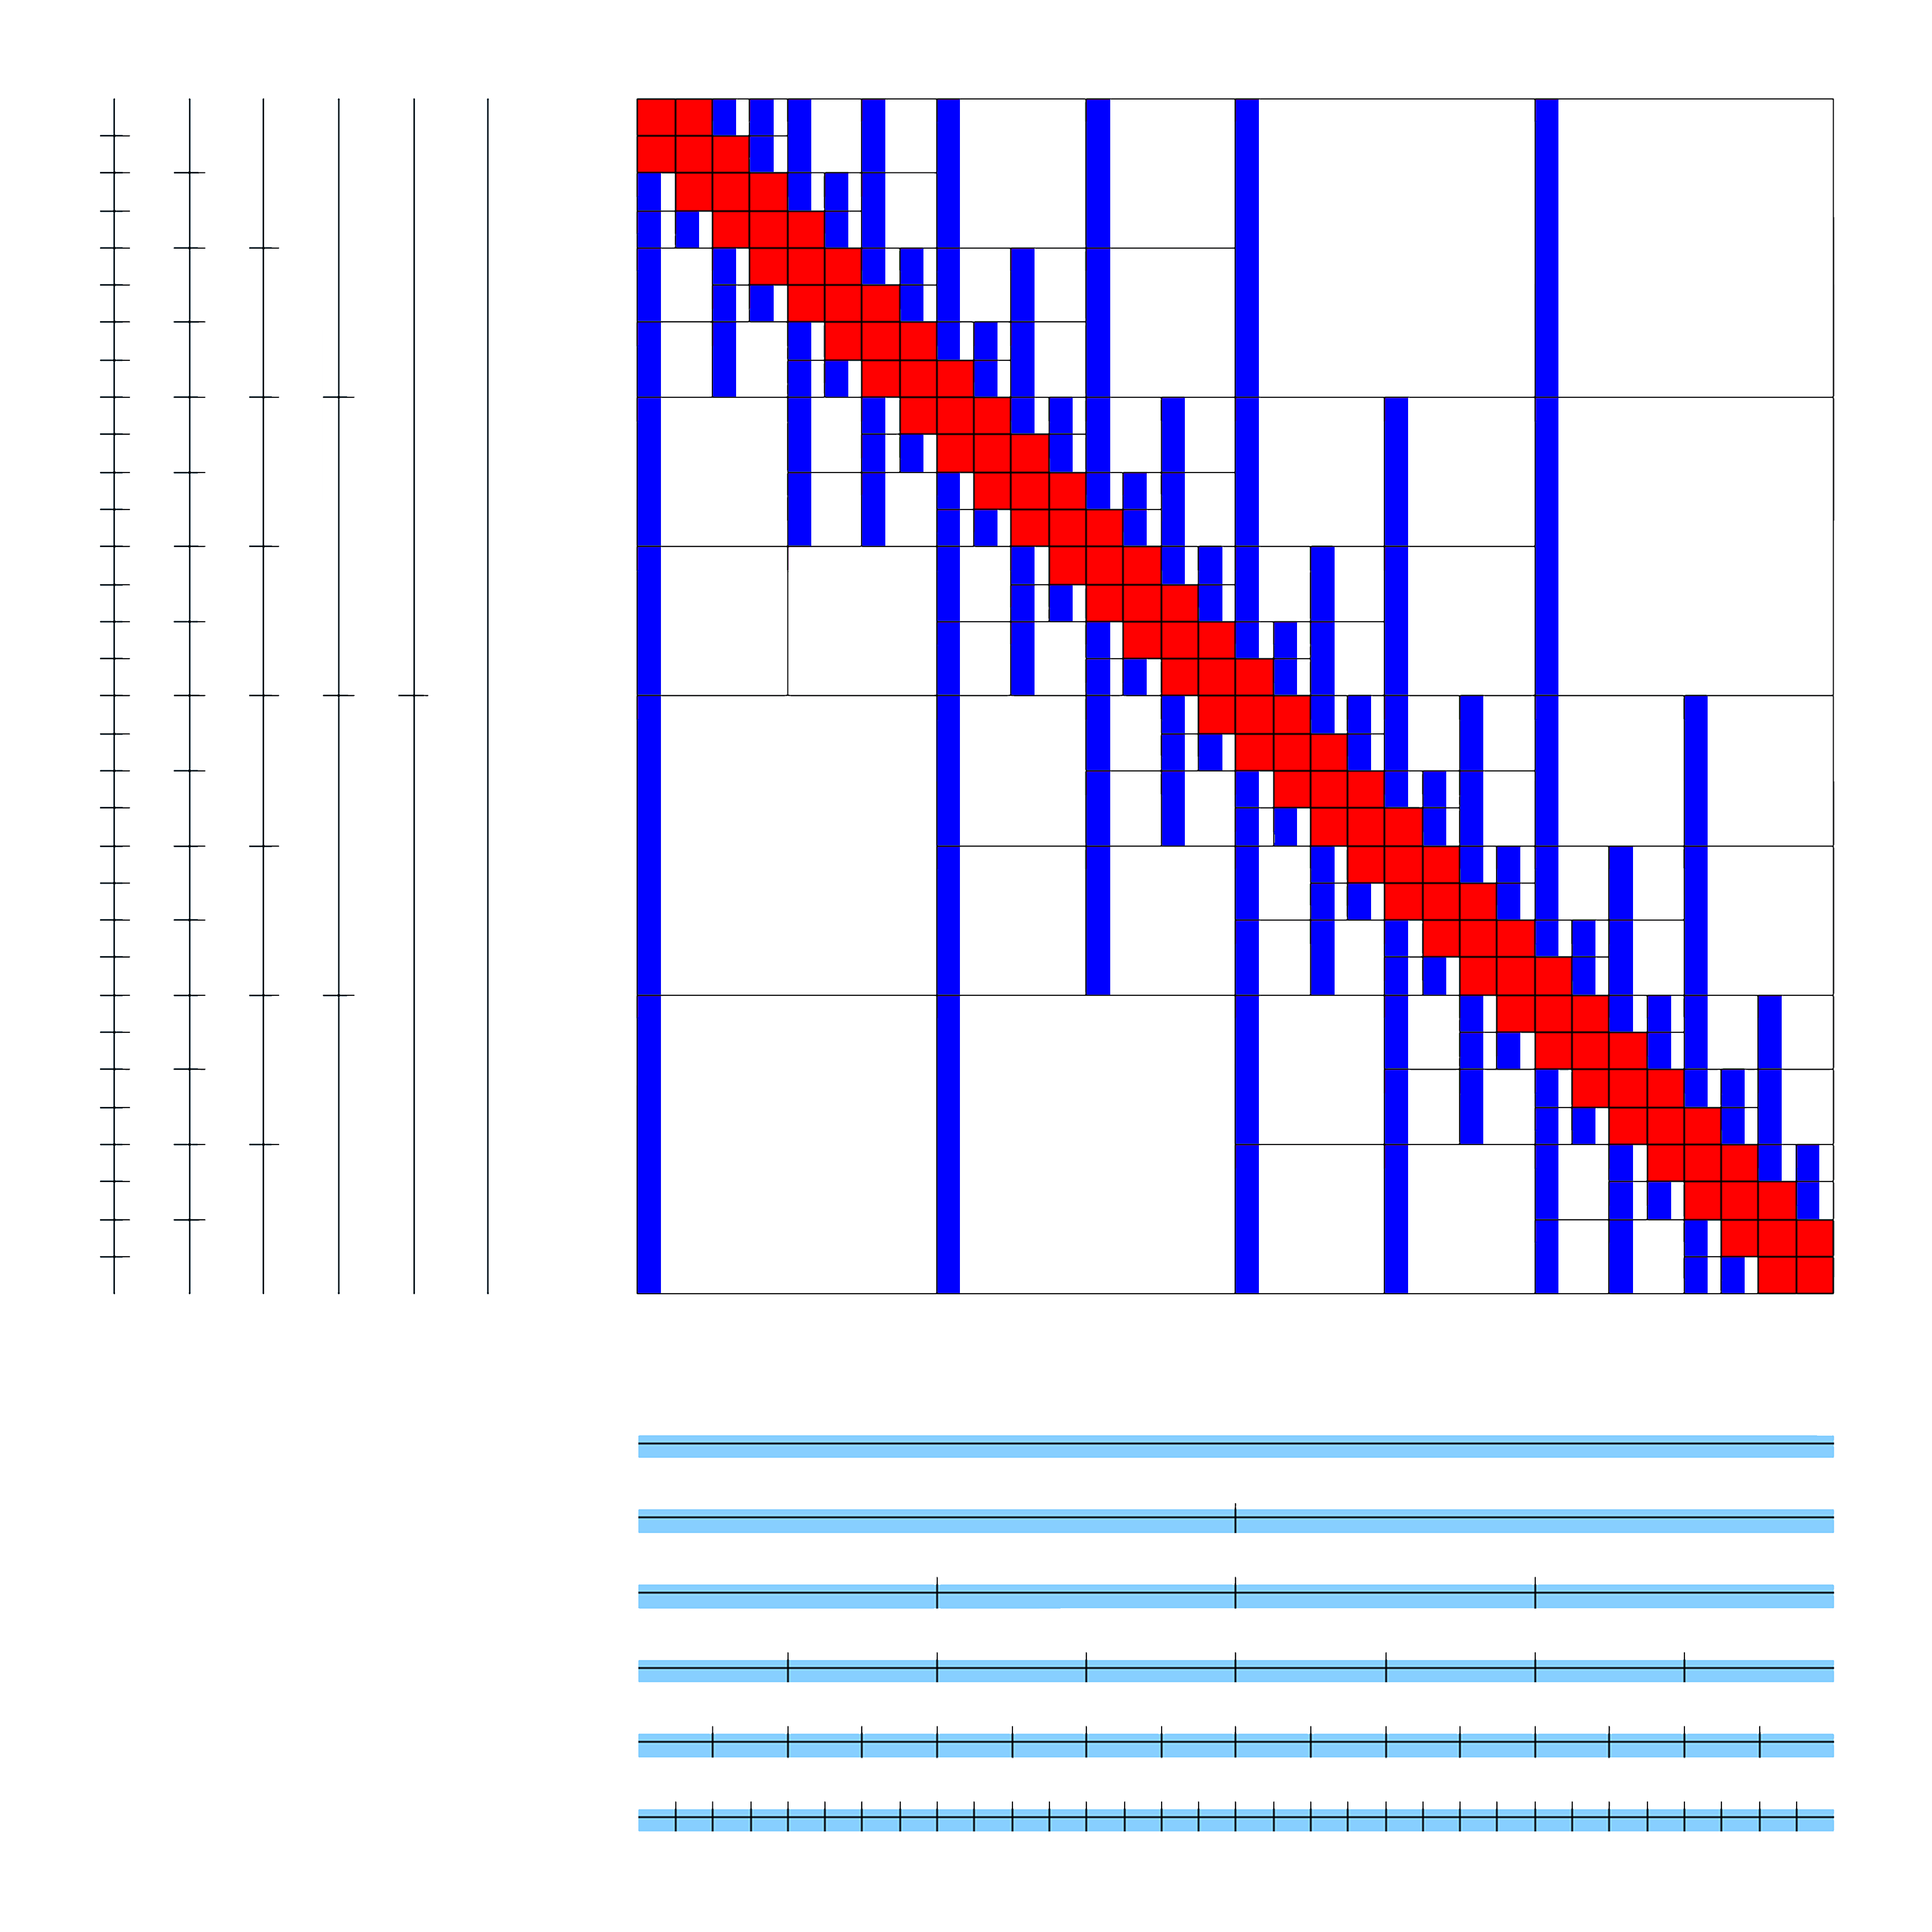
\includegraphics[width=0.7\textwidth]{img/semi-h2-matrix.png}
      \caption{Darstellung der Ersetzung der Matrizen $B_b$ durch Spaltenmatrizen $W_\sigma$. Letztere sind in hellblau auf dem Clusterbaum eingezeichnet. Die verbleibenden dunkelblauen 
	       Matrizen sind die Matrizen $A_b$. (Quelle: \citet{h2slides})}
      \label{fig:semi-h2}
    \end{figure}

    Dargestellt ist diese Optimierung in \autoref{fig:semi-h2}. In hellblau wurden die Spaltenmatrizen $W_\sigma$ auf dem Clusterbaum eingezeichnet. Die verbleibenden dunkelblauen Matrizen sind
    die nicht optimierten Matrizen $A_b$. Ein Vergleich der Häufigkeit der Matrizen $A_b$ und $W_\sigma$ verdeutlicht die zuvor beschriebene Ersparnis von Redundanz.

    
    \subsubsection{Transfermatrizen und Clusterbasis}
    \label{sec:transmat}
    Von \citet{h2approxint} wird auf folgende Eigenschaft der Interpolationsoperatoren hingewiesen:
    
%     Sei $\mathcal{T}_k$ der Polynomraum, der von Tensorprodukten \todo{genauer?} auf Polynomen von höchsten Rang $k$ aufgespannt wird. Dann ist der Interpolationsoperator eine \textit{Projektion}
%     auf diesen Raum. Wenn wir also für alle Cluster die Interpolationspolynome $\mathcal{T}_k$ verwenden, können wir die Lagrange-Polynome der Vatercluster verlustfrei aus den Lagrange-Polynomen
%     der zugehörigen Sohncluster konstruieren. 
\TODO{Polynomraum $\mathcal{T}_k$}
    
%     Es gilt wegen der Projektionseigenschaft für $\sigma \in T_X \backslash \mathcal{L}\left(T_X\right)$ und Söhne $\tilde \sigma \in sons\left(\sigma\right)$ für alle 
%     $\nu \in \haken{k}$:

    Alle Cluster wurden durch Polynome der selben Ordnung interpoliert. Wegen der Projektionseigenschaft des Interpolationsoperators folg damit für $\sigma \in T_X \backslash \mathcal{L}\left(T_X\right)$ 
    und Söhne $\tilde \sigma \in sons\left(\sigma\right)$ und für alle $\nu \in \haken{k}$:
    \begin{equation*}
      \lag_\inds{\nu} = \mathfrak{I}_{\tilde \sigma}[\lag_\inds{\nu}] = \sum_{\tilde \nu \in \haken{k}} \lag_\inds{\nu}\left(\xi_{\tilde \sigma,\tilde \nu}\right) \lag_{\tilde \sigma,\tilde \nu}.
    \end{equation*}
    
    Anstatt also auf jeder Ebene des Clusterbaumes eine vollständige Matrix $W_\sigma \in \R^{\sigma \times k}$ aufzustellen, genügt es für jeden Sohncluster $\tilde \sigma \in sons\left(\sigma\right)$
    Matrizen $E_{\tilde \sigma} \in \R^{k \times k}$ mit $\left(E_{\tilde \sigma}\right)_{\tilde\nu , \nu} := \lag_\inds{\nu}\left(\xi_{\tilde \sigma, \tilde \nu}\right)$ zu speichern. Dies führt zu folgender Definition:
    
    \begin{defn}
      (Transfermatrix, Clusterbasis)\\
      Sei $T_X$ ein Clusterbaum mit einer Familie von Spalten- (bzw. Zeilen-)matrizen $W = \left(W_\sigma\right)_{\sigma \in T_X}$. Existiert eine Familie $E = \left(E_\sigma\right)_{\sigma \in T_X}$ von 
      $\left(k \times k\right)$-Matrizen mit der
      Eigenschaft
      \begin{equation*}
	\left. V_\sigma \right|_{\tilde \sigma \times k} = V_{\tilde \sigma} E_{\tilde \sigma} \ \ \ \ \ \ \ \ \ \ \ \ \text{für alle } 
	\sigma \in T_X \backslash \mathcal{L}\left(T_X\right) \text{ und } \tilde \sigma \in sons\left(\sigma\right),
      \end{equation*}
      so nennen wir $V$ eine \textit{(geschachtelte) Clusterbasis} (von Rang $k$) für den Clusterbaum $T_X$. Die Matrizen der Familie $E$ heißen die korrespondierenden \textit{Tranfermatrizen}.
      \citep{nichtlokop}
    \end{defn}

    Mit der \textit{geschachtelten Darstellung} $\left(\left(W_\sigma\right)_{\sigma in \mathcal{L}\left(T_X\right)} , \left(E_\sigma\right)_{\sigma \in T_X \backslash \mathcal{L}\left(T_X\right)}\right)$ der Clusterbasen haben wir nun also eine 
    noch kompaktere Darstellung der Matrizen $B_b$.
    
    
    

    \subsubsection{Interpolation in beiden Komponenten}
    Auch in diesem Abschnitt folge ich dem Aufbau von \citet{nichtlokop}.
    
    Wir haben bereits einige Eigenschaften der Matrizen $B_b$ beziehungsweise $W_\sigma$ identifiziert, die sich zur Effektivitätssteigerung nutzen lassen.
    Leider bleiben die Speicherplatzineffizienz und der höhere Rechenaufwand für die Matrizen $A_b$ bestehen, die die positiven Eigenschaften der Matrizen $W_\sigma$ nicht teilen. Allerdings 
    haben wir die Matrizen $W_\sigma$ einfach punktweise aus den Lagrange-Polynomen bei der Interpolation definiert. Es liegt also nahe eine Interpolation nicht nur in einer, sondern in beiden 
    Variablen durchzuführen. Wir wählen also Interpolationspunkte $\xi_\indt{1}, \dots , \xi_\indt{k}$ und erhalten wiederum mit den zugehörigen Lagrange-Polynomen 
    $\lag_\indt{1}, \dots, \lag_\indt{k}$:
    \begin{equation*}
      g\left(x,y\right) \approx \tilde g\left(x,y\right) = \sum_{\mu \in \haken{k}} \sum_{\nu \in \haken{k}} \lag_\indt{\mu}\left(x\right) g\left(\xi_\indt{\mu}, \xi_\inds{\nu}\right) \lag_\inds{\nu}\left(y\right).
    \end{equation*}
    Mit 
    \begin{equation*}
      \left(S_b\right)_{\mu\nu} := g\left(\xi_\indt{\mu}, \xi_\inds{\nu}\right), \ \mu,\nu \in \haken{k}
    \end{equation*}
    erhalten wir eine Familie von Koeffizientenmatrizen $\left(S_b\right)_{b \in \mathcal{L}^+\left(T_{X \times Y}\right)} \in \R^{k \times k}$, die weder von $x$, noch von $y$ anhängt, sondern lediglich von den 
    Interpolationspunkten.
    Außerdem haben wir durch die neuerliche Interpolation die Abhängigkeit von $x$ wiederum auf Lagrange-Polynome beschränkt und erhalten so Matrizen $V_\tau \in \R^{\tau \times k}$ durch
    die Festlegung
    \begin{equation*}
      \left(V_\tau\right)_{x\mu} := \lag_\indt{\mu}\left(x\right).
    \end{equation*}
    Insgesamt erhalten wir also für alle $b = \tau \times \sigma \in \mathcal{L}^+\left(T_{X \times Y}\right)$
    \begin{equation*}
      \left. G \right|_b \approx \left. \tilde G \right|_b = V_\tau S_b \trans{W_\sigma}.
    \end{equation*}
    
    Die Matrizen $V_\tau$ haben dieselben Eigenschaften wie die Matrizen $W_\sigma$. Beide lassen sich also nicht nur effizient speichern, sondern auch effizient konstruieren. Außerdem 
    brauchen sie auf Grund der Entkoppelung von $\tau$ und $\sigma$ jeweils nur einmal aufgestellt zu werden. Da die Matrizen $S_b$, die die Kopplung zwischen den Clustern 
    $\tau$ und $\sigma$ beschreiben, wiederum verhältnismäßig klein sind, lassen sich diese wiederum auch effektiv verarbeiten.
    
    \subsection{\hquad}
    \label{sec:hquad}
      Die Überlegungen der letzten Abschnitte fließen nun in der Definition der \hquad zusammen.
      
      \begin{defn}
	(\hquad)\\
	Sei $T_{X \times Y}$ ein streng zulässiger Blockbaum, $k \in \N_0$ und seien $V$ und $W$ Clusterbasen des Ranges $k$ für die Clusterbäume $T_X$ und $T_Y$. Eine Matrix 
	$M \in \R^{X \times Y}$ heißt \textit{$\mathcal{H}^2$-Matrix} mit Zeilenbasis $V$ und Spaltenbasis $W$, falls für alle zulässigen Blattblöcke 
	$b = \tau \times \sigma \in \mathcal{L}^+\left(T_{X \times Y}\right)$ eine Matrix $S_b \in R^{k \times k}$ existiert, sodass
	\begin{equation*}
	  \left. M \right|_b = V_\tau S_b \trans{W_\sigma}
	\end{equation*}
	erfüllt ist. Die Familie $\left(S_b\right)_{b \in \mathcal{L}^+\left(T_{X \times Y}\right)}$ bezeichnen wir als Familie der \textit{Kopplungsmatrizen}.
      \end{defn}
      
      Für unzulässig Blattblöcke $b = \tau \times \sigma \in \mathcal{L}^-\left(T_{X \times Y}\right)$ verbleiben, wie auch bei den \hmat, die vollbesetzten Nahfeldmatrizen $N_b$.
      
      Mit geschachtelten Darstellungen 
      \[
      \left( 
	\left(V_\tau \right)_{\tau in \mathcal{L}\left(T_X\right)} , \left(E_\tau\right)_{\tau \in T_X \backslash \mathcal{L}\left(T_X\right)} \right) \text{ und }
	\left( \left(W_\sigma\right)_{\sigma in \mathcal{L}\left(T_Y\right)} , \left(F_\sigma\right)_{\sigma \in T_Y \backslash \mathcal{L}\left(T_Y\right)}
      \right) 
      \]
      der Clusterbasen $V$ und $W$ bezeichnen wir das Tupel
      \[
       \left(
	\left(S_b\right)_{b \in \mathcal{L}^+\left(T_{X \times Y}\right)} , \left(N_b\right)_{b \in \mathcal{L}^-\left(T_{X \times Y}\right)},
	\left(V_\tau\right)_{\tau in \mathcal{L}\left(T_X\right)} , \left(E_\tau\right)_{\tau \in T_X \backslash \mathcal{L}\left(T_X\right)},
	\left(W_\sigma\right)_{\sigma in \mathcal{L}\left(T_Y\right)} , \left(F_\sigma\right)_{\sigma \in T_Y \backslash \mathcal{L}\left(T_Y\right)}
       \right)
      \]
      als $\mathcal{H}^2$-Matrix-Darstellung der Matrix $M$.

      Von \citet{datasparse} wird eine vollständige Charakterisierung der \hquad vorgenommen. Dadurch wird ein für uns entscheidender Unterschied zwischen \hmat und \hquad deutlich:
      Bei \hmat müssen die zu den zulässigen Blöcken $b =\tau \times \sigma \in \mathcal{L}^+\left(T_{X \times Y}\right)$ gehörige Matrizen $\left. M\right|_{\tau \times \sigma}$ niedrigen Rang besitzen.
      Bei \hquad hingegen müssen die deutlich größeren Matrizen $\left. M\right|_{\tau \times R_\tau}$ und $\left. M\right|_{C_\sigma \times \sigma}$ für alle Cluster $\tau \in T_X$ und $\sigma\in T_Y$
      niedrigen Rang besitzen. Dabei sind für alle $\tau \in T_X$ und $\sigma \in T_Y$ definiert:
      \[
	R_\tau := \bigcup_{r \in row(\tau)} r , \ \ \ \ \ \ \ \ C_\sigma := \bigcup_{c \in col(\sigma)} c,
      \]
      \[
       row(\tau) := \{ s \in T_Y \ | \ \exists \tilde \tau \in T_X \colon \ \tilde \tau \times s \in \mathcal{L}^+\left(T_{X \times Y}\right) \wedge \tau \in sons^*(\tilde \tau) \},
      \]
      \[
       \ col(\sigma) := \{ t \in T_X \ | \ \exists \tilde \sigma \in T_Y \colon \ t \times \tilde \sigma \in \mathcal{L}^+\left(T_{X \times Y}\right) \wedge \sigma \in sons^*(\tilde \sigma) \}.
      \]
      Dieser Unterschied ist in \autoref{fig:hh2diff} bildlich dargestellt:
      
      \begin{figure}[b]
	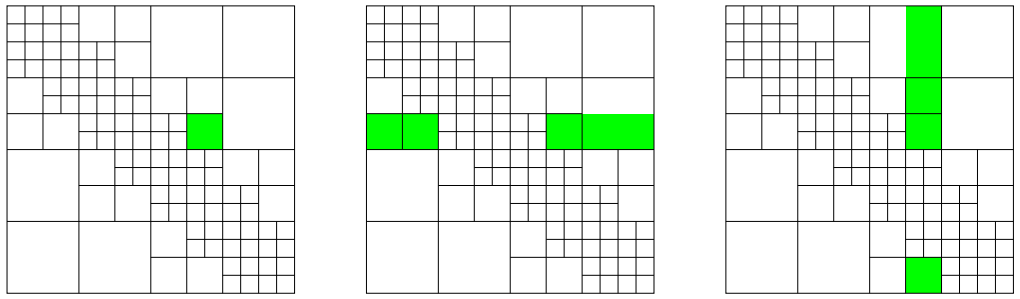
\includegraphics[width=\textwidth]{img/H_H2_diff.png}
	\caption{Vergleich zwischen $\mathcal{H}$- und $\mathcal{H}^2$-Matrix: Bei ersterer müssen nur einzelne Teilmatrizen niedrigen Rang besitzen, bei letzterer ganze Zeilen- und Spaltenblöcke.
	(Quelle: \citet{nichtlokop})}
	\label{fig:hh2diff}
      \end{figure}


      Mit den \hquad haben wir also eine sehr effiziente Teilmenge der hierarchischen Matrizen gefunden, die sich noch kompakter speichern lassen und mit denen Berechnungen noch effizienter 
      durchgeführt werden können.
  \clearpage
  
  \section{Paralleles Rechnen}
  \label{sec:parrech}
  Bereits in \autoref{sec:mot} wurde gezeigt, dass das Problem der gravitationellen Wechselwirkungen in unserer Galaxie mit einem aktuellen Computer nicht ohne 
    weiteres lösbar ist. 
    Konnten sich früher Programmierer darauf verlassen, dass in einigen Jahren eine deutlich schnellere Prozessorgeneration erscheinen würde, so dass Probleme ohne 
    weitere Änderungen schneller gelöst werden könnten, ist dies heute leider nicht mehr der Fall. 
    
    Grund hierfür ist die Physik. Dazu ein kleines Rechenexperiment: Nehmen wir einen Prozessorchip von etwa einem Zentimeter Durchmesser an und vergegenwärtigen wir 
    uns die Lichtgeschwindigkeit $c \approx 3\cdot10^{10}$ \footnote{Bureau International des Poids et Mesures [1975], \textit{Resolution 2 of the 15th CGPM},\\URL:
    https://www.bipm.org/en/CGPM/db/15/2/ Abgerufen am 16.07.2018}. Licht könnte diesen Chip also etwa 30 Milliarden mal pro Sekunde durchqueren, was 30 Gigahertz
    entspräche. Bedenkt man, dass man in Prozessoren mit Elektrizität arbeitet und somit beispielsweise mit kapazitären Effekten und proportional zur Taktfrequenz steigender
    Verlustleistung zu kämpfen hat, sind die 3 Gigahertz aktueller Mittelklasseprozessoren durchaus nicht zu verachten.
    
    Zwar wäre eine Möglichkeit die Chips weiter zu verkleinern, jedoch machen dem Fortschritt hier quantenmechanische Phänomene aktuell noch einen Strich durch die Rechnung.
    Ein gängiger und gangbarer Lösungsweg besteht in der Parallelisierung von Soft- und Hardware. Durch das gleichmäßige Verteilen eines Algorithmus auf mehrere Prozessoren
    kann die Gesamtlaufzeit entsprechend verringert werden. Unter optimalen Bedingungen könnte theoretisch eine Verdopplung der Prozessoranzahl eine Halbierung der Laufzeit
    bewirken. Heute haben daher die meisten Prozessoren nicht mehr nur einen Rechenkern, sondern mehrere und für die Berechnung großer mathematischer Probleme arbeiten oft viele
    Rechner zusammen an der Lösung. \citep{hpcskript}
    
    Ein weiterer Grund für parallele beziehungsweise verteilte Rechnersysteme ist die Diskrepanz zwischen vorhandenem und benötigtem Speicher. Beispielsweise hat der diesbezüglich größte
    Computer im Rechenzentrum der Christian-Albrecht-Universität Kiel einen Hauptspeicher von 768 GB. Ein aktuelles, speicherintensives Problem ist ein engmaschiges 
    Klimamodell der Erde. Bei einer Dichte von einer Masche alle 1,56 km in Äquatornähe wird der Gesamtspeicherbedarf auf etwa 24000 GB geschätzt \citep{climate}. Ein Problem
    dieser Größe passt nicht mehr in den Hauptspeicher eines Computers.
    Hinzu kommt die Skalierbarkeit solcher Probleme: Angenommen ein Hauptspeicher von 24000 GB stünde auf einem Computer zur Verfügung. Warum bei einer Maschendichte von 
    1,56 km stehen bleiben und nicht noch feiner auflösen um noch genauere Berechnungen durchzuführen?
    Warum bei der Berechnung der gravitationellen Wechselwirkungen bei den Sonnen unserer Galaxie stehen bleiben und nicht die Planeten, Monde oder noch kleinere Himmelskörper mit einbeziehen? 
    Diese Probleme, und damit auch der Speicherbedarf, lassen sich also nahezu beliebig vergrößern. Wir benötigen also eine Möglichkeit, günstig genügend Hauptspeicher zur Verfügung zu stellen.
    Das Vernetzen von Computern und das Verteilen der Arbeit und der Daten durch parallel arbeitende Algorithmen auf die vernetzten Rechner ist ein Lösungsansatz für dieses Problem.
    
    Im folgenden Kapitel wird kurz skizziert, wie parallel arbeitende Hardware gestaltet sein kann und welche Vor- und Nachteile und welche Herausforderungen damit einhergehen. Grundbegriffe
    der Computerarchitektur werden vorausgesetzt, da eine Einführung den Umfang dieser Arbeit sprengen würde.
    
    \subsection{Parallele Hardware}
    \label{sec:parhard}
      \subsubsection{Prozessor}
      \label{sec:processor}
      \citet{flynn} klassifiziert vier unterschiedliche Architekturen von Rechnern. Dabei unterteilt er nach der Möglichkeit des Prozessors, zu einem Zeitpunkt einzelne oder mehrere
      Instruktionen beziehungsweise Datensätze zu verarbeiten (vgl. \autoref{tab:flynn}).
      \begin{table}[tb]
	\centering
	\begin{tabular}{|p{3.5cm}|p{4cm}|p{4cm}|}
	  \hline
			                             & eine Instruktion \newline (single instruction)       & mehrere Instruktionen \newline (multiple instruction) \\
	  \hline
	  ein Datensatz \newline (single data)       & SISD: konventioneller \newline einkerniger Prozessor & MISD: Spezialrechner                                  \\
	  \hline
	  mehrere Datensätze \newline (multiple data)& SIMD: Vektorrechner                                  & MIMD: Multicore; \newline Clustersystem               \\
	  \hline
	\end{tabular}
	\caption{Flynnsche Klassifikation mit Beispielen.}
	\label{tab:flynn}
      \end{table}
      
      Vor einigen Jahrzehnten waren die meisten Prozessoren in PCs noch SISD-Architekturen. Sie hatten einen Prozessor mit einem einzelnen Kern; konnten also zu jedem Zeitpunkt nur eine Instruktion
      auf einem Datensatz ausführen. Heute sind Multicore-Prozessoren üblich. Auf einem Prozessorchip finden sich hierbei mehrere Rechenkerne. Die einzelnen Kerne sind unabhängig voneinander; sie 
      verwalten eigene Register und führen eigene Instruktionen aus. Daher zählen Multicore-Prozessoren zu den MIMD-Architekturen. Zu diesen Architekturen gehören ebenfalls die später erläuterten 
      \hyperref[sec:netzwerk]{Clustersysteme}. \citep{flynn, multicore}
      
      MIMD-Architekturen sind auf Grund ihrer autonom arbeitenden und programmierbaren Prozessoren sehr flexibel und können viele Probleme effizient lösen. Die Autonomie der Prozessoren
      stellt die Programmierung aber auch vor Herausforderungen. Durch die asynchrone Ausführung der Programme wird das Verhalten des gesamten Systems schwer vorhersagbar. \citep{hpcskript}
      
      MISD-Architekturen, also solche, in denen parallel auf einem Datum mehrere Instruktionen ausgeführt werden können, sind nur in Spezialrechnern zu finden und für die Lösung der meisten
      Probleme nicht geeignet. \citep{architect, korbler}
      
      SIMD-Architekturen hingegen, in denen auf mehreren Daten parallel die gleiche Instruktion ausgeführt werden kann, sind durchaus gängig.
      Ihr Hintergrund sind Algorithmen, die auf ganzen Reihen von Daten immer wieder dieselbe Operation ausführen. Während beim Ansatz der MIMD-Architekturen die Operationen dynamisch auf die
      einzelnen Recheneinheiten verteilt werden, ist der Ansatz von SIMD-Architekturen beziehungsweise von Vektorrechnern, die Anzahl der Rechenwerke in den Recheneinheiten zu erhöhen 
      und eine Operation für mehrere Daten gleichzeitig auszuführen. Zum Beispiel werden für die Berechnung der Gravitationskräfte für viele Körper immer wieder dieselben Operationen 
      verarbeitet. Anstatt diese also für jedes einzelne Paar von Körpern durchzuführen, könnten sie für mehrere Paare von Körpern gleichzeitig durchgeführt werden.
      
      Der Name ``Vektorrechner'' leitet sich von der Anlehnung an die kartesische Geometrie her, in der ein Vektor ein Tupel von Zahlen ist. Entsprechend werden Daten desselben Typs ebenfalls 
      als Vektoren bezeichnet. Um solche Vektoren handhaben zu können, verfügen Vektorrechner über spezielle Vektorregister, die mehrere Daten gleichzeitig fassen können. Für jedes einzelne
      Datum innerhalb dieser Register ist dann jeweils ein eigenes Rechenwerk im Kern zuständig. \citep{hpcskript}
      
      Prozessoren laden in der Regel nicht nur ein einzelnes Datum, sondern gleich eine sogenannte \textit{cache line} aus dem Hauptspeicher. Daher ist es sinnvoll, 
      um SIMD-Parallelisierung optimal ausnutzen zu können, die Daten im Hauptspeicher anhand dieser cache lines anzuordnen. Dazu müssen in der Regel explizite Methoden zum Anfordern von 
      \wlabel{\textit{aligned memory}}{w:aligned} verwendet werden. Außerdem müssen die parallel zu verarbeitenden Daten im Hauptspeicher direkt hintereinander und nicht durch andere Daten 
      unterbrochen auftauchen. Nehmen wir an, wir wollten die Daten der Körper, die für die Berechnung der Gravitationskräfte benötigt werden, in einer Struktur zusammenfassen. Wollen wir
      Daten zu vielen dieser Körper speichern, so wäre es in Bezug auf Vektorrechner nicht sinnvoll, ein Array dieser Strukturen anzulegen (engl.: \wlabel{\textit{array of structs}}{w:aos}).
      Dabei würden die im Sinne der Vektorisierung zusammengehörigen Daten durch andere getrennt. Um eine Vektorisierung zu ermöglichen, ist es daher sinnvoll die Struktur so zu definieren,
      dass sie Arrays der benötigten Daten beinhaltet (engl.: \wlabel{\textit{struct of arrays}}{w:soa}). So kann sichergestellt werden, dass diese Daten im Hauptspeicher hintereinander stehen.
      \citep{hpcskript, architect}
      
      Viele aktuelle Multicore-Prozessoren verfügen zusätzlich über einige Möglichkeiten der Vektorisierung. Es existieren aber auch auf diese Art der Parallelisierung spezialisierte Prozessoren.
      \citep{architect}
      
      \subsubsection{Speicherverwaltung}
      \label{sec:speicher}
	In \autoref{sec:parrech} wurde bereits kurz erwähnt, dass bei Multicore-Prozessoren jeder Kern seine eigenen Register hat. Genau genommen verfügen die Kerne meist auch über privaten L1-,
	seltener über L2- oder L3-Cache. Diese sind meist \textit{shared} (dt.: gemeinsam genutzt). Shared Memory wird von allen Prozessoren gemeinsam verwaltet.
	
	Grundsätzlich können die heute üblichen MIMD Architekturen weiter anhand ihrer Speicherverwaltung unterteilt werden. Beim Shared-Memory-Modell wird ein globaler
	Speicher gemeinsam genutzt. Sie teilen sich also einen gemeinsamen Adressraum. Dies trifft in der Regel auf den Hauptspeicher, aber eventuell auch auf ebenen des Caches zu.
	Anders ist dies beim Distributed-Memory-Modell. Hier besitzt jeder Prozessor seinen eigenen Speicher. Distributed-Memory-Systeme sind in der Regel vernetzte Rechnersysteme. Allerdings wird
	auch auf Shared-Memory-Systemen durch moderne Betriebssysteme ein Distributed-Memory-Modell simuliert. Durch die Virtualisierung des Hauptspeichers etwa wird jedes Programm behandelt,
	als hätte es den Hauptspeicher für sich alleine. Dabei wird jedem Programm ein privater Bereich des Hauptspeichers zugewiesen. Das Programm nutzt diesen Bereich, als sei es der gesamte
	Hauptspeicher. \citep{korbler}
	
	Der Vorteil von gemeinsam genutztem Speicher ist, vorausgesetzt das Programm wurde entsprechend entworfen, dass die Ergebnisse eines Kerns den anderen automatisch auch zur Verfügung stehen. 
	Arbeiten  also mehrere Recheneinheiten gemeinsam an einem Problem, müssen die Ergebnisse einer Einheit den anderen also gegebenenfalls nicht explizit mitgeteilt werden. Dies vermeidet Overhead
	durch das Austauschen und Kopieren von Daten.
	Jedoch ist es bei privatem Cache möglich, diesen in größerer Nähe zum zugehörigen Kern auf dem Chip zu platzieren. Dies führt zu besseren Zugriffszeiten als gänzlich gemeinsam genutzter 
	Cache und wird daher auch oft verwendet. 
	
	Ein Nachteil von Shared-Memory-Systemen ist, dass der Schaltungsaufwand für den Zugriff auf den gemeinsam genutzten Speicher mit wachsender Anzahl Recheneinheiten rapide ansteigt
	\citep{hpcskript}. Außerdem können Race Conditions auftreten, die durch den gemeinsam genutzten Speicher verursacht werden. Diese können dazu führen, dass die Ergebnisse von Programmen
	unvorhersagbar werden.
	
	Beim Schreiben von parallelen Programmen ist also besondere Vorsicht geboten. Gegebenenfalls müssen Zugriffe auf gemeinsam genutzte Ressourcen zeitweise unterbunden werden, um Race Conditions
	zu vermeiden. Außerdem muss klar sein, welche Daten sich wo befinden, und ob sie gemeinsam genutzt werden oder nicht. Dies ist gegebenenfalls eine noch größere Herausforderung, wenn der Hauptspeicher 
	innerhalb eines parallelen Programms teilweise gemeinsam genutzt wird und teilweise verteilt ist.
	
      \subsubsection{Netzwerk}
      \label{sec:netzwerk}
		
	Wie bereits erwähnt gibt es Probleme, die für einen einzelnen Computer zu viel Hauptspeicher benötigen oder zu viel Rechenaufwand bedeuten. Daher ist es naheliegend, Computer zu Netzwerken,
	sogenannten \textit{Clustersystemen}, zusammenzuschließen. Hierbei können die vernetzten Computer, die als \textit{Knoten} des Clustersystems bezeichnet werden, über die 
	Netzwerkverbindung kommunizieren. Clustersysteme gehören zur Klasse der MIMD-Architekturen und stellen meist eine Mischform aus Distributed- und Shared-Memory-Modell dar: Jeder Knoten hat 
	seinen eigenen Hauptspeicher, der nicht mit den anderen Knoten geteilt wird; die einzelnen Knoten sind in der Regel aber Shared-Memory-Systeme. Meist verfügen die einzelnen Knoten über
	einen oder mehrere Multicore-Prozessor(en). \citep{cluster}
	
    \subsection{Parallele Software}
      Im vorherigen Abschnitt wurde die Entwicklung von einzelnen Computern mit einer Recheneinheit hin zu Clustersystemen skizzert, deren Knoten mit multiplen Recheneinheiten bestückt sind.
      
      Solange es sich um einen Computer mit Multicore-Prozessor handelt, ist bis dato keine Änderung an der Software notwendig, um auf diesem Multicore-Prozessor lauffähig zu sein. 
      Auf einem Computer läuft in der Regel nicht nur ein einzelnes Programm, sondern mindestens noch ein Betriebssystem und meist auch noch einige weitere Programme.
      Der Prozessor kann nun lediglich mehrere Programme echt parallel verarbeiten.
      
      Allerdings profitiert ein Programm bis dato noch wenig von parallel arbeitender Technologie; es wird nur gegebenenfalls seltener von anderen Programmen unterbrochen.
      Soll sich das Potential der Parallelität für ein Programm voll entfalten, so muss das Programm selbst parallel arbeiten, um so mehrere Kerne beziehungsweise mehrere Knoten eines 
      Clusters nutzen zu können. 
      
      Dazu sind natürlich auch entsprechende Entwicklungen im Bereich der Software notwendig. Zum einen muss es überhaupt möglich sein, mehrere Instanzen eines 
      Prozesses zu starten und diese zusammenarbeiten zu lassen. Dies impliziert aber wiederum die Schaffung von Möglichkeiten, die oben erwähnten Race Conditions zu vermeiden. Schließlich 
      müssen für Programme, die auf Clustersystemen arbeiten, Möglichkeiten geschaffen werden zu kommunizieren. Durch diese Kommunikation wäre es dann auch nicht mehr notwendig, alle Daten
      lokal abrufbar zu haben. Stattdessen wäre es möglich, die Datenmenge auf die Knoten zu verteilen und bei Bedarf zwischen Knoten auszutauschen. Erst dadurch sind Probleme wie die 
      Berechnung der Gravitationskräfte oder engmaschige Klimamodelle zu bewältigen.
      All diese Konzepte vorzustellen wäre im Rahmen dieser Arbeit nicht zielführend. Wir beschränken uns also auf die Einführung eines Konzeptes.
      
      \subsubsection{Das Message-Passing-Modell}
      \label{sec:mpm}
%       \begin{figure}[bt]%
% 	\centering%
% 	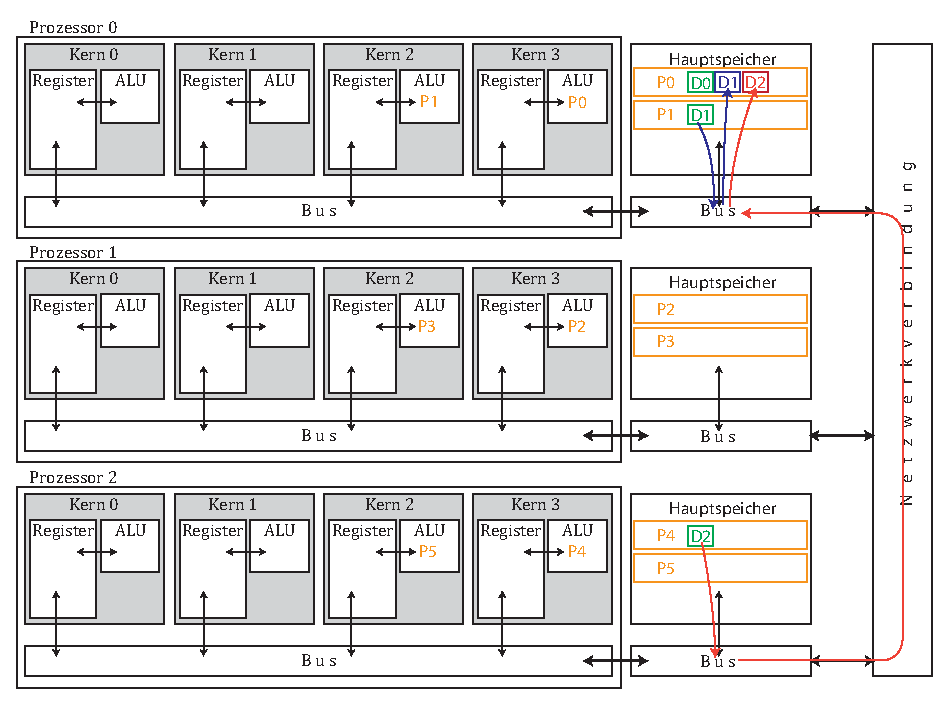
\includegraphics[width=0.9\textwidth]{img/multicorecluster_com.eps}%
% 	\caption{Eine Veranschaulichung des Message-Passings auf einem Clustersystem. In rot die Kommunikation zwischen zwei Knoten eines Clustersystems, in blau die Kommunikation innerhalb
% 	eines Knotens.}%
% 	\label{fig:message-passing}%
%       \end{figure}%
      Für unser Beispielproblem der Berechnung der Gravitationskräfte ist ein Programm vonnöten, das auf einem Clustersystem läuft und dessen Speicher verteilt verwaltet wird.
      Daher wird im folgenden Kapitel ein Parallel-Programing-Modell vorgestellt, das die Schwierigkeiten von Shared-Memory-Systemen umgeht und ein Konzept der Speicherverwaltung 
      und Kommunikation auf verteilten Rechnersystemen liefert.
      Dieses Konzept ist das sogenannte \textit{Message-Passing-Modell}. 
      Dieses Modell geht von einer Menge von \textit{autonomen} Prozessen aus, die
      \begin{enumerate}
       \item eindeutig benannt sind und
       \item jeweils über \textit{privaten Speicher} verfügen.
      \end{enumerate}
      Dies spezifiziert nicht, um welche Art Rechner(system) es sich handelt. Bei gemeinsam genutztem Hauptspeicher wird davon ausgegangen, dass jeder Prozess einen eigenen privaten 
      Bereich zugewiesen bekommt.
      
      Um nun Daten von einem Prozess $P_i$ an einen Prozess $P_j$ zu senden, muss $P_i$ explizit im Programmlauf seine Daten in Form einer Nachricht (engl.: message) verschiocken, und
      respektive $P_j$ diese Nachricht und damit die Daten in Empfang nehmen. 
%       \autoref{fig:message-passing} veranschaulicht die Wege der Nachrichten. Dabei bezeichnen $P_0,\dots,P_n$ die Prozesse und $D_0,\dots,D_2$ zugehörige Daten im Hauptspeicher. 
      
      Ein Nachteil des Message-Passing-Modells besteht in der Grundannahme von nicht gemeinsam genutztem Speicher.
      Jeder Prozess hat seine eigenen Kopien der benötigten Daten und Ergebnisse müssen explizit durch Nachrichten mitgeteilt und in die Speicherbereiche der anderen Prozesse kopiert werden. Dies
      macht das Programm aber auch weniger anfällig für Race-Conditions. Weitere Vorteile des Message-Passing-Modells sind:
      \begin{labeling}{Universalität }
	\item[Portabilität] Message-Passing ist spätestens seit \nameref{sec:mpi} (vgl.: \autoref{sec:mpi}) auf den meisten parallelen Plattformen einheitlich implementiert.
	\item[Universalität] Das Message-Passing-Modell stellt nur minimale Anforderungen an die zugrundeliegende Hardware. Es funktioniert einheitlich für vernetzte Systeme mit verteiltem 
			     Speicher ebenso wie für Shared-Memory-Systeme oder Kombinationen aus diesen.
	\item[Einfachheit] Das Modell unterstützt explizite Kontrolle über Referenzen zu Speicherzellen und erleichtert so auch Debugging.
      \end{labeling}
      Diese Vorteile machen das Message-Passing-Modell zu einem der Standardmodelle im High-Performance-Computing. \citep{ibm_mpm, anl_mpm, fsu_mpm}
    
  \clearpage
  
  \section{MPI}
  \label{sec:mpi}
      MPI (\textit{Message-Passing Interface}) ist eine Spezifikation für den Nachrichtenaustausch eines verteilten Systems. MPI richtet sich hauptsächlich nach dem 
    \textit{Message-Passing-Modell} (siehe \autoref{sec:mpm}).
    Erweitert wird das ``klassische'' Message-Passing-Modell unter anderem durch kollektive Kommunikationsmöglichkeiten, Remote-Speicherzugriff und parallele I/O-Operationen.
    Als Interface bietet MPI selbst keine Implementierung des Standards, sondern beschreibt Methoden und ihre Semantik.
    
    Das Ziel von MPI ist es, einen Standard für Programme zu liefern, die sich des Message-Passing-Modells bedienen, und somit zu Effizienz, Portabilität und Flexibilität
    beizutragen. \citep{mpiv31}
    
    \subsection{Geschichte}
      Bereits vor 1992 gab es Bibliotheken für paralleles Rechnen. Jedoch gab es keinen einheitlichen Standard und die meisten Bibliotheken waren systemspezifisch,
      sodass das Portieren von Programmen auf ein anderes System zumindest eine aufwendige Aufgabe war. Auch die Ansätze der Bibliotheken unterschieden sich teilweise
      stark. Ein weit verbreiteter Ansatz war allerdings auch damals schon das Message-Passing-Model. \citep{mpitut}
      
      Am 29. und 30. April 1992 begann mit dem \textit{Workshop on Standards for Message-Passing in a Distributed Memory Environment} am \textit{Center for Research on Parallel 
      Computing} in Williamsburg (Virginia) ein Prozess zur Standardisierung des Message-Passing-Ansatzes \citep{workshop}. Hier wurden die essentiellen Bestandteile eines 
      standardisierten Message-Passing-Interfaces diskutiert. An diesem Prozess waren rund 60 Personen von 40 verschiedenen Organisationen beteiligt, darunter die bedeutendsten
      Anbieter von Parallelrechnern sowie Forscher aus Universitäten, staatlichen Laboren und der Industrie. Die Ergebnisse wurden zunächst in einem vorläufigen Entwurf im
      November 1992 und schließlich in revidierter Fassung in einem Proposal, bekannt als MPI-1, veröffentlicht. \citep{mpi1}
      
      Eine Hauptabsicht von MPI-1 war es, erst einmal den ``Ball in's Rollen zu bringen'' und eine Diskussion anzuregen. Daher beschäftigte es sich noch hauptsächlich mit Point-to-Point-Kommunikation.
      Aktuell liegt MPI in der Version 3.1 vor und bietet neben der Point-to-Point-Kommunikation auch kollektive Routinen, nicht-blockierende Methoden, automatische Puffer-Verwaltung und vieles mehr.
      \citep{mpiv31}
      
      Das Interfaces wurden bald in den Programmiersprachen C und Fortran implementiert. Heute gibt es eine Vielzahl von Implementierungen; sowohl kostenfreie, wie  
      MPICH\footnote{Entwickler: Argonne National Laboratory -- Früheste Implementierung -- Bis heute weiterentwickelt -- URL: https://www.mpich.org/} oder
      Open MPI\footnote{Entwickler: Diverse -- Kombiniert Ansätze von FT-MPI, LA-MPI und LAM/MPI -- URL:https://www.open-mpi.org/},
      aber auch kostenpflichtige, wie die Implementierungen von Intel\footnote{https://software.intel.com/en-us/intel-mpi-library} oder IBM\footnote{https://www.ibm.com/de-de/marketplace/spectrum-mpi}. 
      
    \subsection{Point-to-Point-Kommunikation}
    \label{sec:ptpkom}
    Die Point-to-Point-Kommunikation ist das durch das Message-Passing-Modell beschriebene Herzstück von MPI.  
    Die Standardmethoden in C-Syntax sind:
    \begin{lstlisting}[language=C, label=lst:p2p_standard, caption={Die Syntax der standard Sende- und Empfangsoperationen}, numbers=none]
	MPI_Send(
	  void* data,
	  int count,
	  MPI_Datatype datatype,
	  int destination,
	  int tag,
	  MPI_Comm communicator)

	MPI_Recv(
	  void* data,
	  int count,
	  MPI_Datatype datatype,
	  int source,
	  int tag,
	  MPI_Comm communicator,
	  MPI_Status* status)

    \end{lstlisting}
    
    Jede Nachricht besteht aus einem Daten-Teil sowie einem \textit{Umschlag} (engl.: envelope). Der Daten-Teil beinhaltet die Daten, die vom Sende- in den Empfangspuffer kopiert
    werden sollen (\code{void* data}), deren Anzahl (\code{int count}) sowie den Datentyp der zu sendenden Elemente (\code{MPI\_Datatype datatype}). \citep{mpiv31}
    
    Der Umschlag besteht aus:
    \begin{labeling}{Kennzeichnung}
     \item[Sender] Dieser wird bei der Point-to-Point-Kommunikation automatisch hinzugefügt, muss aber bei der kollektiven Kommunikation explizit angegeben werden (vgl.: \autoref{sec:kolkom}).
     \item[Empfänger] Jeder Prozess im Kommunikator hat eine eindeutige Nummer. Über diese Nummer (\code{int destination}) wird der Empfänger festgelegt.
     \item[Kennzeichnung] Eine Kennzeichnung (engl.: tag) kann zur Differenzierung der Nachrichten eingesetzt werden (\code{int tag}).
     \item[Kommunikator] Der \code{MPI\_Comm communicator} spezifiziert eine Menge von $p$ Prozessen, die sich diesen Kommunikator teilen. Die \textit{Prozessgruppe} ist geordnet und
			 die Prozesse sind durch ihren Rang \code{destination} $\in \nullhaken{p-1}$ innerhalb der Gruppe spezifiziert.
    \end{labeling}
    Diese Informationen ermöglichen es, Nachrichten voneinander unterscheiden und selektiv empfangen zu können. Der zugehörige Empfängeraufruf muss genau zum Sendeaufruf
    passen. \citep{mpiv31}
    
    \code{MPI\_Status* status} dient dem empfangenden Prozess dazu eventuelle Fehler zu erhalten. Dies ist besonders dann wichtig, wenn der Sender oder die Kennzeichnung,
    zum Beispiel auf Grund der Nutzung von Wildcards, nicht bekannt ist. Der Datentyp \code{MPI_Status} enthält dazu die Member \code{MPI_SOURCE}, \code{MPI_TAG} und \code{MPI_ERROR}.
    \citep{mpiv31}
    
    \begin{table}
      \begin{tabular}{|c|c|c|}
	\hline
	\textbf{Kommunikationsmodus}&\textbf{blockierende Methode}&\textbf{nicht-blockierende Methode}\\
	\hline
	Standard		    &MPI\_Send			  &MPI\_Isend			      \\
	\hline
	Synchro                     &MPI\_Ssend                   &MPI\_Issend                        \\
	\hline
	Ready                       &MPI\_Rsend                   &MPI\_Irsend                        \\
	\hline
	Buffered                    &MPI\_Bsend                   &MPI\_Ibsend                        \\
	\hline
	                            &MPI\_Recv                    &MPI\_Irecv                         \\
	\hline
      \end{tabular}
    \caption{MPIs Point-to-Point-Kommunikationsvarianten (Quelle: \citet{mpi_p2p})}
    \label{tab:p2p_comm}
    \end{table}
    
    Bei den in \autoref{lst:p2p_standard} dargestellten Standard-Point-to-Point-Methoden handelt es sich um blockierende Operationen. Das heißt, dass das Programm aus \code{MPI\_Send} 
    erst zurückkehrt, wenn sicher ist, dass die gesendeten Daten wieder verändert werden dürfen. Entweder, weil sie in einen temporären Systempuffer, oder weil sie bereits in den 
    Empfängerspeicher übertragen wurden.
    Dies kann bei manchen Programmen zu viel Wartezeit führen, andere benötigen eventuell mehr Sicherheit im Ablauf. Daher bietet MPI Variationen dieser Standard-Sendeoperation an. 
    Diese sind in \autoref{tab:p2p_comm} aufgelistet und werden im Folgenden kurz erläutert.
    
    \begin{figure}[t]
      \begin{subfigure}[c]{0.53\textwidth}
	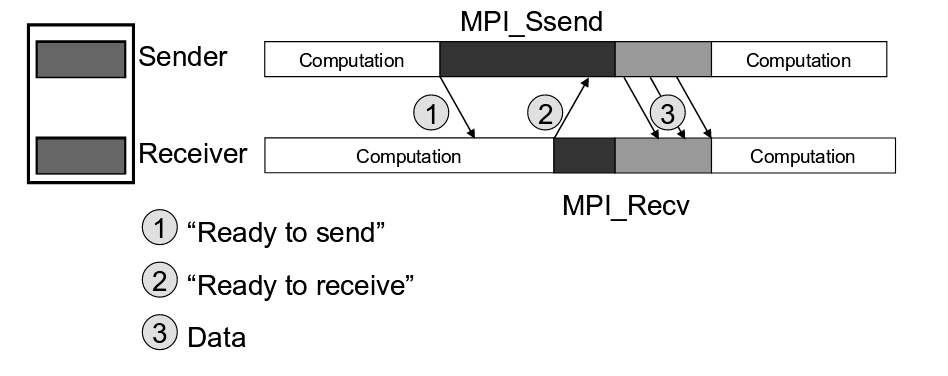
\includegraphics[width=0.9\textwidth]{img/SyncSend_gray.png}
	\subcaption{Ablauf der synchronen Sendeoperation.}
	\label{fig:sync_send}
      \end{subfigure}
      \begin{subfigure}[c]{0.45\textwidth}
	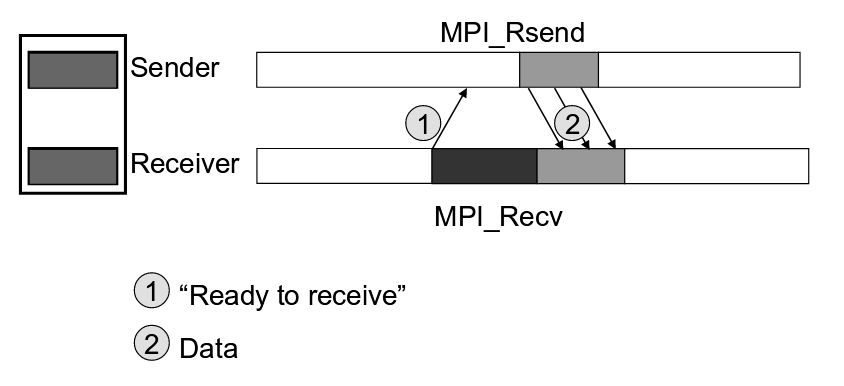
\includegraphics[width=0.9\textwidth]{img/ReadySend_gray.png}
	\subcaption{Ablauf der Ready-Send-Operation.}
	\label{fig:ready_send}
      \end{subfigure}
      \begin{subfigure}[c]{0.5\textwidth}
	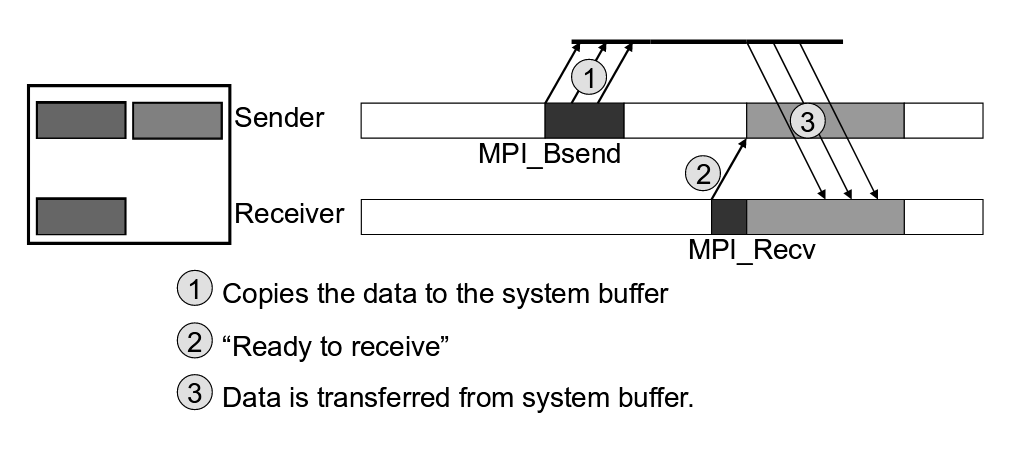
\includegraphics[width=0.9\textwidth]{img/BufferedSend_gray.png}
	\subcaption{Ablauf der gepufferten Sendeoperation.}
	\label{fig:buff_send}
      \end{subfigure}
      \caption{Ablauf unterschiedlicher Kommunikationsmodi in MPI. Quelle: \citet{mpi_p2p}}
      \label{fig:send_var}
    \end{figure}
    
    Beim synchronen Senden wird, wie in \autoref{fig:send_var}\hyperref[fig:sync_send]{.(a)} dargestellt, zunächst vom sendenden Prozess eine ``Ready to send''-Mitteilung verschickt. Auf 
    diese antwortet der empfangende Prozess mit einer ``Ready to receive''-Mitteilung. Im Anschluss findet das Senden und Empfangen der Daten statt. Durch dieses Vorgehen müssen die Prozesse
    aber gegebenenfalls auf einander warten. Die Wartezeit ist in der Abbildung durch die dunkel eingefärbten Bereiche dargestellt. Dafür wird aber nicht nur sichergestellt, dass die gesendeten
    Daten verändert werden dürfen, sondern auch, dass der Empfänger-Prozess zumindest damit begonnen hat die Daten auch zu empfangen. \citep{mpi_p2p, mpiv31}
    
    Das Ready-Send sieht wie eine einfachere synchrone Sende-Variante aus (vgl. \autoref{fig:send_var}\hyperref[fig:ready_send]{.(b)}), ist tatsächlich aber noch restriktiver. Die Methoden \code{MPI\_Rsend}
    beziehungsweise \code{MPI\_Irsend} erwarten, dass die ``Ready to receive''-Mitteilung bereits geschickt wurde, wenn sie aufgerufen werden. Nur wenn diese Mitteilung bereits eingetroffen
    ist, werden die Daten auch gesendet, ansonsten wird ein Fehler gemeldet. Diese Methode soll den System-Overhead durch Sendeoperationen und Synchronisation minimieren. Es wird jedoch 
    dazu geraten diese Methode nur zu verwenden, wenn die zeitliche Abfolge garantiert ist. \citep{mpi_p2p, mpiv31}
    
    Beim Buffered-Send werden die Daten in einem gesonderten Puffer zwischengespeichert. Dies führt durch das zusätzliche Kopieren gegebenenfalls zu weiterem Overhead, dafür kann der 
    Prozess, wie in \autoref{fig:send_var}\hyperref[fig:buff_send]{.(c)} zu erkennen, im Anschluss an den Kopiervorgang seine Arbeit fortsetzen und auch den Sendepuffer bereits verändern. 
    Die eigentliche Sendeoperation wird dann zu einem späteren Zeitpunkt nach der ``Ready to receive''-Mitteilung des Empfängers durchgeführt. Der Puffer zum Zwischenspeichern muss allerdings 
    auch durch den Nutzer zur Verfügung gestellt werden und wird nicht automatisch durch das System verwaltet. \citep{mpi_p2p, mpiv31}
    
    Bei allen blockierenden Methoden können Deadlocks auftreten. Diese können beispielsweise entstehen, wenn zwei Prozesse Daten austauschen wollen, jedoch beide mit einer Sendeoperation
    beginnen, die nicht zurückkehrt, bevor nicht auch das Empfangen der Daten begonnen wurde. Beide Prozesse werden niemals beginnen Daten zu empfangen und werden somit auch
    nie aus dem Senden zurückkehren. Abhilfe können die nicht-blockierenden Methoden liefern.
    
    Die nicht-blockierenden Methoden bestehen grundsätzlich aus zwei Aufrufen. Einer Initialisierung des Sendens/Empfangens, ohne dass auf dessen Ausführung gewartet wird, und
    einer Abschlussmethode, wie \code{MPI\_Wait}, \code{MPI\_Probe} oder \code{MPI\_Test}. Dies nicht-blockierenden Methoden ermöglicht es dem sendenden und dem empfangenden Prozess weitere Arbeiten
    auszuführen, um so möglichst Wartezeiten zu vermeiden beziehungsweise produktiv zu nutzen. Allerdings sollten weder der Sende- noch der Empfangspuffer zwischen Initialisierung und Abschluss
    verändert werden. \citep{mpi_p2p, mpiv31}
    
%     \begin{figure}[p]
%       \begin{subfigure}[c]{0.9\textwidth}
% 	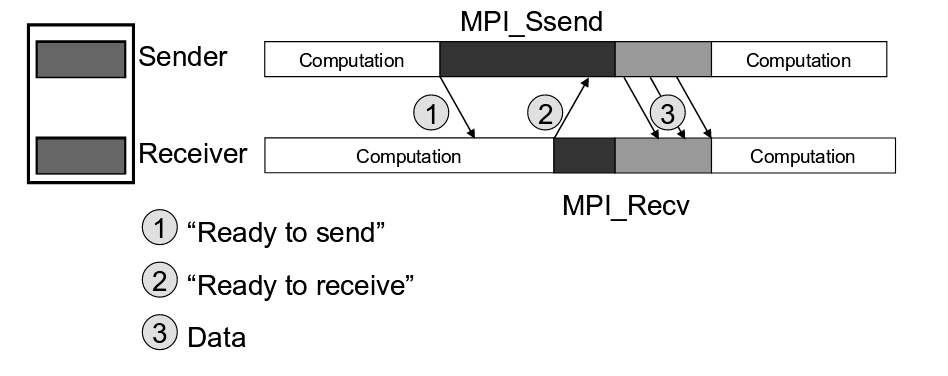
\includegraphics[width=0.9\textwidth]{img/SyncSend_gray.png}
% 	\subcaption{Ablauf der synchronen Sendeoperation.}
% 	\label{fig:sync_send}
%       \end{subfigure}
%       \begin{subfigure}[c]{0.9\textwidth}
% 	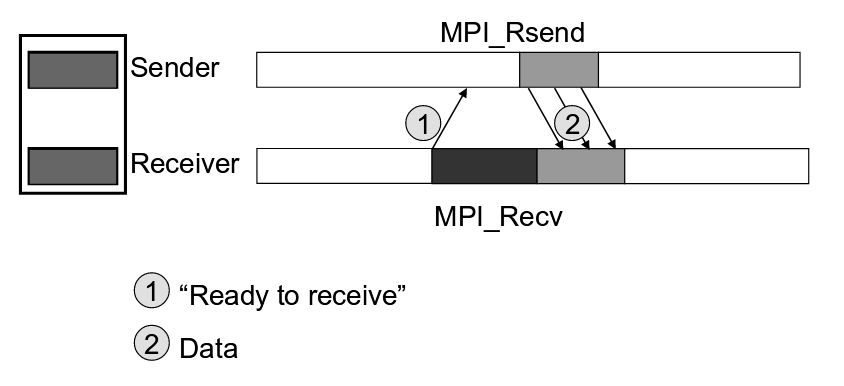
\includegraphics[width=0.9\textwidth]{img/ReadySend_gray.png}
% 	\subcaption{Ablauf der Ready-Send-Operation.}
% 	\label{fig:ready_send}
%       \end{subfigure}
%       \begin{subfigure}[c]{0.9\textwidth}
% 	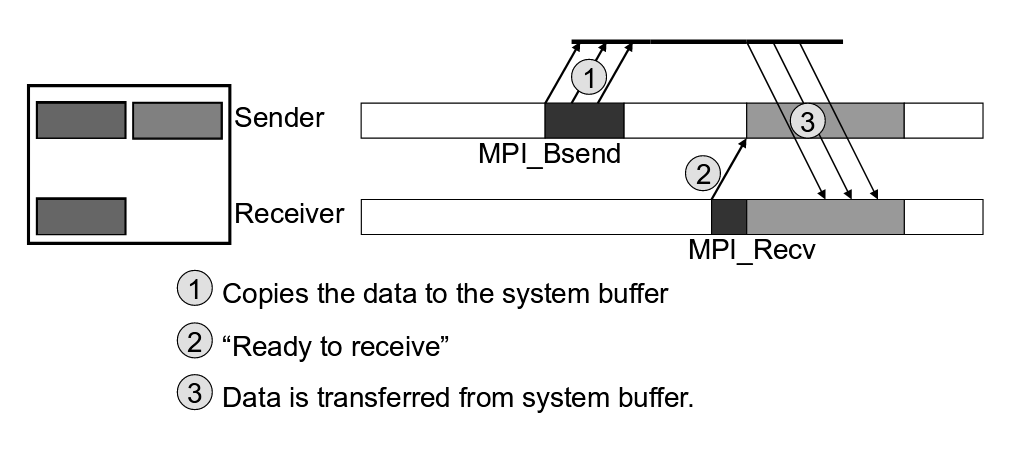
\includegraphics[width=0.9\textwidth]{img/BufferedSend_gray.png}
% 	\subcaption{Ablauf der gepufferten Sendeoperation.}
% 	\label{fig:buff_send}
%       \end{subfigure}
%       \caption{Quelle: \citet{mpi_p2p}}
%       \label{fig:send_var}
%     \end{figure}
%     \clearpage
      
    \subsection{Kollektive Kommunikation}
    \label{sec:kolkom}
    
    \begin{center}
      \begin{figure}[b]
      \centering
      \begin{subfigure}{0.9\textwidth}
      \begin{lstlisting}[language=C, label=lst:bcast, caption={Die Syntax von \code{MPI\_Bcast}}, numbers=none]
	MPI_Bcast(
	  void* data,
	  int count,
	  MPI_Datatype datatype,
	  int root,
	  MPI_Comm communicator)
      \end{lstlisting}
      \end{subfigure}
      \end{figure}
      
      \begin{figure}[b]
	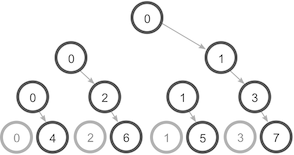
\includegraphics{img/bcast_tree_gray.png}
	\caption{Mögliche Verteilung der Daten durch \code{MPI\_Bcast}. (Quelle: \citet{mpitut})}
	\label{fig:bcast_tree}
      \end{figure}
      \end{center}
      
      Zusätzlich zur klassischen Point-to-Point-Kommuniklation bietet MPI Möglichkeiten für kollektive Kommunikation. Ein Unterschied zur direkten Kommunikation zwischen zwei Knoten ist, dass hier
      keine getrennten Send- und Receive-Operationen durchgeführt werden. Bei der kollektiven Kommunikation rufen alle Prozesse eines Kommunikators dieselbe Methode auf. Daher sind auch die Parameter
      \code{destination} und \code{tag} nicht mehr notwendig. Wie auch bei der Point-to-Point-Kommunikation gibt es bei diesen Methoden jeweils eine blockierende und eine nicht-blockierende Variante.
      
      Die einfachste kollektive Methode ist \code{MPI\_Barrier}. Diese dient nicht dem Austausch von Daten, sondern ausschließlich der  Synchronisation der Prozesse eines Kommunikators.
      Jeder Prozess, der diese Methode aufruft, wartet, bis jeder Prozess des Kommunikators diese Methode ebenfalls aufgerufen hat. Eine Deadlockgefahr besteht, falls nicht alle Prozesse
      des Kommunikators die Methode aufrufen. \citep{mpiv31}
      
      In \autoref{fig:kolkom} sind einige kollektive Methoden und ihre jeweilige Funktionsweise veranschaulicht und werden im Folgenden kurz erläutert.
      
      Der Broadcast dient dazu, Daten von einem Prozess an alle anderen zu verteilen. Die Syntax ist \autoref{lst:bcast} zu finden.

      Die meisten Parameter sind bereits aus dem vorherigen Abschnitt bekannt. Neu ist der Parameter \code{int root}. Dieser bezeichnet den Rang des Prozesses im Kommunikator,
      der die Daten an die anderen verteilen möchte. Er legt also letztlich fest welcher Prozess sendet und welcher empfängt.
      Auch wenn es auf den ersten Blick so aussehen mag, werden die Daten nicht ausschließlich vom Sender nacheinander an alle Empfänger gesendet, was linearen Aufwand
      bedeuten würde, sondern baumartig weitergegeben. In \autoref{fig:bcast_tree} wird ein möglicher Ablauf dargestellt. Durch dieses Vorgehen ist logarithmische Laufzeit erreichbar. 
      \citep{mpitut, mpiv31}
      
      \code{MPI\_Scatter} dient ebenfalls dem Verteilen von Daten von einem Prozess auf die anderen, jedoch wird hier ein Array auf alle Prozesse eines Kommunikators verteilt.
      Dies kann zum Beispiel genutzt werden, um Testdaten in einem Root-Prozess einzulesen und dann an die anderen Prozesse zu verteilen. Umgekehrt zieht \code{MPI\_Gather} die
      Daten aller Prozesse eines Kommunikators auf einem Prozess zusammen, beispielsweise um die Ergebnisse einer verteilten Berechnung auf einem Prozess zu aggregieren und
      auszugeben. Beim darunter abgebildeten \code{MPI\_Allgather} wird das Ergebnis nicht nur auf einem, sondern auf allen Prozessen gesammelt. \citep{mpitut, mpiv31}
      
      Ähnlich zu den beiden Gather-Methoden sind die Methoden \code{MPI\_Reduce} und \code{MPI\_\-Allreduce}. Auch diese sammeln Daten von allen Prozessen auf einen, respektive
      auf alle Prozesse, zusammen. Jedoch werden hierbei die Daten nicht einfach in einem Array gebündelt, sondern über den Parameter \code{MPI\_Op op} eine Operation mitgegeben,
      die auf die gesammelten Daten angewandt wird. So können aus den gesendeten Daten direkt das Maximum, Minimum, die Summe und vieles mehr bestimmt werden. \citep{mpitut, mpiv31}
      
      Zuletzt ist \code{MPI\_Alltoall} in \autoref{fig:kolkom} dargestellt. Hierbei führt quasi jeder Prozess ein Scatter durch. Man könnte es auch als \textit{Transponieren} der
      ``Prozess-Daten-Matrix'' bezeichnen. \citep{mpiv31}
      
      Von jeder dieser kollektiven Methoden gibt es wie bereits erwähnt ebenfalls eine nicht-blockierende Variante, die, der Namenskonvention folgend, durch ein eingeschobenes \code{I}
      gekennzeichnet ist. 
      
      \begin{figure}[b]
      \begin{subfigure}{0.9\textwidth}
      \begin{lstlisting}[language=C, label=lst:a2a, caption={Die Syntax von \code{MPI\_Alltoallv}}, numbers=none]
	int MPI_Alltoallv(
	  const void* sendbuffer,
	  const int sendcounts[], 
	  const int senddispls[], 
	  MPI_Datatype sendtype, 
	  void* recvbuffer, 
	  const int recvcounts[], 
	  const int recvdispls[], 
	  MPI_Datatype recvtype, 
	  MPI_Comm comm)
      \end{lstlisting}
      \end{subfigure}
      \end{figure}
      
      Außerdem gibt es für die Daten austauschenden Methoden eine \textit{vektorisierte} Variante. Alle zuvor erläuterten Methoden erwarten eine feste Anzahl an zu 
      kommunizierenden Elementen pro Prozess.
      Es kann aber vorkommen, dass zwischen unterschiedlichen Prozessen unterschiedliche Anzahlen von Elementen ausgetauscht werden müssen. Genau dies ist durch die vektorisierten Varianten, 
      zu erkennen an einem hinter dem Namen angefügten \code{v}, möglich. Diese erwarten jeweils ein Array von Anzahlen zu sendender und zu empfangender Elemente.
      Als Beispiel ist die Syntax der vektorisierten Alltoall-Methode in \autoref{lst:a2a} aufgeführt.
      
      Für $i \in \nullhaken{p-1}$ legt der $i$-te Eintrag der Arrays \code{sendcounts} und \code{recvcounts} fest, wie viele Elemente an den $i$-ten Prozess gesendet, respektive vom $i$-ten
      Prozess empfangen werden. Neu sind außerdem die \code{int}-Arrays \code{senddispls} und \code{recvdispls}. Der $i$-te Eintrag legt hier fest, ab welchem Index die Daten im 
      \code{sendbuffer} für den $i$-ten Prozess bestimmt sind, beziehungsweise ab welchem Index im \code{recvbuffer} die Daten des $i$-ten Prozesses zu empfangen sind. \citep{mpiv31}


      \begin{figure}[tbp]%
      \begin{subfigure}[l]{0.87\textwidth}
	\begin{tabular}[]{m{0.2cm} m{0.3cm}|m{0.3cm}|m{0.3cm}|m{0.3cm}|m{0.3cm}|m{0.3cm} m{1.5cm} m{0.3cm}|m{0.3cm}|m{0.3cm}|m{0.3cm}|m{0.3cm}|m{0.3cm}}
	  & \multicolumn{13}{l}{Daten $\longrightarrow$}\\
	  \cline{2-7} \cline{9-14}
	  \multirow{6}{*}{\begin{turn}{-90} Prozesse $\longrightarrow$ \end{turn}}
	  &\multicolumn{1}{|c|}{$A_0$}& & & & &\multicolumn{1}{|m{0.3cm}|}{ } &\multirow{6}{*}{\large $\xrightarrow{\text{Broadcast}}$} & \multicolumn{1}{|c|}{$A_0$}& & & & &\multicolumn{1}{|m{0.3cm}|}{ }\\
	  \cline{2-7} \cline{9-14}
	  &\multicolumn{1}{|c|}{ }& & & & &\multicolumn{1}{|c|}{ }                         & & \multicolumn{1}{|c|}{$A_0$}    & & & & &                \multicolumn{1}{|c|}{ }    \\
	  \cline{2-7} \cline{9-14}
	  &\multicolumn{1}{|c|}{ }& & & & &\multicolumn{1}{|c|}{ }                         & & \multicolumn{1}{|c|}{$A_0$}    & & & & &                \multicolumn{1}{|c|}{ }    \\
	  \cline{2-7} \cline{9-14}
	  &\multicolumn{1}{|c|}{ }& & & & &\multicolumn{1}{|c|}{ }                         & & \multicolumn{1}{|c|}{$A_0$}    & & & & &                \multicolumn{1}{|c|}{ }    \\
	  \cline{2-7} \cline{9-14}
	  &\multicolumn{1}{|c|}{ }& & & & &\multicolumn{1}{|c|}{ }                         & & \multicolumn{1}{|c|}{$A_0$}    & & & & &                \multicolumn{1}{|c|}{ }    \\
	  \cline{2-7} \cline{9-14}
	  &\multicolumn{1}{|c|}{ }& & & & &\multicolumn{1}{|c|}{ }                         & & \multicolumn{1}{|c|}{$A_0$}    & & & & &                \multicolumn{1}{|c|}{ }    \\
	  \cline{2-7} \cline{9-14}
	\end{tabular}
	\subcaption{Beim \code{MPI\_Bcast} wird ein Datensatz von einem Root-Prozess an alle anderen Prozesse gesendet und von diesen empfangen.}
      \end{subfigure}
      
      \begin{subfigure}[l]{0.87\textwidth}
	\begin{tabular}[]{m{0.2cm} m{0.3cm}|m{0.3cm}|m{0.3cm}|m{0.3cm}|m{0.3cm}|m{0.3cm} m{1.5cm} m{0.3cm}|m{0.3cm}|m{0.3cm}|m{0.3cm}|m{0.3cm}|m{0.3cm}}
	  & \multicolumn{13}{l}{Daten $\longrightarrow$}\\
	  \cline{2-7} \cline{9-14}
	  \multirow{6}{*}{\begin{turn}{-90} Prozesse $\longrightarrow$ \end{turn}}
	  &\multicolumn{1}{|c|}{$A_0$}&$A_1$&$A_2$&$A_3$&$A_4$&\multicolumn{1}{|m{0.3cm}|}{$A_5$} &\multirow{6}{*}{\large \shortstack{ $\xrightarrow{\text{ Scatter }}$ \\ $\xleftarrow[\text{ Gather }]{}$ }} & \multicolumn{1}{|c|}{$A_0$}& & & & &\multicolumn{1}{|m{0.3cm}|}{ }\\
	  \cline{2-7} \cline{9-14}
	  &\multicolumn{1}{|c|}{ }& & & & &\multicolumn{1}{|c|}{ }                         & & \multicolumn{1}{|c|}{$A_1$}    & & & & &                \multicolumn{1}{|c|}{ }    \\
	  \cline{2-7} \cline{9-14}
	  &\multicolumn{1}{|c|}{ }& & & & &\multicolumn{1}{|c|}{ }                         & & \multicolumn{1}{|c|}{$A_2$}    & & & & &                \multicolumn{1}{|c|}{ }    \\
	  \cline{2-7} \cline{9-14}
	  &\multicolumn{1}{|c|}{ }& & & & &\multicolumn{1}{|c|}{ }                         & & \multicolumn{1}{|c|}{$A_3$}    & & & & &                \multicolumn{1}{|c|}{ }    \\
	  \cline{2-7} \cline{9-14}
	  &\multicolumn{1}{|c|}{ }& & & & &\multicolumn{1}{|c|}{ }                         & & \multicolumn{1}{|c|}{$A_4$}    & & & & &                \multicolumn{1}{|c|}{ }    \\
	  \cline{2-7} \cline{9-14}
	  &\multicolumn{1}{|c|}{ }& & & & &\multicolumn{1}{|c|}{ }                         & & \multicolumn{1}{|c|}{$A_5$}    & & & & &                \multicolumn{1}{|c|}{ }    \\
	  \cline{2-7} \cline{9-14}
	\end{tabular}
	\subcaption{\code{MPI\_Scatter} verteilt ein Array von Daten auf die Prozesse. \code{MPI\_Gather} vereinigt Daten aller Prozesse in einem Array auf einem Root-Prozess.}
      \end{subfigure}
      
      \begin{subfigure}[l]{0.87\textwidth}
	\begin{tabular}[]{m{0.2cm} m{0.3cm}|m{0.3cm}|m{0.3cm}|m{0.3cm}|m{0.3cm}|m{0.3cm} m{1.5cm} m{0.3cm}|m{0.3cm}|m{0.3cm}|m{0.3cm}|m{0.3cm}|m{0.3cm}}
	  & \multicolumn{13}{l}{Daten $\longrightarrow$}\\
	  \cline{2-7} \cline{9-14}
	  \multirow{6}{*}{\begin{turn}{-90} Prozesse $\longrightarrow$ \end{turn}}
	  &\multicolumn{1}{|c|}{$A_0$}&$B_0$&$C_0$&$D_0$&$E_0$&\multicolumn{1}{|m{0.3cm}|}{$F_0$} &\multirow{6}{*}{\large $\xleftarrow{\text{Allgather}}$} & \multicolumn{1}{|c|}{$A_0$}& & & & &\multicolumn{1}{|m{0.3cm}|}{ }\\
	  \cline{2-7} \cline{9-14}
	  &\multicolumn{1}{|c|}{$A_0$}&$B_0$&$C_0$&$D_0$&$E_0$&\multicolumn{1}{|m{0.3cm}|}{$F_0$}                         & & \multicolumn{1}{|c|}{$B_0$}& & & & &\multicolumn{1}{|c|}{ }\\
	  \cline{2-7} \cline{9-14}
	  &\multicolumn{1}{|c|}{$A_0$}&$B_0$&$C_0$&$D_0$&$E_0$&\multicolumn{1}{|m{0.3cm}|}{$F_0$}                         & & \multicolumn{1}{|c|}{$C_0$}& & & & &\multicolumn{1}{|c|}{ }\\
	  \cline{2-7} \cline{9-14}
	  &\multicolumn{1}{|c|}{$A_0$}&$B_0$&$C_0$&$D_0$&$E_0$&\multicolumn{1}{|m{0.3cm}|}{$F_0$}                         & & \multicolumn{1}{|c|}{$D_0$}& & & & &\multicolumn{1}{|c|}{ }\\
	  \cline{2-7} \cline{9-14}
	  &\multicolumn{1}{|c|}{$A_0$}&$B_0$&$C_0$&$D_0$&$E_0$&\multicolumn{1}{|m{0.3cm}|}{$F_0$}                         & & \multicolumn{1}{|c|}{$E_0$}& & & & &\multicolumn{1}{|c|}{ }\\
	  \cline{2-7} \cline{9-14}
	  &\multicolumn{1}{|c|}{$A_0$}&$B_0$&$C_0$&$D_0$&$E_0$&\multicolumn{1}{|m{0.3cm}|}{$F_0$}                         & & \multicolumn{1}{|c|}{$F_0$}& & & & &\multicolumn{1}{|c|}{ }\\
	  \cline{2-7} \cline{9-14}
	\end{tabular}
	\subcaption{\code{MPI\_Allgather} vereint ebenfalls Daten aller Prozesse, allerdings erhält jeder Prozess eine Kopie des Arrays.}
      \end{subfigure}
      
      \begin{subfigure}[l]{0.87\textwidth}
	\begin{tabular}[]{m{0.2cm} m{0.3cm}|m{0.3cm}|m{0.3cm}|m{0.3cm}|m{0.3cm}|m{0.3cm} m{1.5cm} m{0.3cm}|m{0.3cm}|m{0.3cm}|m{0.3cm}|m{0.3cm}|m{0.3cm}}
	  & \multicolumn{13}{l}{Daten $\longrightarrow$}\\
	  \cline{2-7} \cline{9-14}
	  \multirow{6}{*}{\begin{turn}{-90} Prozesse $\longrightarrow$ \end{turn}}
	  &\multicolumn{1}{|c|}{$A_0$}&$A_1$&$A_2$&$A_3$&$A_4$&\multicolumn{1}{|m{0.3cm}|}{$A_5$} &\multirow{6}{*}{\large $\xrightarrow{\text{Alltoall}}$} & \multicolumn{1}{|c|}{$A_0$}&$B_0$&$C_0$&$D_0$&$E_0$&\multicolumn{1}{|m{0.3cm}|}{$F_0$}\\
	  \cline{2-7} \cline{9-14}
	  &\multicolumn{1}{|c|}{$B_0$}&$B_1$&$B_2$&$B_3$&$B_4$&\multicolumn{1}{|m{0.3cm}|}{$B_5$} & & \multicolumn{1}{|c|}{$A_1$}&$B_1$&$C_1$&$D_1$&$E_1$&\multicolumn{1}{|m{0.3cm}|}{$F_1$}\\
	  \cline{2-7} \cline{9-14}
	  &\multicolumn{1}{|c|}{$C_0$}&$C_1$&$C_2$&$C_3$&$C_4$&\multicolumn{1}{|m{0.3cm}|}{$C_5$} & & \multicolumn{1}{|c|}{$A_2$}&$B_2$&$C_2$&$D_2$&$E_2$&\multicolumn{1}{|m{0.3cm}|}{$F_2$}\\
	  \cline{2-7} \cline{9-14}
	  &\multicolumn{1}{|c|}{$D_0$}&$D_1$&$D_2$&$D_3$&$D_4$&\multicolumn{1}{|m{0.3cm}|}{$D_5$} & & \multicolumn{1}{|c|}{$A_3$}&$B_3$&$C_3$&$D_3$&$E_3$&\multicolumn{1}{|m{0.3cm}|}{$F_3$}\\
	  \cline{2-7} \cline{9-14}
	  &\multicolumn{1}{|c|}{$E_0$}&$E_1$&$E_2$&$E_3$&$E_4$&\multicolumn{1}{|m{0.3cm}|}{$E_5$} & & \multicolumn{1}{|c|}{$A_4$}&$B_4$&$C_4$&$D_4$&$E_4$&\multicolumn{1}{|m{0.3cm}|}{$F_4$}\\
	  \cline{2-7} \cline{9-14}
	  &\multicolumn{1}{|c|}{$F_0$}&$F_1$&$F_2$&$F_3$&$F_4$&\multicolumn{1}{|m{0.3cm}|}{$F_5$} & & \multicolumn{1}{|c|}{$A_5$}&$B_5$&$C_5$&$D_5$&$E_5$&\multicolumn{1}{|m{0.3cm}|}{$F_5$}\\
	  \cline{2-7} \cline{9-14}
	\end{tabular}
	\subcaption{\code{MPI\_Alltoall} ist ein simultanes MPI\_Scatter aller Prozesse. Betrachtet man die Prozesse und Daten als Matrix, wird eine Matrixtranformation durchgeführt.}
      \end{subfigure}
      
      \caption{Möglichkeiten der kollektiven Kommunikation in MPI. (Quelle: \citet{dartmouth})}%
      \label{fig:kolkom}%
\end{figure}%%      
      \clearpage
      
      

  %Bereits in \autoref{sec:mot} wurde gezeigt, dass das Problem der gravitationellen Wechselwirkungen in unserer Galaxie mit einem aktuellen Computer nicht ohne 
    weiteres lösbar ist. 
    Konnten sich früher Programmierer darauf verlassen, dass in einigen Jahren eine deutlich schnellere Prozessorgeneration erscheinen würde, so dass Probleme ohne 
    weitere Änderungen schneller gelöst werden könnten, ist dies heute leider nicht mehr der Fall. 
    
    Grund hierfür ist die Physik. Dazu ein kleines Rechenexperiment: Nehmen wir einen Prozessorchip von etwa einem Zentimeter Durchmesser an und vergegenwärtigen wir 
    uns die Lichtgeschwindigkeit $c \approx 3\cdot10^{10}$ \footnote{Bureau International des Poids et Mesures [1975], \textit{Resolution 2 of the 15th CGPM},\\URL:
    https://www.bipm.org/en/CGPM/db/15/2/ Abgerufen am 16.07.2018}. Licht könnte diesen Chip also etwa 30 Milliarden mal pro Sekunde durchqueren, was 30 Gigahertz
    entspräche. Bedenkt man, dass man in Prozessoren mit Elektrizität arbeitet und somit beispielsweise mit kapazitären Effekten und proportional zur Taktfrequenz steigender
    Verlustleistung zu kämpfen hat, sind die 3 Gigahertz aktueller Mittelklasseprozessoren durchaus nicht zu verachten.
    
    Zwar wäre eine Möglichkeit die Chips weiter zu verkleinern, jedoch machen dem Fortschritt hier quantenmechanische Phänomene aktuell noch einen Strich durch die Rechnung.
    Ein gängiger und gangbarer Lösungsweg besteht in der Parallelisierung von Soft- und Hardware. Durch das gleichmäßige Verteilen eines Algorithmus auf mehrere Prozessoren
    kann die Gesamtlaufzeit entsprechend verringert werden. Unter optimalen Bedingungen könnte theoretisch eine Verdopplung der Prozessoranzahl eine Halbierung der Laufzeit
    bewirken. Heute haben daher die meisten Prozessoren nicht mehr nur einen Rechenkern, sondern mehrere und für die Berechnung großer mathematischer Probleme arbeiten oft viele
    Rechner zusammen an der Lösung. \citep{hpcskript}
    
    Ein weiterer Grund für parallele beziehungsweise verteilte Rechnersysteme ist die Diskrepanz zwischen vorhandenem und benötigtem Speicher. Beispielsweise hat der diesbezüglich größte
    Computer im Rechenzentrum der Christian-Albrecht-Universität Kiel einen Hauptspeicher von 768 GB. Ein aktuelles, speicherintensives Problem ist ein engmaschiges 
    Klimamodell der Erde. Bei einer Dichte von einer Masche alle 1,56 km in Äquatornähe wird der Gesamtspeicherbedarf auf etwa 24000 GB geschätzt \citep{climate}. Ein Problem
    dieser Größe passt nicht mehr in den Hauptspeicher eines Computers.
    Hinzu kommt die Skalierbarkeit solcher Probleme: Angenommen ein Hauptspeicher von 24000 GB stünde auf einem Computer zur Verfügung. Warum bei einer Maschendichte von 
    1,56 km stehen bleiben und nicht noch feiner auflösen um noch genauere Berechnungen durchzuführen?
    Warum bei der Berechnung der gravitationellen Wechselwirkungen bei den Sonnen unserer Galaxie stehen bleiben und nicht die Planeten, Monde oder noch kleinere Himmelskörper mit einbeziehen? 
    Diese Probleme, und damit auch der Speicherbedarf, lassen sich also nahezu beliebig vergrößern. Wir benötigen also eine Möglichkeit, günstig genügend Hauptspeicher zur Verfügung zu stellen.
    Das Vernetzen von Computern und das Verteilen der Arbeit und der Daten durch parallel arbeitende Algorithmen auf die vernetzten Rechner ist ein Lösungsansatz für dieses Problem.
    
    Im folgenden Kapitel wird kurz skizziert, wie parallel arbeitende Hardware gestaltet sein kann und welche Vor- und Nachteile und welche Herausforderungen damit einhergehen. Grundbegriffe
    der Computerarchitektur werden vorausgesetzt, da eine Einführung den Umfang dieser Arbeit sprengen würde.
    
    \subsection{Parallele Hardware}
    \label{sec:parhard}
      \subsubsection{Prozessor}
      \label{sec:processor}
      \citet{flynn} klassifiziert vier unterschiedliche Architekturen von Rechnern. Dabei unterteilt er nach der Möglichkeit des Prozessors, zu einem Zeitpunkt einzelne oder mehrere
      Instruktionen beziehungsweise Datensätze zu verarbeiten (vgl. \autoref{tab:flynn}).
      \begin{table}[tb]
	\centering
	\begin{tabular}{|p{3.5cm}|p{4cm}|p{4cm}|}
	  \hline
			                             & eine Instruktion \newline (single instruction)       & mehrere Instruktionen \newline (multiple instruction) \\
	  \hline
	  ein Datensatz \newline (single data)       & SISD: konventioneller \newline einkerniger Prozessor & MISD: Spezialrechner                                  \\
	  \hline
	  mehrere Datensätze \newline (multiple data)& SIMD: Vektorrechner                                  & MIMD: Multicore; \newline Clustersystem               \\
	  \hline
	\end{tabular}
	\caption{Flynnsche Klassifikation mit Beispielen.}
	\label{tab:flynn}
      \end{table}
      
      Vor einigen Jahrzehnten waren die meisten Prozessoren in PCs noch SISD-Architekturen. Sie hatten einen Prozessor mit einem einzelnen Kern; konnten also zu jedem Zeitpunkt nur eine Instruktion
      auf einem Datensatz ausführen. Heute sind Multicore-Prozessoren üblich. Auf einem Prozessorchip finden sich hierbei mehrere Rechenkerne. Die einzelnen Kerne sind unabhängig voneinander; sie 
      verwalten eigene Register und führen eigene Instruktionen aus. Daher zählen Multicore-Prozessoren zu den MIMD-Architekturen. Zu diesen Architekturen gehören ebenfalls die später erläuterten 
      \hyperref[sec:netzwerk]{Clustersysteme}. \citep{flynn, multicore}
      
      MIMD-Architekturen sind auf Grund ihrer autonom arbeitenden und programmierbaren Prozessoren sehr flexibel und können viele Probleme effizient lösen. Die Autonomie der Prozessoren
      stellt die Programmierung aber auch vor Herausforderungen. Durch die asynchrone Ausführung der Programme wird das Verhalten des gesamten Systems schwer vorhersagbar. \citep{hpcskript}
      
      MISD-Architekturen, also solche, in denen parallel auf einem Datum mehrere Instruktionen ausgeführt werden können, sind nur in Spezialrechnern zu finden und für die Lösung der meisten
      Probleme nicht geeignet. \citep{architect, korbler}
      
      SIMD-Architekturen hingegen, in denen auf mehreren Daten parallel die gleiche Instruktion ausgeführt werden kann, sind durchaus gängig.
      Ihr Hintergrund sind Algorithmen, die auf ganzen Reihen von Daten immer wieder dieselbe Operation ausführen. Während beim Ansatz der MIMD-Architekturen die Operationen dynamisch auf die
      einzelnen Recheneinheiten verteilt werden, ist der Ansatz von SIMD-Architekturen beziehungsweise von Vektorrechnern, die Anzahl der Rechenwerke in den Recheneinheiten zu erhöhen 
      und eine Operation für mehrere Daten gleichzeitig auszuführen. Zum Beispiel werden für die Berechnung der Gravitationskräfte für viele Körper immer wieder dieselben Operationen 
      verarbeitet. Anstatt diese also für jedes einzelne Paar von Körpern durchzuführen, könnten sie für mehrere Paare von Körpern gleichzeitig durchgeführt werden.
      
      Der Name ``Vektorrechner'' leitet sich von der Anlehnung an die kartesische Geometrie her, in der ein Vektor ein Tupel von Zahlen ist. Entsprechend werden Daten desselben Typs ebenfalls 
      als Vektoren bezeichnet. Um solche Vektoren handhaben zu können, verfügen Vektorrechner über spezielle Vektorregister, die mehrere Daten gleichzeitig fassen können. Für jedes einzelne
      Datum innerhalb dieser Register ist dann jeweils ein eigenes Rechenwerk im Kern zuständig. \citep{hpcskript}
      
      Prozessoren laden in der Regel nicht nur ein einzelnes Datum, sondern gleich eine sogenannte \textit{cache line} aus dem Hauptspeicher. Daher ist es sinnvoll, 
      um SIMD-Parallelisierung optimal ausnutzen zu können, die Daten im Hauptspeicher anhand dieser cache lines anzuordnen. Dazu müssen in der Regel explizite Methoden zum Anfordern von 
      \wlabel{\textit{aligned memory}}{w:aligned} verwendet werden. Außerdem müssen die parallel zu verarbeitenden Daten im Hauptspeicher direkt hintereinander und nicht durch andere Daten 
      unterbrochen auftauchen. Nehmen wir an, wir wollten die Daten der Körper, die für die Berechnung der Gravitationskräfte benötigt werden, in einer Struktur zusammenfassen. Wollen wir
      Daten zu vielen dieser Körper speichern, so wäre es in Bezug auf Vektorrechner nicht sinnvoll, ein Array dieser Strukturen anzulegen (engl.: \wlabel{\textit{array of structs}}{w:aos}).
      Dabei würden die im Sinne der Vektorisierung zusammengehörigen Daten durch andere getrennt. Um eine Vektorisierung zu ermöglichen, ist es daher sinnvoll die Struktur so zu definieren,
      dass sie Arrays der benötigten Daten beinhaltet (engl.: \wlabel{\textit{struct of arrays}}{w:soa}). So kann sichergestellt werden, dass diese Daten im Hauptspeicher hintereinander stehen.
      \citep{hpcskript, architect}
      
      Viele aktuelle Multicore-Prozessoren verfügen zusätzlich über einige Möglichkeiten der Vektorisierung. Es existieren aber auch auf diese Art der Parallelisierung spezialisierte Prozessoren.
      \citep{architect}
      
      \subsubsection{Speicherverwaltung}
      \label{sec:speicher}
	In \autoref{sec:parrech} wurde bereits kurz erwähnt, dass bei Multicore-Prozessoren jeder Kern seine eigenen Register hat. Genau genommen verfügen die Kerne meist auch über privaten L1-,
	seltener über L2- oder L3-Cache. Diese sind meist \textit{shared} (dt.: gemeinsam genutzt). Shared Memory wird von allen Prozessoren gemeinsam verwaltet.
	
	Grundsätzlich können die heute üblichen MIMD Architekturen weiter anhand ihrer Speicherverwaltung unterteilt werden. Beim Shared-Memory-Modell wird ein globaler
	Speicher gemeinsam genutzt. Sie teilen sich also einen gemeinsamen Adressraum. Dies trifft in der Regel auf den Hauptspeicher, aber eventuell auch auf ebenen des Caches zu.
	Anders ist dies beim Distributed-Memory-Modell. Hier besitzt jeder Prozessor seinen eigenen Speicher. Distributed-Memory-Systeme sind in der Regel vernetzte Rechnersysteme. Allerdings wird
	auch auf Shared-Memory-Systemen durch moderne Betriebssysteme ein Distributed-Memory-Modell simuliert. Durch die Virtualisierung des Hauptspeichers etwa wird jedes Programm behandelt,
	als hätte es den Hauptspeicher für sich alleine. Dabei wird jedem Programm ein privater Bereich des Hauptspeichers zugewiesen. Das Programm nutzt diesen Bereich, als sei es der gesamte
	Hauptspeicher. \citep{korbler}
	
	Der Vorteil von gemeinsam genutztem Speicher ist, vorausgesetzt das Programm wurde entsprechend entworfen, dass die Ergebnisse eines Kerns den anderen automatisch auch zur Verfügung stehen. 
	Arbeiten  also mehrere Recheneinheiten gemeinsam an einem Problem, müssen die Ergebnisse einer Einheit den anderen also gegebenenfalls nicht explizit mitgeteilt werden. Dies vermeidet Overhead
	durch das Austauschen und Kopieren von Daten.
	Jedoch ist es bei privatem Cache möglich, diesen in größerer Nähe zum zugehörigen Kern auf dem Chip zu platzieren. Dies führt zu besseren Zugriffszeiten als gänzlich gemeinsam genutzter 
	Cache und wird daher auch oft verwendet. 
	
	Ein Nachteil von Shared-Memory-Systemen ist, dass der Schaltungsaufwand für den Zugriff auf den gemeinsam genutzten Speicher mit wachsender Anzahl Recheneinheiten rapide ansteigt
	\citep{hpcskript}. Außerdem können Race Conditions auftreten, die durch den gemeinsam genutzten Speicher verursacht werden. Diese können dazu führen, dass die Ergebnisse von Programmen
	unvorhersagbar werden.
	
	Beim Schreiben von parallelen Programmen ist also besondere Vorsicht geboten. Gegebenenfalls müssen Zugriffe auf gemeinsam genutzte Ressourcen zeitweise unterbunden werden, um Race Conditions
	zu vermeiden. Außerdem muss klar sein, welche Daten sich wo befinden, und ob sie gemeinsam genutzt werden oder nicht. Dies ist gegebenenfalls eine noch größere Herausforderung, wenn der Hauptspeicher 
	innerhalb eines parallelen Programms teilweise gemeinsam genutzt wird und teilweise verteilt ist.
	
      \subsubsection{Netzwerk}
      \label{sec:netzwerk}
		
	Wie bereits erwähnt gibt es Probleme, die für einen einzelnen Computer zu viel Hauptspeicher benötigen oder zu viel Rechenaufwand bedeuten. Daher ist es naheliegend, Computer zu Netzwerken,
	sogenannten \textit{Clustersystemen}, zusammenzuschließen. Hierbei können die vernetzten Computer, die als \textit{Knoten} des Clustersystems bezeichnet werden, über die 
	Netzwerkverbindung kommunizieren. Clustersysteme gehören zur Klasse der MIMD-Architekturen und stellen meist eine Mischform aus Distributed- und Shared-Memory-Modell dar: Jeder Knoten hat 
	seinen eigenen Hauptspeicher, der nicht mit den anderen Knoten geteilt wird; die einzelnen Knoten sind in der Regel aber Shared-Memory-Systeme. Meist verfügen die einzelnen Knoten über
	einen oder mehrere Multicore-Prozessor(en). \citep{cluster}
	
    \subsection{Parallele Software}
      Im vorherigen Abschnitt wurde die Entwicklung von einzelnen Computern mit einer Recheneinheit hin zu Clustersystemen skizzert, deren Knoten mit multiplen Recheneinheiten bestückt sind.
      
      Solange es sich um einen Computer mit Multicore-Prozessor handelt, ist bis dato keine Änderung an der Software notwendig, um auf diesem Multicore-Prozessor lauffähig zu sein. 
      Auf einem Computer läuft in der Regel nicht nur ein einzelnes Programm, sondern mindestens noch ein Betriebssystem und meist auch noch einige weitere Programme.
      Der Prozessor kann nun lediglich mehrere Programme echt parallel verarbeiten.
      
      Allerdings profitiert ein Programm bis dato noch wenig von parallel arbeitender Technologie; es wird nur gegebenenfalls seltener von anderen Programmen unterbrochen.
      Soll sich das Potential der Parallelität für ein Programm voll entfalten, so muss das Programm selbst parallel arbeiten, um so mehrere Kerne beziehungsweise mehrere Knoten eines 
      Clusters nutzen zu können. 
      
      Dazu sind natürlich auch entsprechende Entwicklungen im Bereich der Software notwendig. Zum einen muss es überhaupt möglich sein, mehrere Instanzen eines 
      Prozesses zu starten und diese zusammenarbeiten zu lassen. Dies impliziert aber wiederum die Schaffung von Möglichkeiten, die oben erwähnten Race Conditions zu vermeiden. Schließlich 
      müssen für Programme, die auf Clustersystemen arbeiten, Möglichkeiten geschaffen werden zu kommunizieren. Durch diese Kommunikation wäre es dann auch nicht mehr notwendig, alle Daten
      lokal abrufbar zu haben. Stattdessen wäre es möglich, die Datenmenge auf die Knoten zu verteilen und bei Bedarf zwischen Knoten auszutauschen. Erst dadurch sind Probleme wie die 
      Berechnung der Gravitationskräfte oder engmaschige Klimamodelle zu bewältigen.
      All diese Konzepte vorzustellen wäre im Rahmen dieser Arbeit nicht zielführend. Wir beschränken uns also auf die Einführung eines Konzeptes.
      
      \subsubsection{Das Message-Passing-Modell}
      \label{sec:mpm}
%       \begin{figure}[bt]%
% 	\centering%
% 	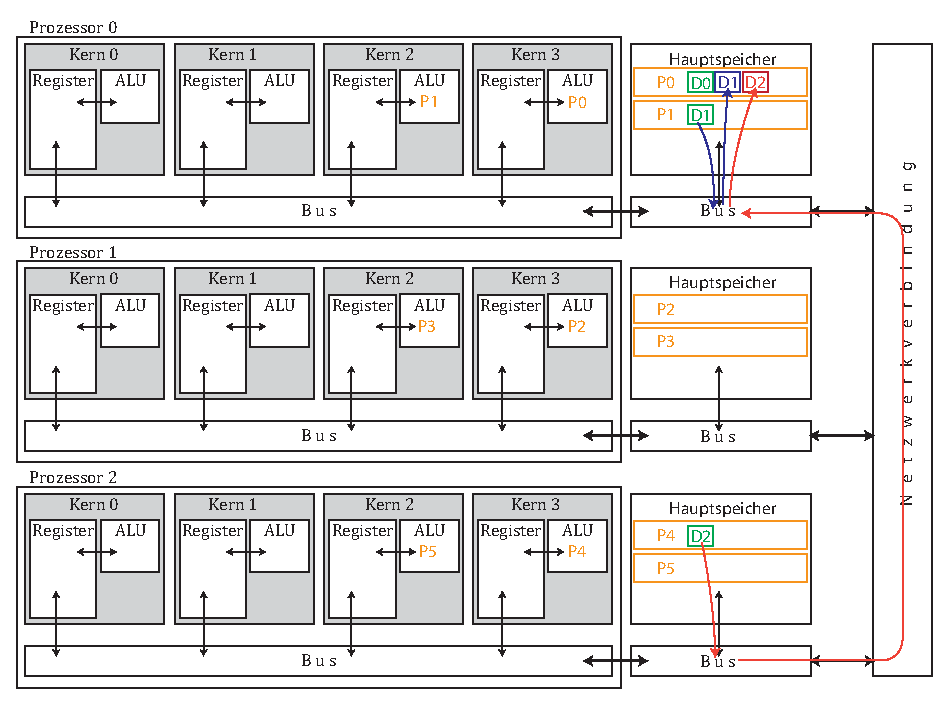
\includegraphics[width=0.9\textwidth]{img/multicorecluster_com.eps}%
% 	\caption{Eine Veranschaulichung des Message-Passings auf einem Clustersystem. In rot die Kommunikation zwischen zwei Knoten eines Clustersystems, in blau die Kommunikation innerhalb
% 	eines Knotens.}%
% 	\label{fig:message-passing}%
%       \end{figure}%
      Für unser Beispielproblem der Berechnung der Gravitationskräfte ist ein Programm vonnöten, das auf einem Clustersystem läuft und dessen Speicher verteilt verwaltet wird.
      Daher wird im folgenden Kapitel ein Parallel-Programing-Modell vorgestellt, das die Schwierigkeiten von Shared-Memory-Systemen umgeht und ein Konzept der Speicherverwaltung 
      und Kommunikation auf verteilten Rechnersystemen liefert.
      Dieses Konzept ist das sogenannte \textit{Message-Passing-Modell}. 
      Dieses Modell geht von einer Menge von \textit{autonomen} Prozessen aus, die
      \begin{enumerate}
       \item eindeutig benannt sind und
       \item jeweils über \textit{privaten Speicher} verfügen.
      \end{enumerate}
      Dies spezifiziert nicht, um welche Art Rechner(system) es sich handelt. Bei gemeinsam genutztem Hauptspeicher wird davon ausgegangen, dass jeder Prozess einen eigenen privaten 
      Bereich zugewiesen bekommt.
      
      Um nun Daten von einem Prozess $P_i$ an einen Prozess $P_j$ zu senden, muss $P_i$ explizit im Programmlauf seine Daten in Form einer Nachricht (engl.: message) verschiocken, und
      respektive $P_j$ diese Nachricht und damit die Daten in Empfang nehmen. 
%       \autoref{fig:message-passing} veranschaulicht die Wege der Nachrichten. Dabei bezeichnen $P_0,\dots,P_n$ die Prozesse und $D_0,\dots,D_2$ zugehörige Daten im Hauptspeicher. 
      
      Ein Nachteil des Message-Passing-Modells besteht in der Grundannahme von nicht gemeinsam genutztem Speicher.
      Jeder Prozess hat seine eigenen Kopien der benötigten Daten und Ergebnisse müssen explizit durch Nachrichten mitgeteilt und in die Speicherbereiche der anderen Prozesse kopiert werden. Dies
      macht das Programm aber auch weniger anfällig für Race-Conditions. Weitere Vorteile des Message-Passing-Modells sind:
      \begin{labeling}{Universalität }
	\item[Portabilität] Message-Passing ist spätestens seit \nameref{sec:mpi} (vgl.: \autoref{sec:mpi}) auf den meisten parallelen Plattformen einheitlich implementiert.
	\item[Universalität] Das Message-Passing-Modell stellt nur minimale Anforderungen an die zugrundeliegende Hardware. Es funktioniert einheitlich für vernetzte Systeme mit verteiltem 
			     Speicher ebenso wie für Shared-Memory-Systeme oder Kombinationen aus diesen.
	\item[Einfachheit] Das Modell unterstützt explizite Kontrolle über Referenzen zu Speicherzellen und erleichtert so auch Debugging.
      \end{labeling}
      Diese Vorteile machen das Message-Passing-Modell zu einem der Standardmodelle im High-Performance-Computing. \citep{ibm_mpm, anl_mpm, fsu_mpm}
    
  %    MPI (\textit{Message-Passing Interface}) ist eine Spezifikation für den Nachrichtenaustausch eines verteilten Systems. MPI richtet sich hauptsächlich nach dem 
    \textit{Message-Passing-Modell} (siehe \autoref{sec:mpm}).
    Erweitert wird das ``klassische'' Message-Passing-Modell unter anderem durch kollektive Kommunikationsmöglichkeiten, Remote-Speicherzugriff und parallele I/O-Operationen.
    Als Interface bietet MPI selbst keine Implementierung des Standards, sondern beschreibt Methoden und ihre Semantik.
    
    Das Ziel von MPI ist es, einen Standard für Programme zu liefern, die sich des Message-Passing-Modells bedienen, und somit zu Effizienz, Portabilität und Flexibilität
    beizutragen. \citep{mpiv31}
    
    \subsection{Geschichte}
      Bereits vor 1992 gab es Bibliotheken für paralleles Rechnen. Jedoch gab es keinen einheitlichen Standard und die meisten Bibliotheken waren systemspezifisch,
      sodass das Portieren von Programmen auf ein anderes System zumindest eine aufwendige Aufgabe war. Auch die Ansätze der Bibliotheken unterschieden sich teilweise
      stark. Ein weit verbreiteter Ansatz war allerdings auch damals schon das Message-Passing-Model. \citep{mpitut}
      
      Am 29. und 30. April 1992 begann mit dem \textit{Workshop on Standards for Message-Passing in a Distributed Memory Environment} am \textit{Center for Research on Parallel 
      Computing} in Williamsburg (Virginia) ein Prozess zur Standardisierung des Message-Passing-Ansatzes \citep{workshop}. Hier wurden die essentiellen Bestandteile eines 
      standardisierten Message-Passing-Interfaces diskutiert. An diesem Prozess waren rund 60 Personen von 40 verschiedenen Organisationen beteiligt, darunter die bedeutendsten
      Anbieter von Parallelrechnern sowie Forscher aus Universitäten, staatlichen Laboren und der Industrie. Die Ergebnisse wurden zunächst in einem vorläufigen Entwurf im
      November 1992 und schließlich in revidierter Fassung in einem Proposal, bekannt als MPI-1, veröffentlicht. \citep{mpi1}
      
      Eine Hauptabsicht von MPI-1 war es, erst einmal den ``Ball in's Rollen zu bringen'' und eine Diskussion anzuregen. Daher beschäftigte es sich noch hauptsächlich mit Point-to-Point-Kommunikation.
      Aktuell liegt MPI in der Version 3.1 vor und bietet neben der Point-to-Point-Kommunikation auch kollektive Routinen, nicht-blockierende Methoden, automatische Puffer-Verwaltung und vieles mehr.
      \citep{mpiv31}
      
      Das Interfaces wurden bald in den Programmiersprachen C und Fortran implementiert. Heute gibt es eine Vielzahl von Implementierungen; sowohl kostenfreie, wie  
      MPICH\footnote{Entwickler: Argonne National Laboratory -- Früheste Implementierung -- Bis heute weiterentwickelt -- URL: https://www.mpich.org/} oder
      Open MPI\footnote{Entwickler: Diverse -- Kombiniert Ansätze von FT-MPI, LA-MPI und LAM/MPI -- URL:https://www.open-mpi.org/},
      aber auch kostenpflichtige, wie die Implementierungen von Intel\footnote{https://software.intel.com/en-us/intel-mpi-library} oder IBM\footnote{https://www.ibm.com/de-de/marketplace/spectrum-mpi}. 
      
    \subsection{Point-to-Point-Kommunikation}
    \label{sec:ptpkom}
    Die Point-to-Point-Kommunikation ist das durch das Message-Passing-Modell beschriebene Herzstück von MPI.  
    Die Standardmethoden in C-Syntax sind:
    \begin{lstlisting}[language=C, label=lst:p2p_standard, caption={Die Syntax der standard Sende- und Empfangsoperationen}, numbers=none]
	MPI_Send(
	  void* data,
	  int count,
	  MPI_Datatype datatype,
	  int destination,
	  int tag,
	  MPI_Comm communicator)

	MPI_Recv(
	  void* data,
	  int count,
	  MPI_Datatype datatype,
	  int source,
	  int tag,
	  MPI_Comm communicator,
	  MPI_Status* status)

    \end{lstlisting}
    
    Jede Nachricht besteht aus einem Daten-Teil sowie einem \textit{Umschlag} (engl.: envelope). Der Daten-Teil beinhaltet die Daten, die vom Sende- in den Empfangspuffer kopiert
    werden sollen (\code{void* data}), deren Anzahl (\code{int count}) sowie den Datentyp der zu sendenden Elemente (\code{MPI\_Datatype datatype}). \citep{mpiv31}
    
    Der Umschlag besteht aus:
    \begin{labeling}{Kennzeichnung}
     \item[Sender] Dieser wird bei der Point-to-Point-Kommunikation automatisch hinzugefügt, muss aber bei der kollektiven Kommunikation explizit angegeben werden (vgl.: \autoref{sec:kolkom}).
     \item[Empfänger] Jeder Prozess im Kommunikator hat eine eindeutige Nummer. Über diese Nummer (\code{int destination}) wird der Empfänger festgelegt.
     \item[Kennzeichnung] Eine Kennzeichnung (engl.: tag) kann zur Differenzierung der Nachrichten eingesetzt werden (\code{int tag}).
     \item[Kommunikator] Der \code{MPI\_Comm communicator} spezifiziert eine Menge von $p$ Prozessen, die sich diesen Kommunikator teilen. Die \textit{Prozessgruppe} ist geordnet und
			 die Prozesse sind durch ihren Rang \code{destination} $\in \nullhaken{p-1}$ innerhalb der Gruppe spezifiziert.
    \end{labeling}
    Diese Informationen ermöglichen es, Nachrichten voneinander unterscheiden und selektiv empfangen zu können. Der zugehörige Empfängeraufruf muss genau zum Sendeaufruf
    passen. \citep{mpiv31}
    
    \code{MPI\_Status* status} dient dem empfangenden Prozess dazu eventuelle Fehler zu erhalten. Dies ist besonders dann wichtig, wenn der Sender oder die Kennzeichnung,
    zum Beispiel auf Grund der Nutzung von Wildcards, nicht bekannt ist. Der Datentyp \code{MPI_Status} enthält dazu die Member \code{MPI_SOURCE}, \code{MPI_TAG} und \code{MPI_ERROR}.
    \citep{mpiv31}
    
    \begin{table}
      \begin{tabular}{|c|c|c|}
	\hline
	\textbf{Kommunikationsmodus}&\textbf{blockierende Methode}&\textbf{nicht-blockierende Methode}\\
	\hline
	Standard		    &MPI\_Send			  &MPI\_Isend			      \\
	\hline
	Synchro                     &MPI\_Ssend                   &MPI\_Issend                        \\
	\hline
	Ready                       &MPI\_Rsend                   &MPI\_Irsend                        \\
	\hline
	Buffered                    &MPI\_Bsend                   &MPI\_Ibsend                        \\
	\hline
	                            &MPI\_Recv                    &MPI\_Irecv                         \\
	\hline
      \end{tabular}
    \caption{MPIs Point-to-Point-Kommunikationsvarianten (Quelle: \citet{mpi_p2p})}
    \label{tab:p2p_comm}
    \end{table}
    
    Bei den in \autoref{lst:p2p_standard} dargestellten Standard-Point-to-Point-Methoden handelt es sich um blockierende Operationen. Das heißt, dass das Programm aus \code{MPI\_Send} 
    erst zurückkehrt, wenn sicher ist, dass die gesendeten Daten wieder verändert werden dürfen. Entweder, weil sie in einen temporären Systempuffer, oder weil sie bereits in den 
    Empfängerspeicher übertragen wurden.
    Dies kann bei manchen Programmen zu viel Wartezeit führen, andere benötigen eventuell mehr Sicherheit im Ablauf. Daher bietet MPI Variationen dieser Standard-Sendeoperation an. 
    Diese sind in \autoref{tab:p2p_comm} aufgelistet und werden im Folgenden kurz erläutert.
    
    \begin{figure}[t]
      \begin{subfigure}[c]{0.53\textwidth}
	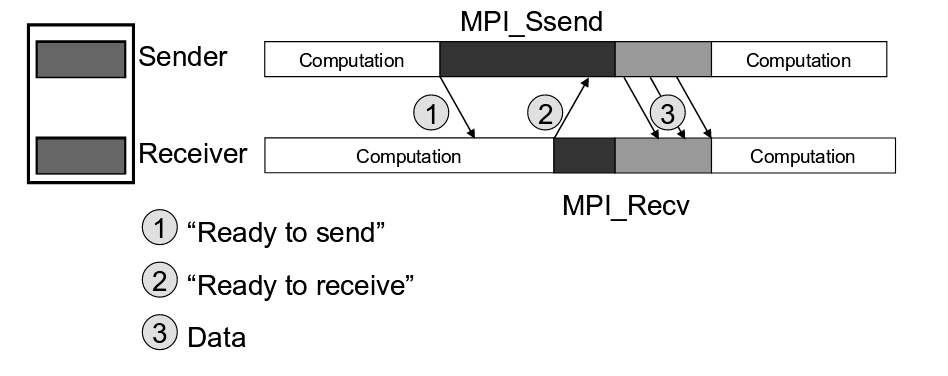
\includegraphics[width=0.9\textwidth]{img/SyncSend_gray.png}
	\subcaption{Ablauf der synchronen Sendeoperation.}
	\label{fig:sync_send}
      \end{subfigure}
      \begin{subfigure}[c]{0.45\textwidth}
	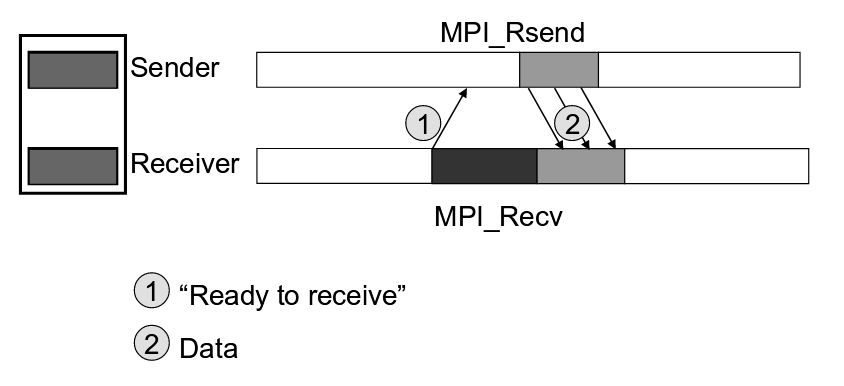
\includegraphics[width=0.9\textwidth]{img/ReadySend_gray.png}
	\subcaption{Ablauf der Ready-Send-Operation.}
	\label{fig:ready_send}
      \end{subfigure}
      \begin{subfigure}[c]{0.5\textwidth}
	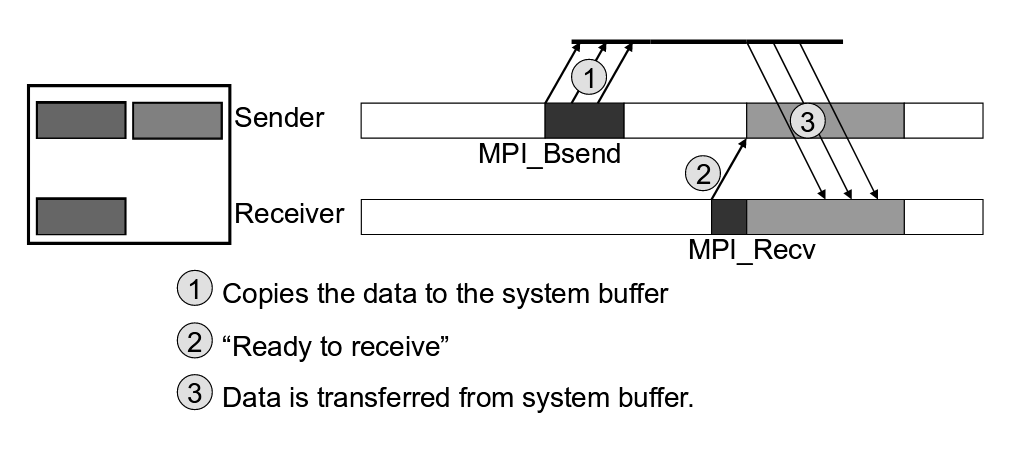
\includegraphics[width=0.9\textwidth]{img/BufferedSend_gray.png}
	\subcaption{Ablauf der gepufferten Sendeoperation.}
	\label{fig:buff_send}
      \end{subfigure}
      \caption{Ablauf unterschiedlicher Kommunikationsmodi in MPI. Quelle: \citet{mpi_p2p}}
      \label{fig:send_var}
    \end{figure}
    
    Beim synchronen Senden wird, wie in \autoref{fig:send_var}\hyperref[fig:sync_send]{.(a)} dargestellt, zunächst vom sendenden Prozess eine ``Ready to send''-Mitteilung verschickt. Auf 
    diese antwortet der empfangende Prozess mit einer ``Ready to receive''-Mitteilung. Im Anschluss findet das Senden und Empfangen der Daten statt. Durch dieses Vorgehen müssen die Prozesse
    aber gegebenenfalls auf einander warten. Die Wartezeit ist in der Abbildung durch die dunkel eingefärbten Bereiche dargestellt. Dafür wird aber nicht nur sichergestellt, dass die gesendeten
    Daten verändert werden dürfen, sondern auch, dass der Empfänger-Prozess zumindest damit begonnen hat die Daten auch zu empfangen. \citep{mpi_p2p, mpiv31}
    
    Das Ready-Send sieht wie eine einfachere synchrone Sende-Variante aus (vgl. \autoref{fig:send_var}\hyperref[fig:ready_send]{.(b)}), ist tatsächlich aber noch restriktiver. Die Methoden \code{MPI\_Rsend}
    beziehungsweise \code{MPI\_Irsend} erwarten, dass die ``Ready to receive''-Mitteilung bereits geschickt wurde, wenn sie aufgerufen werden. Nur wenn diese Mitteilung bereits eingetroffen
    ist, werden die Daten auch gesendet, ansonsten wird ein Fehler gemeldet. Diese Methode soll den System-Overhead durch Sendeoperationen und Synchronisation minimieren. Es wird jedoch 
    dazu geraten diese Methode nur zu verwenden, wenn die zeitliche Abfolge garantiert ist. \citep{mpi_p2p, mpiv31}
    
    Beim Buffered-Send werden die Daten in einem gesonderten Puffer zwischengespeichert. Dies führt durch das zusätzliche Kopieren gegebenenfalls zu weiterem Overhead, dafür kann der 
    Prozess, wie in \autoref{fig:send_var}\hyperref[fig:buff_send]{.(c)} zu erkennen, im Anschluss an den Kopiervorgang seine Arbeit fortsetzen und auch den Sendepuffer bereits verändern. 
    Die eigentliche Sendeoperation wird dann zu einem späteren Zeitpunkt nach der ``Ready to receive''-Mitteilung des Empfängers durchgeführt. Der Puffer zum Zwischenspeichern muss allerdings 
    auch durch den Nutzer zur Verfügung gestellt werden und wird nicht automatisch durch das System verwaltet. \citep{mpi_p2p, mpiv31}
    
    Bei allen blockierenden Methoden können Deadlocks auftreten. Diese können beispielsweise entstehen, wenn zwei Prozesse Daten austauschen wollen, jedoch beide mit einer Sendeoperation
    beginnen, die nicht zurückkehrt, bevor nicht auch das Empfangen der Daten begonnen wurde. Beide Prozesse werden niemals beginnen Daten zu empfangen und werden somit auch
    nie aus dem Senden zurückkehren. Abhilfe können die nicht-blockierenden Methoden liefern.
    
    Die nicht-blockierenden Methoden bestehen grundsätzlich aus zwei Aufrufen. Einer Initialisierung des Sendens/Empfangens, ohne dass auf dessen Ausführung gewartet wird, und
    einer Abschlussmethode, wie \code{MPI\_Wait}, \code{MPI\_Probe} oder \code{MPI\_Test}. Dies nicht-blockierenden Methoden ermöglicht es dem sendenden und dem empfangenden Prozess weitere Arbeiten
    auszuführen, um so möglichst Wartezeiten zu vermeiden beziehungsweise produktiv zu nutzen. Allerdings sollten weder der Sende- noch der Empfangspuffer zwischen Initialisierung und Abschluss
    verändert werden. \citep{mpi_p2p, mpiv31}
    
%     \begin{figure}[p]
%       \begin{subfigure}[c]{0.9\textwidth}
% 	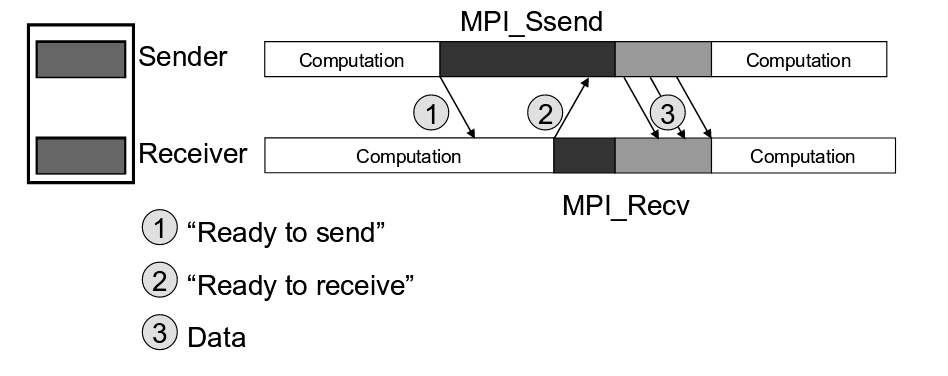
\includegraphics[width=0.9\textwidth]{img/SyncSend_gray.png}
% 	\subcaption{Ablauf der synchronen Sendeoperation.}
% 	\label{fig:sync_send}
%       \end{subfigure}
%       \begin{subfigure}[c]{0.9\textwidth}
% 	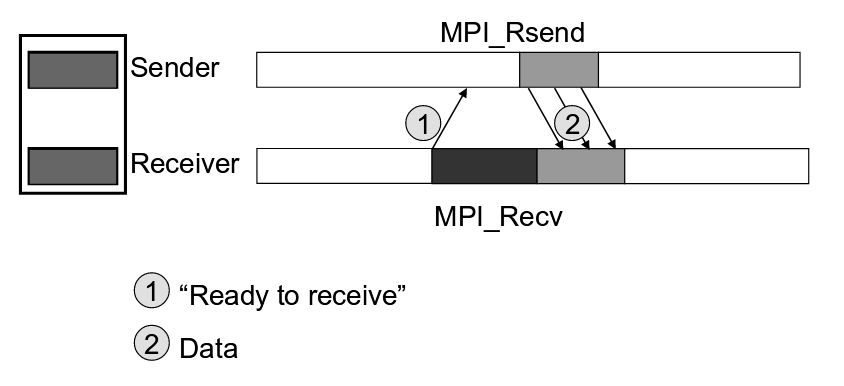
\includegraphics[width=0.9\textwidth]{img/ReadySend_gray.png}
% 	\subcaption{Ablauf der Ready-Send-Operation.}
% 	\label{fig:ready_send}
%       \end{subfigure}
%       \begin{subfigure}[c]{0.9\textwidth}
% 	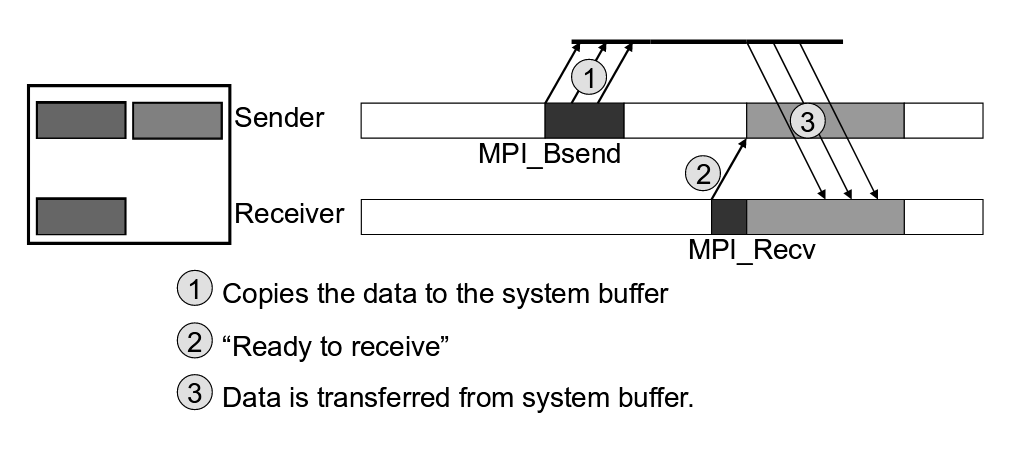
\includegraphics[width=0.9\textwidth]{img/BufferedSend_gray.png}
% 	\subcaption{Ablauf der gepufferten Sendeoperation.}
% 	\label{fig:buff_send}
%       \end{subfigure}
%       \caption{Quelle: \citet{mpi_p2p}}
%       \label{fig:send_var}
%     \end{figure}
%     \clearpage
      
    \subsection{Kollektive Kommunikation}
    \label{sec:kolkom}
    
    \begin{center}
      \begin{figure}[b]
      \centering
      \begin{subfigure}{0.9\textwidth}
      \begin{lstlisting}[language=C, label=lst:bcast, caption={Die Syntax von \code{MPI\_Bcast}}, numbers=none]
	MPI_Bcast(
	  void* data,
	  int count,
	  MPI_Datatype datatype,
	  int root,
	  MPI_Comm communicator)
      \end{lstlisting}
      \end{subfigure}
      \end{figure}
      
      \begin{figure}[b]
	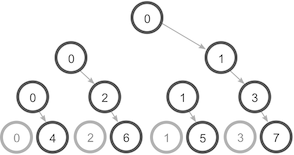
\includegraphics{img/bcast_tree_gray.png}
	\caption{Mögliche Verteilung der Daten durch \code{MPI\_Bcast}. (Quelle: \citet{mpitut})}
	\label{fig:bcast_tree}
      \end{figure}
      \end{center}
      
      Zusätzlich zur klassischen Point-to-Point-Kommuniklation bietet MPI Möglichkeiten für kollektive Kommunikation. Ein Unterschied zur direkten Kommunikation zwischen zwei Knoten ist, dass hier
      keine getrennten Send- und Receive-Operationen durchgeführt werden. Bei der kollektiven Kommunikation rufen alle Prozesse eines Kommunikators dieselbe Methode auf. Daher sind auch die Parameter
      \code{destination} und \code{tag} nicht mehr notwendig. Wie auch bei der Point-to-Point-Kommunikation gibt es bei diesen Methoden jeweils eine blockierende und eine nicht-blockierende Variante.
      
      Die einfachste kollektive Methode ist \code{MPI\_Barrier}. Diese dient nicht dem Austausch von Daten, sondern ausschließlich der  Synchronisation der Prozesse eines Kommunikators.
      Jeder Prozess, der diese Methode aufruft, wartet, bis jeder Prozess des Kommunikators diese Methode ebenfalls aufgerufen hat. Eine Deadlockgefahr besteht, falls nicht alle Prozesse
      des Kommunikators die Methode aufrufen. \citep{mpiv31}
      
      In \autoref{fig:kolkom} sind einige kollektive Methoden und ihre jeweilige Funktionsweise veranschaulicht und werden im Folgenden kurz erläutert.
      
      Der Broadcast dient dazu, Daten von einem Prozess an alle anderen zu verteilen. Die Syntax ist \autoref{lst:bcast} zu finden.

      Die meisten Parameter sind bereits aus dem vorherigen Abschnitt bekannt. Neu ist der Parameter \code{int root}. Dieser bezeichnet den Rang des Prozesses im Kommunikator,
      der die Daten an die anderen verteilen möchte. Er legt also letztlich fest welcher Prozess sendet und welcher empfängt.
      Auch wenn es auf den ersten Blick so aussehen mag, werden die Daten nicht ausschließlich vom Sender nacheinander an alle Empfänger gesendet, was linearen Aufwand
      bedeuten würde, sondern baumartig weitergegeben. In \autoref{fig:bcast_tree} wird ein möglicher Ablauf dargestellt. Durch dieses Vorgehen ist logarithmische Laufzeit erreichbar. 
      \citep{mpitut, mpiv31}
      
      \code{MPI\_Scatter} dient ebenfalls dem Verteilen von Daten von einem Prozess auf die anderen, jedoch wird hier ein Array auf alle Prozesse eines Kommunikators verteilt.
      Dies kann zum Beispiel genutzt werden, um Testdaten in einem Root-Prozess einzulesen und dann an die anderen Prozesse zu verteilen. Umgekehrt zieht \code{MPI\_Gather} die
      Daten aller Prozesse eines Kommunikators auf einem Prozess zusammen, beispielsweise um die Ergebnisse einer verteilten Berechnung auf einem Prozess zu aggregieren und
      auszugeben. Beim darunter abgebildeten \code{MPI\_Allgather} wird das Ergebnis nicht nur auf einem, sondern auf allen Prozessen gesammelt. \citep{mpitut, mpiv31}
      
      Ähnlich zu den beiden Gather-Methoden sind die Methoden \code{MPI\_Reduce} und \code{MPI\_\-Allreduce}. Auch diese sammeln Daten von allen Prozessen auf einen, respektive
      auf alle Prozesse, zusammen. Jedoch werden hierbei die Daten nicht einfach in einem Array gebündelt, sondern über den Parameter \code{MPI\_Op op} eine Operation mitgegeben,
      die auf die gesammelten Daten angewandt wird. So können aus den gesendeten Daten direkt das Maximum, Minimum, die Summe und vieles mehr bestimmt werden. \citep{mpitut, mpiv31}
      
      Zuletzt ist \code{MPI\_Alltoall} in \autoref{fig:kolkom} dargestellt. Hierbei führt quasi jeder Prozess ein Scatter durch. Man könnte es auch als \textit{Transponieren} der
      ``Prozess-Daten-Matrix'' bezeichnen. \citep{mpiv31}
      
      Von jeder dieser kollektiven Methoden gibt es wie bereits erwähnt ebenfalls eine nicht-blockierende Variante, die, der Namenskonvention folgend, durch ein eingeschobenes \code{I}
      gekennzeichnet ist. 
      
      \begin{figure}[b]
      \begin{subfigure}{0.9\textwidth}
      \begin{lstlisting}[language=C, label=lst:a2a, caption={Die Syntax von \code{MPI\_Alltoallv}}, numbers=none]
	int MPI_Alltoallv(
	  const void* sendbuffer,
	  const int sendcounts[], 
	  const int senddispls[], 
	  MPI_Datatype sendtype, 
	  void* recvbuffer, 
	  const int recvcounts[], 
	  const int recvdispls[], 
	  MPI_Datatype recvtype, 
	  MPI_Comm comm)
      \end{lstlisting}
      \end{subfigure}
      \end{figure}
      
      Außerdem gibt es für die Daten austauschenden Methoden eine \textit{vektorisierte} Variante. Alle zuvor erläuterten Methoden erwarten eine feste Anzahl an zu 
      kommunizierenden Elementen pro Prozess.
      Es kann aber vorkommen, dass zwischen unterschiedlichen Prozessen unterschiedliche Anzahlen von Elementen ausgetauscht werden müssen. Genau dies ist durch die vektorisierten Varianten, 
      zu erkennen an einem hinter dem Namen angefügten \code{v}, möglich. Diese erwarten jeweils ein Array von Anzahlen zu sendender und zu empfangender Elemente.
      Als Beispiel ist die Syntax der vektorisierten Alltoall-Methode in \autoref{lst:a2a} aufgeführt.
      
      Für $i \in \nullhaken{p-1}$ legt der $i$-te Eintrag der Arrays \code{sendcounts} und \code{recvcounts} fest, wie viele Elemente an den $i$-ten Prozess gesendet, respektive vom $i$-ten
      Prozess empfangen werden. Neu sind außerdem die \code{int}-Arrays \code{senddispls} und \code{recvdispls}. Der $i$-te Eintrag legt hier fest, ab welchem Index die Daten im 
      \code{sendbuffer} für den $i$-ten Prozess bestimmt sind, beziehungsweise ab welchem Index im \code{recvbuffer} die Daten des $i$-ten Prozesses zu empfangen sind. \citep{mpiv31}


      \begin{figure}[tbp]%
      \begin{subfigure}[l]{0.87\textwidth}
	\begin{tabular}[]{m{0.2cm} m{0.3cm}|m{0.3cm}|m{0.3cm}|m{0.3cm}|m{0.3cm}|m{0.3cm} m{1.5cm} m{0.3cm}|m{0.3cm}|m{0.3cm}|m{0.3cm}|m{0.3cm}|m{0.3cm}}
	  & \multicolumn{13}{l}{Daten $\longrightarrow$}\\
	  \cline{2-7} \cline{9-14}
	  \multirow{6}{*}{\begin{turn}{-90} Prozesse $\longrightarrow$ \end{turn}}
	  &\multicolumn{1}{|c|}{$A_0$}& & & & &\multicolumn{1}{|m{0.3cm}|}{ } &\multirow{6}{*}{\large $\xrightarrow{\text{Broadcast}}$} & \multicolumn{1}{|c|}{$A_0$}& & & & &\multicolumn{1}{|m{0.3cm}|}{ }\\
	  \cline{2-7} \cline{9-14}
	  &\multicolumn{1}{|c|}{ }& & & & &\multicolumn{1}{|c|}{ }                         & & \multicolumn{1}{|c|}{$A_0$}    & & & & &                \multicolumn{1}{|c|}{ }    \\
	  \cline{2-7} \cline{9-14}
	  &\multicolumn{1}{|c|}{ }& & & & &\multicolumn{1}{|c|}{ }                         & & \multicolumn{1}{|c|}{$A_0$}    & & & & &                \multicolumn{1}{|c|}{ }    \\
	  \cline{2-7} \cline{9-14}
	  &\multicolumn{1}{|c|}{ }& & & & &\multicolumn{1}{|c|}{ }                         & & \multicolumn{1}{|c|}{$A_0$}    & & & & &                \multicolumn{1}{|c|}{ }    \\
	  \cline{2-7} \cline{9-14}
	  &\multicolumn{1}{|c|}{ }& & & & &\multicolumn{1}{|c|}{ }                         & & \multicolumn{1}{|c|}{$A_0$}    & & & & &                \multicolumn{1}{|c|}{ }    \\
	  \cline{2-7} \cline{9-14}
	  &\multicolumn{1}{|c|}{ }& & & & &\multicolumn{1}{|c|}{ }                         & & \multicolumn{1}{|c|}{$A_0$}    & & & & &                \multicolumn{1}{|c|}{ }    \\
	  \cline{2-7} \cline{9-14}
	\end{tabular}
	\subcaption{Beim \code{MPI\_Bcast} wird ein Datensatz von einem Root-Prozess an alle anderen Prozesse gesendet und von diesen empfangen.}
      \end{subfigure}
      
      \begin{subfigure}[l]{0.87\textwidth}
	\begin{tabular}[]{m{0.2cm} m{0.3cm}|m{0.3cm}|m{0.3cm}|m{0.3cm}|m{0.3cm}|m{0.3cm} m{1.5cm} m{0.3cm}|m{0.3cm}|m{0.3cm}|m{0.3cm}|m{0.3cm}|m{0.3cm}}
	  & \multicolumn{13}{l}{Daten $\longrightarrow$}\\
	  \cline{2-7} \cline{9-14}
	  \multirow{6}{*}{\begin{turn}{-90} Prozesse $\longrightarrow$ \end{turn}}
	  &\multicolumn{1}{|c|}{$A_0$}&$A_1$&$A_2$&$A_3$&$A_4$&\multicolumn{1}{|m{0.3cm}|}{$A_5$} &\multirow{6}{*}{\large \shortstack{ $\xrightarrow{\text{ Scatter }}$ \\ $\xleftarrow[\text{ Gather }]{}$ }} & \multicolumn{1}{|c|}{$A_0$}& & & & &\multicolumn{1}{|m{0.3cm}|}{ }\\
	  \cline{2-7} \cline{9-14}
	  &\multicolumn{1}{|c|}{ }& & & & &\multicolumn{1}{|c|}{ }                         & & \multicolumn{1}{|c|}{$A_1$}    & & & & &                \multicolumn{1}{|c|}{ }    \\
	  \cline{2-7} \cline{9-14}
	  &\multicolumn{1}{|c|}{ }& & & & &\multicolumn{1}{|c|}{ }                         & & \multicolumn{1}{|c|}{$A_2$}    & & & & &                \multicolumn{1}{|c|}{ }    \\
	  \cline{2-7} \cline{9-14}
	  &\multicolumn{1}{|c|}{ }& & & & &\multicolumn{1}{|c|}{ }                         & & \multicolumn{1}{|c|}{$A_3$}    & & & & &                \multicolumn{1}{|c|}{ }    \\
	  \cline{2-7} \cline{9-14}
	  &\multicolumn{1}{|c|}{ }& & & & &\multicolumn{1}{|c|}{ }                         & & \multicolumn{1}{|c|}{$A_4$}    & & & & &                \multicolumn{1}{|c|}{ }    \\
	  \cline{2-7} \cline{9-14}
	  &\multicolumn{1}{|c|}{ }& & & & &\multicolumn{1}{|c|}{ }                         & & \multicolumn{1}{|c|}{$A_5$}    & & & & &                \multicolumn{1}{|c|}{ }    \\
	  \cline{2-7} \cline{9-14}
	\end{tabular}
	\subcaption{\code{MPI\_Scatter} verteilt ein Array von Daten auf die Prozesse. \code{MPI\_Gather} vereinigt Daten aller Prozesse in einem Array auf einem Root-Prozess.}
      \end{subfigure}
      
      \begin{subfigure}[l]{0.87\textwidth}
	\begin{tabular}[]{m{0.2cm} m{0.3cm}|m{0.3cm}|m{0.3cm}|m{0.3cm}|m{0.3cm}|m{0.3cm} m{1.5cm} m{0.3cm}|m{0.3cm}|m{0.3cm}|m{0.3cm}|m{0.3cm}|m{0.3cm}}
	  & \multicolumn{13}{l}{Daten $\longrightarrow$}\\
	  \cline{2-7} \cline{9-14}
	  \multirow{6}{*}{\begin{turn}{-90} Prozesse $\longrightarrow$ \end{turn}}
	  &\multicolumn{1}{|c|}{$A_0$}&$B_0$&$C_0$&$D_0$&$E_0$&\multicolumn{1}{|m{0.3cm}|}{$F_0$} &\multirow{6}{*}{\large $\xleftarrow{\text{Allgather}}$} & \multicolumn{1}{|c|}{$A_0$}& & & & &\multicolumn{1}{|m{0.3cm}|}{ }\\
	  \cline{2-7} \cline{9-14}
	  &\multicolumn{1}{|c|}{$A_0$}&$B_0$&$C_0$&$D_0$&$E_0$&\multicolumn{1}{|m{0.3cm}|}{$F_0$}                         & & \multicolumn{1}{|c|}{$B_0$}& & & & &\multicolumn{1}{|c|}{ }\\
	  \cline{2-7} \cline{9-14}
	  &\multicolumn{1}{|c|}{$A_0$}&$B_0$&$C_0$&$D_0$&$E_0$&\multicolumn{1}{|m{0.3cm}|}{$F_0$}                         & & \multicolumn{1}{|c|}{$C_0$}& & & & &\multicolumn{1}{|c|}{ }\\
	  \cline{2-7} \cline{9-14}
	  &\multicolumn{1}{|c|}{$A_0$}&$B_0$&$C_0$&$D_0$&$E_0$&\multicolumn{1}{|m{0.3cm}|}{$F_0$}                         & & \multicolumn{1}{|c|}{$D_0$}& & & & &\multicolumn{1}{|c|}{ }\\
	  \cline{2-7} \cline{9-14}
	  &\multicolumn{1}{|c|}{$A_0$}&$B_0$&$C_0$&$D_0$&$E_0$&\multicolumn{1}{|m{0.3cm}|}{$F_0$}                         & & \multicolumn{1}{|c|}{$E_0$}& & & & &\multicolumn{1}{|c|}{ }\\
	  \cline{2-7} \cline{9-14}
	  &\multicolumn{1}{|c|}{$A_0$}&$B_0$&$C_0$&$D_0$&$E_0$&\multicolumn{1}{|m{0.3cm}|}{$F_0$}                         & & \multicolumn{1}{|c|}{$F_0$}& & & & &\multicolumn{1}{|c|}{ }\\
	  \cline{2-7} \cline{9-14}
	\end{tabular}
	\subcaption{\code{MPI\_Allgather} vereint ebenfalls Daten aller Prozesse, allerdings erhält jeder Prozess eine Kopie des Arrays.}
      \end{subfigure}
      
      \begin{subfigure}[l]{0.87\textwidth}
	\begin{tabular}[]{m{0.2cm} m{0.3cm}|m{0.3cm}|m{0.3cm}|m{0.3cm}|m{0.3cm}|m{0.3cm} m{1.5cm} m{0.3cm}|m{0.3cm}|m{0.3cm}|m{0.3cm}|m{0.3cm}|m{0.3cm}}
	  & \multicolumn{13}{l}{Daten $\longrightarrow$}\\
	  \cline{2-7} \cline{9-14}
	  \multirow{6}{*}{\begin{turn}{-90} Prozesse $\longrightarrow$ \end{turn}}
	  &\multicolumn{1}{|c|}{$A_0$}&$A_1$&$A_2$&$A_3$&$A_4$&\multicolumn{1}{|m{0.3cm}|}{$A_5$} &\multirow{6}{*}{\large $\xrightarrow{\text{Alltoall}}$} & \multicolumn{1}{|c|}{$A_0$}&$B_0$&$C_0$&$D_0$&$E_0$&\multicolumn{1}{|m{0.3cm}|}{$F_0$}\\
	  \cline{2-7} \cline{9-14}
	  &\multicolumn{1}{|c|}{$B_0$}&$B_1$&$B_2$&$B_3$&$B_4$&\multicolumn{1}{|m{0.3cm}|}{$B_5$} & & \multicolumn{1}{|c|}{$A_1$}&$B_1$&$C_1$&$D_1$&$E_1$&\multicolumn{1}{|m{0.3cm}|}{$F_1$}\\
	  \cline{2-7} \cline{9-14}
	  &\multicolumn{1}{|c|}{$C_0$}&$C_1$&$C_2$&$C_3$&$C_4$&\multicolumn{1}{|m{0.3cm}|}{$C_5$} & & \multicolumn{1}{|c|}{$A_2$}&$B_2$&$C_2$&$D_2$&$E_2$&\multicolumn{1}{|m{0.3cm}|}{$F_2$}\\
	  \cline{2-7} \cline{9-14}
	  &\multicolumn{1}{|c|}{$D_0$}&$D_1$&$D_2$&$D_3$&$D_4$&\multicolumn{1}{|m{0.3cm}|}{$D_5$} & & \multicolumn{1}{|c|}{$A_3$}&$B_3$&$C_3$&$D_3$&$E_3$&\multicolumn{1}{|m{0.3cm}|}{$F_3$}\\
	  \cline{2-7} \cline{9-14}
	  &\multicolumn{1}{|c|}{$E_0$}&$E_1$&$E_2$&$E_3$&$E_4$&\multicolumn{1}{|m{0.3cm}|}{$E_5$} & & \multicolumn{1}{|c|}{$A_4$}&$B_4$&$C_4$&$D_4$&$E_4$&\multicolumn{1}{|m{0.3cm}|}{$F_4$}\\
	  \cline{2-7} \cline{9-14}
	  &\multicolumn{1}{|c|}{$F_0$}&$F_1$&$F_2$&$F_3$&$F_4$&\multicolumn{1}{|m{0.3cm}|}{$F_5$} & & \multicolumn{1}{|c|}{$A_5$}&$B_5$&$C_5$&$D_5$&$E_5$&\multicolumn{1}{|m{0.3cm}|}{$F_5$}\\
	  \cline{2-7} \cline{9-14}
	\end{tabular}
	\subcaption{\code{MPI\_Alltoall} ist ein simultanes MPI\_Scatter aller Prozesse. Betrachtet man die Prozesse und Daten als Matrix, wird eine Matrixtranformation durchgeführt.}
      \end{subfigure}
      
      \caption{Möglichkeiten der kollektiven Kommunikation in MPI. (Quelle: \citet{dartmouth})}%
      \label{fig:kolkom}%
\end{figure}%%      
      \clearpage
      
      

\chapter{Hauptteil}
 \label{chp:Approach1}
 
   \section{Ausgangssituation}
   \label{sec:ausgang}
    Zur Erinnerung: Wir wollen für $n \in \N_{\geq 2}$ die wechselseitigen Gravitationskräfte von $n$ Himmelskörpern berechnen. Da die größten davon die Sonnen sind und es davon bereits mehr als
    genug in unserer Galaxie gibt beschränken wir uns zunächst auf diese. Die Menge unserer $n$ Sonnen ist im Folgenden mit der Menge $\Omega$ dargestellt. Für jede Sonne
    $x \in \Omega$ muss die Gleichung
    \begin{equation}
      f_x = \sum_{\substack{y \in \Omega \\ y \neq x}} \gamma m_x  m_y \frac{y - x}{\norm{y - x}^3_2}
      \label{eq:sum_grav2}
    \end{equation}
    gelöst werden. Zunächst möchte ich die Grundstruktur des Programms vorstellen. Das Programm ist in C geschrieben und wurde in der nicht-optimierten Version von Sven 
    Christophersen zur Verfügung gestellt.
    
    Wir benötigen als ersten Schritt eine Datenstruktur, die unsere Sonnen darstellt. Diese ist in \autoref{lst:bodies} aufgeführt.
    \begin{figure}[tb]
    \centering
    \begin{subfigure}{0.9 \textwidth}
    \begin{lstlisting}[language=C, label=lst:bodies, caption={Die Struktur \code{bodies} dient der Speicherung aller mit den einzelnen Sonnen zusammenhängenden Daten}, numbers=none]
/* Struct that holds coordinates x, masses m and forces F for all particles. */
struct _bodies {
  int    *id; // id to identify each single body
  double *x;  // x-components of the masses.
  double *y;  // y-components of the masses.
  double *z;  // z-components of the masses.
  double *Fx; // x-components of the forces.
  double *Fy; // y-components of the forces.
  double *Fz; // z-components of the forces.
  double *vx; // x-components of the velocities.
  double *vy; // y-components of the velocities.
  double *vz; // z-components of the velocities.
  double *m;  // The masses.
  int     n;  // Number of masses.
  double th;  // length of one timestep.
};
typedef struct _bodies bodies;
    \end{lstlisting}
    \end{subfigure}
    \end{figure}
    In Vorbereitung einer eventuell anschließenden Vektorisierung (vgl. \todo{Ref auf Ausblick}) wurde diese Struktur als \hyperref[w:aos]{struct of arrays} (vgl. \autoref{sec:processor}) 
    angelegt.
    
    Die Komponenten der Struktur sind:
    \begin{enumerate}
     \item das Array \code{int *id}, das einer einfachen Identifizierung der Sonnen dient,
     \item die Arrays \code{double *x, *y, *z}, in denen die Position der Sonnen gespeichert werden,
     \item die Arrays \code{double *Fx, *Fy, *Fz}, in denen die Kraftvektoren, die auf die einzelnen Sonne wirken, gespeichert werden,
     \item die Arrays \code{double *vx, *vy, *vz}, in denen der Geschwindigkeitsvektor jeder Sonne gespeichert wird,
     \item das Array \code{double *m}, in dem die Massen der Sonnen gespeichert werden, und zuletzt
     \item die Werte \code{int n} und \code{double th}, die die Anzahl an Sonnen und die Länge eines Zeitschritts in Sekunden enthalten.
    \end{enumerate}
    
    Die Körper entsprechen noch keinen reellen Himmelkörpern, zu denen uns keine Daten vorliegen, sondern werden zufällig generiert. Die Sonnen werden in einem Gebiet von $\pm 1$ Lichtjahr in
    jeder Koordinatenrichtung um einen angenommenen Ursprung mit Massen zwischen einer und $15$ Sonnenmassen verteilt.\todo{echte Werte nachlesen!}

    Um nun alle gravitationellen Wechselwirkungen zu berechnen wird die Methode \code{compute_forces_bodies(...)} (vgl. \autoref{lst:compfbodies}) ausgeführt.
    Gut zu erkennen ist die matrixähnliche Struktur: Die beiden \code{for}-Schleifen entsprechen dem zeilen- und spaltenweisen durchgehen der zugehörigen $\Omega \times \Omega$-Matrix. 
    Explizit aufgestellt wird diese Matrix allerdings nicht, da dies in Bezug auf den Speicherplatz äußerst ineffizient wäre. Statt dessen wird direkt, wie in \autoref{eq:sum_grav2}
    angegeben, die kumulative Kraftwirkung für jede Sonne berechnet und in der \code{bodies}-Struktur gespeichert. Ein Teil der Kernfunktion ist in den Aufruf von \code{calc\_potential(...)}
    in Zeile 19 ausgegliedert. 
    %Der zugehörige Code ist in \autoref{lst:calcpot} zu finden. 
    Diese Methode berechnet das rein auf der Entfernung der beiden Sonnen beruhende Gravitationspotential $P(x,y)$, sodass die Formel aus \autoref{eq:sum_grav2} wie folgt dargestellt werden kann
    \[
      f_x = \sum_{\substack{y \in \Omega \\ y \neq x}} \gamma m_x  m_y P(x, y), \ \ \ \ P(x, y) := \frac{y - x}{\norm{y - x}^3_2}.
    \]
    
    Wie bereits in der Einleitung beschrieben ist das Problem mit diesem Algorithmus, dass er in Bezug auf die Laufzeit quadratisch skaliert. Läuft dieser Algorithmus mit $n = 2^{13} \approx 8.000$
    Sonnen noch in $1,097$ Sekunden durch, so braucht er bereits für $n = 2^{15} \approx 32.000$ Sonnen $17,531$ Sekunden und für $n = 2^{16} \approx 64.000$ Sonnen bereits über $70$ Sekunden.
    \footnote{Ausgeführt aufeinem Computer mit 16 Gb Arbeitsspeicher und einem Intel Core i7 mit 2,4 GHz pro Kern.} 
    Und diese Größenordnung ist weit entfernt von dem reellen Problem die Gravitationskräfte in unserer Galaxie mit etwa $100.000.000.000$ Sonnen zu berechnen.
    
    \begin{figure}[b]
    \centering
    \begin{subfigure}{0.9\textwidth}
    \begin{lstlisting}[language=C, label=lst:compfbodies,caption={Diese Methode berechnet die auftretenden Gravitationskräfte.}]
/* Computation of the resulting forces for every particle.*/
void compute_forces_bodies(bodies *b) {
  int n = b->n;
  int i, j;
  double F[3],P[3];
  double *x, *y, *z, *m;
  x = b->x;
  y = b->y;
  z = b->z;
  m = b->m;
  for (i = 0; i < n; ++i) {
    F[0] = 0.0;
    F[1] = 0.0;
    F[2] = 0.0;
    for (j = 0; j < n; ++j) {
      if (i == j) {
	continue;
      }
      calc_potential(x[i], y[i], z[i], x[j], y[j], z[j], P);
      F[0] += m[j] * P[0];
      F[1] += m[j] * P[1];
      F[2] += m[j] * P[2];
    }
    b->Fx[i] += GAMMA * m[i] * F[0];
    b->Fy[i] += GAMMA * m[i] * F[1];
    b->Fz[i] += GAMMA * m[i] * F[2];
  }
}
    \end{lstlisting}
    \end{subfigure}
    \end{figure}
    
%     \begin{subfigure}{0.9\textwidth}
%     \begin{lstlisting}[language=C, label=lst:calcpot, caption={Diese Methode berechnet für zwei Sonnen das abstandsabhängige Gravitationspotential.}]
% void calc_potential(double xi, double yi, double zi, double xj, double yj, double zj, double *P){
%   double d[3], norm, norm3;
%   d[0] = xj - xi;
%   d[1] = yj - yi;
%   d[2] = zj - zi;
%   norm = sqrt(d[0] * d[0] + d[1] * d[1] + d[2] * d[2]);
%   norm = 1.0 / norm;
%   norm3 = norm * norm * norm;
%   P[0] = d[0] * norm3;
%   P[1] = d[1] * norm3;
%   P[2] = d[2] * norm3;
% }
%     \end{lstlisting}
%     \end{subfigure}
%     \end{figure}
    
    \clearpage
    
  \section{$\mathcal{H}^2$-Matrixstruktur und Approximation}
  \label{sec:approxf}
    Nun wollen wir die in \autoref{sec:h2} vorgestellte Struktur der hierarchischen Matrizen nutzen, um den Algorithmus zu beschleunigen. Wir wollen also die Kernfunktion
    \[
     f: \Omega \times \Omega \to \R^3, \ (x,y) \mapsto \gamma m_x  m_y \frac{y - x}{\norm{y - x}^3_2}
    \]
    durch Lagrange-Interpolation der Ordnung $k$ in jeder Koordinatenrichtung auf Clustern $\tau$ und $\sigma$ des zulässigen Blocks $b = \tau \times \sigma \in \mathcal{L}^+(T_{\Omega \times \Omega})$ 
    approximieren.
    Dazu konstruieren wir Tschebyscheff-Interpolationspunkte $\xi_{\mathfrak{g}, \mathfrak{i}} \text{, } \mathfrak{g} \in \{ \tau, \sigma \}, \mathfrak{i} \in \haken{k}^3 =: M \subset \N^3$
    und erhalten so:
    \begin{eqnarray*}
      f(x,y) \approx \tilde f (x,y) 
      &=& \sum_{\nu \in M} \sum_{\mu \in M} \lag_\indt{\nu}(x) \gamma m_x m_y \frac{\xi_\inds{\mu} - \xi_\indt{\nu}}{\norm{\xi_\inds{\mu} - \xi_\indt{\nu}}^3_2} \lag_\inds{\mu}(y)\\
      &=& \gamma \sum_{\nu \in M} \lag_\indt{\nu}(x) m_x \sum_{\mu \in M} \frac{\xi_\inds{\mu} - \xi_\indt{\nu}}{\norm{\xi_\inds{\mu} - \xi_\indt{\nu}}^3_2} \lag_\inds{\mu}(y) m_y\\
      &=& \gamma \sum_{\nu \in M} \lag_\indt{\nu}(x) m_x \sum_{\mu \in M} P( \xi_\indt{\nu} , \xi_\inds{\mu} ) \lag_\inds{\mu}(y) m_y.
    \end{eqnarray*}
    Anders ausgedrückt wollen wir die Matrix $(F)_{x,y} := f(x,y)$ durch eine $\mathcal{H}^2$-Matrix $\tilde F$ approximieren. Für einen streng zulässigen Blockbaum $T_{\Omega \times \Omega}$ 
    und jeden zulässigen Block $b = \tau \times \sigma \in \mathcal{L}^+(T_{\Omega \times \Omega})$ konstruieren wir die nötigen Matrizen, mit $\mu,\nu \in M$, wie folgt:
    \begin{eqnarray*}
      E_{\tilde \tau} &:=&
	(E_{\tilde \tau})_{\mu \nu} := \lag_\indt{\nu}(\xi_{\tilde \tau, \mu}) \ \ \ \, \text{ für alle } \tilde \tau \in sons(\tau) \text{ falls } \tau \notin \mathcal{L}(T_\Omega),\\
      V_\tau &:=&
      \begin{cases}
	(V_\tau)_{x \nu}   := \lag_\indt{\nu}(x) & \ \text{ für alle } x \in \tau \text{ falls } \tau \in \mathcal{L}(T_\Omega),\\
	\sum_{\tilde \tau \in sons(\tau)} E_{\tilde \tau} V_{\tilde \tau}  & \ \text{ falls } \tau \notin \mathcal{L}(T_\Omega),\\
      \end{cases}\\
      S_b &:=& (S_b)_{\mu \nu} := P( \xi_\indt{\nu} , \xi_\inds{\mu} )\\
      E_{\tilde \sigma} &:=&
	(E_{\tilde \sigma})_{\mu \nu} := \lag_\inds{\nu}(\xi_{\tilde \sigma, \mu}) \ \ \ \, \text{ für alle } \tilde \sigma \in sons(\sigma) \text{ falls } \tau \notin \mathcal{L}(T_\Omega),\\
      W_\sigma &:=&
      \begin{cases}
	(W_\sigma)_{y \nu}   := \lag_\inds{\nu}(y) & \ \text{ für alle } y \in \sigma \text{ falls } \sigma \in \mathcal{L}(T_\Omega),\\
	\sum_{\tilde \sigma \in sons(\sigma)} E_{\tilde \sigma} W_{\tilde \sigma}  & \ \text{ falls } \sigma \notin \mathcal{L}(T_\Omega).\\
      \end{cases}      
    \end{eqnarray*}\todo{Spalten linksbündig}
    Für die unzulässigen Blöcke $b = \tau \times \sigma \in \mathcal{L}^-(T_{\Omega \times \Omega})$ müssen wir weiterhin vollbesetzte Matrizen
    \[
      N_b := (N_b)_{xy} := \gamma m_x  m_y P(x, y)
    \]
    auswerten.

    Für die Anschauung mag es helfen, sich die Faktoren $\lag_\indt{\nu} m_x =: h_x$ beziehungsweise $\lag_\inds{\mu} m_y =: h_y$ als Anteil der Masse der Sonne $x$ beziehungsweise $y$ an 
    \wlabel{\textit{Ersatzmassen}}{w:ersatzmassen} $m_{\xi_{\mathfrak{g}, \mathfrak{i}}}$ vorzustellen, wobei $\mathfrak{g} \in \{\tau, \sigma\}$ und $\mathfrak{i} \in M$ gilt.
    Durch die Interpolation werden also für weit genug entfernte Gebiete statt der echten Sonnen Ersatzkörper betrachtet, die sich an der Position der Interpolationspunkte befinden 
    und eben diese Ersatzmassen haben. 
%     Die Lagrange-Polynome gewichten also den Anteil der Masse einer Sonne an einer Ersatzmasse.
    
    \subsection{Clusterung}
    Für die oben beschriebene Approximation müssen wir einen Clusterbaum und einen streng zulässigen Blockbaum konstruieren.
    Dazu benötigen wir zunächst eine Datenstruktur für Clusterbäume. Diese finden Sie in \autoref{lst:cluster}.
    \begin{figure}[tb]
    \begin{subfigure}{0.9\textwidth}
    \begin{lstlisting}[language=C, label=lst:cluster, caption={Die Struktur \code{Cluster} vereint die Definition eines Clusters mit der eines Clusterbaumes.}, numbers=none]
struct _Cluster{
  bodies *bodies;             //related bodies
  int id;                     //id of the Cluster
  int start;                  //start index of the according subarray
  int n;                      //number of bodies in this Cluster
  double a[3];                //"upper left" corner of the bounding box
  double b[3];                //"lower right" corner of the bounding box
  double center[3];           //center of the bounding box
  double diam;                //diameter of the bounding box
  double *m;                  //substitution masses
  double *F;                  //substitution forces
  double *xs;                 //coordinates of the locations of submasses
  int num_sons;               //number of son clusters
  struct _Cluster *son[2];    //pointers to the son
};
typedef struct _Cluster Cluster;
    \end{lstlisting}
    \end{subfigure}
    \end{figure}
    
    \subsubsection{Die Datenstruktur}
    Die Datenstruktur speichert die für die Cluster notwendigen Daten sowie jeweils Zeiger auf die Sohncluster \code{Cluster *son[2]}. Jedes \code{Cluster} verweist auf die zum Baum gehörenden 
    \code{bodies *bodies}, und nutzt einen Startindex \code{int start} sowie die Anzahl \code{int n}, um auf die zum Cluster gehörigen Sonnen zu verweisen und zuzugreifen. Auch denkbar wäre es,
    nicht getrennt das \code{bodies}-Array und den Startindex zu speichern, sondern direkt auf das erste Element des zum Cluster gehörenden Teilarrays zu zeigen. Für jedes Cluster ein eigenes
    Array anzulegen würde hingegen zu Redundanz und somit unnötigem Speicherbedarf führen, da jede Ebene des Clusterbaumes eine Partition von $\Omega$ erzeugt. Die hier vorgestellte Variante
    erscheint mir am vielseitigsten ohne nennenswert unnötig Speicher zu belegen.
    
    Außerdem enthält das Cluster die, die Elemente des Clusters umschließende, bounding box (vgl. \hyperref[w:bbox]{Seite} \pageref{w:bbox}). Diese wird durch zwei Punkte in der Gestalt 
    von \code{double a[3]} und \code{double b[3]} aufgespannt. 
    Da das Zentrum mehrfach bei der Konstruktion und Teilung auftaucht ist dieses zur Laufzeitoptimierung in \code{double center[3]} abgespeichert.
    Ebenso ist der Durchmesser der bounding box in \code{double diam} hinterlegt, um ihn nur einmal bei der Konstruktion und nicht bei jeder Abfrage erneut berechnen zu müssen.
    
    Die drei Arrays \code{double *m}, \code{double *F} und \code{double *xs} repräsentieren die in den Clustern genutzten Ersatzkörper. In \code{*m} sind die \code{n} Massen, in \code{*F} 
    Ersatzkräfte und in \code{*xs} die Positionen der Ersatzkörper, beziehungsweise Interpolationspunkte $\xi_{\mathfrak{g}, \mathfrak{i}}$, gespeichert. Für jeden Interpolationspunkt muss
    eine Ersatzmasse gespeichert werden können, sodass \code{*m} $k^3$ Einträge hat.
    Da \code{*F} ein Array von dreidimensionalen Vektoren ist, enthält es $3 k^3$ Einträge. Zwar sind \code{*xs} ebenfalls dreidimensionale Punkte, jedoch bilden diese ein regelmäßiges Raster. Indem
    wir die Koordinatenprojektionen der Punkte speichern, reichen $3 k$ Einträge. Die Interpolationspunkte können dann durch 
    $\{\tcode{xs}_0, \dots ,\tcode{xs}_{k-1}\} \times \{\tcode{xs}_0, \dots ,\tcode{xs}_{k-1}\} \times \{\tcode{xs}_0, \dots ,\tcode{xs}_{k-1}\}$ rekonstruiert werden.
    Die Einträge sind jeweils nach Koordinatenrichtung zusammengefasst, also erst alle x-Koordinaten, dann die y-Koordinaten usw., um auch wieder eine ``\hyperref[w:aos]{struct of arrays}``-Struktur 
    zu bilden, um eine einfach Vektorisierung zu ermöglichen.
    
    Die Membervariable \code{int num\_sons} dient in diesem Fall der einfacheren Abfrage, ob es sich bei dem Cluster um ein Blatt oder einen inneren Knoten handelt. In allgemeineren Kontexten 
    ist es durchaus möglich, dass Cluster unterschiedlich viele Sohncluster haben. Beispielweise hat der zugehörige Blockbaum $T_{\Omega \times \Omega}$ vier Sohnblöcke pro Nicht-Blattblock. 
    
    \subsubsection{Die Konstruktion}
    \begin{figure}[t]
\begin{subfigure}{0.9\textwidth}
\begin{lstlisting}[language=C, label=lst:setup, 
		    caption={Dies sind die Kernmethoden der Konstruktion des Clusterbaumes. Die Teilung der bounding box wird hier vorgenommen
		    sowie die Sortierung der Elemente und Konstruktion der Sohncluster gestartet.}]
void _setup(Cluster *c, int depth){
[...]
  if(depth < MAX_DEPTH){		//split as long as condition is not met
    _setup_nonLeafCluster(c, depth);
  }
[...]
}
void _setup_nonLeafCluster(Cluster *c, int depth){
  int dir = _largest_direction(c);		
  int border = _sortIndices(c, dir);	//number of elements in the first son cluster
  double b1[3],a2[3];			//new bounding box points
  for(int d = 0; d < 3; d++){
    if(d == dir){
      b1[d] = c->center[d];
      a2[d] = c->center[d];
    } else {
      b1[d] = c->b[d];
      a2[d] = c->a[d];
    }
  }
  c->num_sons = 2;
  c->son[0] = _new_bound_Cluster(c->start, border, c->bodies, c->a, b1);
  _setup(c->son[0], depth+1);
  c->son[1] = _new_bound_Cluster(c->start + border, c->n - border, c->bodies, a2, c->b);
  _setup(c->son[1], depth+1);
}
\end{lstlisting}
\end{subfigure}
\end{figure}

\begin{figure}[t]
\begin{subfigure}{0.9\textwidth}
\begin{lstlisting}[language=C, label=lst:init, caption={Hier wird der Wert \code{MAX\_DEPTH} für die Abbruchbedingung berechnet.}]
void init(int argc, String* argv){
[...]
switch(argc){
  case 3:
    pot = atoi(argv[2]);
  case 2:
    INTERPOLATION_POINTS = atoi(argv[1]);
    [...]
}
  NUM_SUB_MASSES = INTERPOLATION_POINTS * INTERPOLATION_POINTS * INTERPOLATION_POINTS;
[...]
  int leaf_pot = INTERPOLATION_POINTS - 1 ? ceil(log2(2 * NUM_SUB_MASSES)) : 4;
  MAX_DEPTH = pot - leaf_pot;
[...]
}
\end{lstlisting}
\end{subfigure}
\end{figure}

\begin{figure}[t]
\begin{subfigure}{0.9\textwidth}
\begin{lstlisting}[language=C, label=lst:sort, caption={Diese Methode nimmt die Sortierung der \code{bodies} anhand einer vorgegebenen Koordinatenrichtung vor.}]
int _sortIndices(Cluster *c, int dir){
  if(0 == c->n){
    return 0;
  }
  int j, front, back;
  double *assoc_coord;
  
  //get associated coordinates of bodies
  assoc_coord = _getAssocCoord(c->bodies, dir);
  
  //sort the bodies according to clusters center
  front = 0;
  back  = c->n;
  back -= 1;
  do {
    j = c->start + front;
    
    if(assoc_coord[j] < c->center[dir]){
      front++;
    } else {
      if(assoc_coord[c->start + back] <= c->center[dir]){
	swap_bodies(c->bodies, c->start + front, c->start + back);
      }
      back--;
    }
  } while(front <= back);

  return front; //front resembles the number of elements in the left half
}
\end{lstlisting}
\end{subfigure}
\end{figure}
    Nun, da wir eine Datenstruktur für Clusterbäume definiert haben, müssen wir diesen noch erzeugen. Sei dazu eine \code{bodies} Struktur mit zufällig generierten Sonnen gegeben.
    
    Nun beginnen wir, indem wir ein Wurzelcluster mit $\tcode{id}=0$ konstruieren. Per Definition enthält es alle in \code{bodies} gegebenen Sonnen, womit die Member \code{*bodies}, \code{start} und 
    \code{n} bereits festgelegt sind. Als nächstes erzeugen wir für die gegebenen Sonnen eine bounding box mit minimalen Ausmaßen. Dazu fassen wir für jede Koordinatenrichtung die kleinsten 
    (beziehungsweise größten) Positionswerte der \code{bodies} in \code{a} (beziehungsweise \code {b}) zusammen. Alternativ könnte man, wegen der zufälligen Konstruktion der Sonnen, auch dessen 
    Grenzen als bounding box wählen. Zu dieser bounding box werden nun die Werte \mbox{\code{center[3]}} und \code{diam} berechnet. Die Member \code{double *m} und \code{double *F} bleiben mit $0$ 
    inizialisiert. Die Interpolationspunkte \code{xs} werden allerdings ebenfalls jetzt berechnet. Dazu wurden beim Start des Programmes bereits Tschebyscheff-Interpolationspunkte auf dem Intervall 
    $[-1,1]$ berechnet. Diese werden jetzt für jede Koordinatenrichtung $\iota$ auf das entsprechende Intervall $[a_\iota, b_\iota]$ des Quaders der bounding box transformiert.
    
    Um nun mit dieser Wurzel einen Clusterbaum zu konstruieren, unterteilen wir ein Cluster jeweils in Sohncluster bis eine Abbruchbedingung erfüllt ist. 
    Die wichtigsten Auszüge aus dem Code zur rekursiven Konstruktion des Clusterbaumes sind in \autoref{lst:setup}, \autoref{lst:sort} und \autoref{lst:init} aufgeführt.
    
    Da wir mit zufällig generierten und recht großen Datenmengen arbeiten, ist es nicht notwendig die Unterteilung eines Clusters in Sohncluster kardinalitätsgesteuert vorzunehmen um ein gutes load 
    balancing zu erhalten. Dies könnte bei reellen Daten möglicherweise notwendig werden, wenn es in der betrachteten Menge $\Omega$ große Bereiche mit sehr wenigen Körpern gibt. 
    Der hier vorgestellte Algorithmus unterteilt die Cluster auf jeder Stufe des Baumes rein geometrisch durch eine Mittelebene. Dazu wird zunächst die Richtung der größten Ausdehnung der bounding
    box bestimmt und dann in dieser Koordinatenrichtung mittig unterteilt. Während dieser Unterteilung werden die zunächst ungeordneten \code{bodies} gemäß ihrer Zugehörigkeit zu einem der beiden
    Sohncluster sukzessive sortiert.
    
    Die Methode \code{\_sortIndices} beruht, über die gesamte Konstruktion des Clusterbaumes betrachtet, auf der Grundidee von Quicksort. Für die größte Richtung $[a_\iota, b_\iota]$
    des Quaders, der die bounding box darstellt, wird als Quasi-Pivotelement jeweils die Mitte $c_\iota = \frac{a_\iota + b_\iota}{2}$ dieser Richtung gesetzt und die Sonnen entsprechend ihrer 
    Position in die linke oder rechte Hälfte einsortiert. Anders als bei Quicksort wird auf Grund der gewählten Abbruchbedingung die Liste nicht vollständig sortiert. Für den Algorithmus ist
    die Zugehörigkeit der Sonnen zu bestimmten Clustern die entscheidende Information.
    
    Nach \hyperref[def:clusterbaum]{Definition}\autoref{def:clusterbaum} wurden zwei Beispiele für Abbruchbedingungen erwähnt. Wegen der zufälligen Generierung lässt sich die ungefähre Anzahl Elemente
    in den Blattclustern anhand der Tiefe des Baumes schätzen. Indem wir als Abbruchbedingung eine maximale Tiefe für den Clusterbaum festlegen, stellen wir gleichzeitig sicher, dass der Clusterbaum
    ein vollständiger Binärbaum wird.
    Der Wert \code{MAX\_DEPTH} für die Abbruchbedingung wird gleich zu Beginn des Programmlaufs auf Basis der Anzahl an Sonnen ($|\Omega| = 2^{\tcode{pot}}$), und der Interpolationsordnung $k$ 
    berechnet. Dabei gilt:
    \begin{equation*}
      \tcode{MAX\_DEPTH} := \tcode{pot} - \mathfrak{l}, \ \ \ \ \ \ \ \ \ \ \ \ 
      \mathfrak{l} :=
      \begin{cases}
	\lceil \log_2(2 k^3) \rceil & \text{falls } k > 1\\
	4			    & \text{falls } k = 1
      \end{cases}
    \end{equation*}
    Bei einer Baumtiefe von \code{pot} wären die Blattcluster um Schnitt gerade einelementig. Indem die Abbruchbedingung die Tiefe des Clusterbaumes auf $\tcode{pot} - \mathfrak{l}$ begrenzt,
    enthalten die Blattknoten im Schnitt gerade $2^\mathfrak{l}$ Elemente.
    Durch diese Baumtiefenreglierung wird für $k > 1$ die nächsthöhere Zweierpotenz zur doppelten Anzahl an Interpolationspunkten als durchschnittliche Anzahl Sonnen pro Blattcluster festgelegt. 
    Für die Interpolationsordnung $k = 1$ wäre dies eine zu feine Zerlegung. Daher wird hier $\mathfrak{l}$  auf den Wert $4$ und damit die durchschnittliche Blattgröße auf $2^4 = 8$ gesetzt.
    Indem die Blattgröße im Schnitt auf ungefähr das Doppelte der Anzahl an Interpolationspunkten festgelegt wird, soll eine gute Balance zwischen Genauigkeit und Laufzeit erreicht werden.
        
    Für die Blattcluster ist keine eigne setup-Methode notwendig, da der Konstruktor \mbox{\code{\_new\_bound\_Cluster(...)}} zunächst alle Werte für ein Blattcluster setzt. Die Methode \linebreak
    \mbox{\code{\_setup(...)}} entscheidet also anhand der Stufe ob ein Cluster ein Blattcluster bleibt, oder durch Unterteilung zu einem Nicht-Blattcluster wird.

    \subsection{Vorwärtstransformation}
    \begin{figure}[t]
  \begin{subfigure}{0.9\textwidth}
    \begin{lstlisting}[language=C, label=lst:forw, caption={Diese Methode dient dem rekursiven Aufruf der Vorwärtstransformation und delegiert die Konstruktion der Ersatzmassen.
							    Dabei wird zwischen Blatt-und Nicht-Blattclustern unterschieden.}]
void forward(Cluster *c){
  if(c->num_sons){
      _forward_nonLeaf(c);
  } else {
      _forward_leaf(c);
  }
}
    \end{lstlisting}
  \end{subfigure}
\end{figure}

\begin{figure}[p]
  \begin{subfigure}{0.9\textwidth}
    \begin{lstlisting}[language=C, label=lst:forwnonleaf, caption={Diese Methode arbeitet auf den Transfermatrizen und ruft daher zuerst rekursiv die Vorwärtstransformation für die Sohncluster auf.}]
void _forward_nonLeaf(Cluster *c){
  int i, j, k, w, wj, son, ison, json, kson, wson, wsonj;
  double sum, l1, l2, l3;

  forward(c->son[0]);	//recursiv call for first son
  forward(c->son[1]);	//recursiv call for second son

  //for all submasses
  for(i = 0; i < INTERPOLATION_POINTS; i++){
    for(j = 0; j < INTERPOLATION_POINTS; j++){
      wj = i * INTERPOLATION_POINTS + j;
      for(k = 0; k < INTERPOLATION_POINTS; k++){
	w = wj * INTERPOLATION_POINTS + k;
	sum = 0.0;
	
	//for all sons
	for(son = 0; son < 2; son++){
	  //for all sons submasses
	  for(ison = 0; ison < INTERPOLATION_POINTS; ison++){
	    l1 = lagrange(c, i, 0, c->son[son]->xs[ison]);
	    for(json = 0; json < INTERPOLATION_POINTS; json++){
	      wsonj = ison * INTERPOLATION_POINTS + json;
	      l2 = l1 * lagrange(c, j, 1, c->son[son]->xs[INTERPOLATION_POINTS + json]);
	      for(kson = 0; kson < INTERPOLATION_POINTS; kson++){
		wson = wsonj * INTERPOLATION_POINTS + kson;
		l3 = l2 * lagrange(c, k, 2, c->son[son]->xs[2 * INTERPOLATION_POINTS + kson]);

		//calculate the substitution mass
		sum += c->son[son]->m[wson] * l3;
	      }
	    }
	  }
	}
	c->m[w] = sum;
      }
    }
  }
}     
    \end{lstlisting}
  \end{subfigure}
\end{figure}

\begin{figure}[p]
  \begin{subfigure}{0.9\textwidth}
    \begin{lstlisting}[language=C, label=lst:forwleaf, caption={Diese Methode erstellt die Clusterbasis des Clusterbaumes.}]
void _forward_leaf(Cluster *c){
  if(0 == c->n){ return; }
  int i, j, k, l, m, w, wj;
  double x, y, z, *mass, l1, l2, l3;
  bodies *b = c->bodies;
  mass = b->m;

  for(i = 0; i < NUM_SUB_MASSES; i++){
    c->m[i] = 0.0;
  }

  //for all linked actual masses
  for(l = 0; l < c->n; l++){
    m = c->start + l;
    x = b->x[m];
    y = b->y[m];
    z = b->z[m];

    //for all interpolation points:
    for(i = 0; i < INTERPOLATION_POINTS; i++){
      l1 = lagrange(c, i, 0, x);
      for(j = 0; j < INTERPOLATION_POINTS; j++){
	wj = i * INTERPOLATION_POINTS + j;
	l2 = l1 * lagrange(c, j, 1, y);
	for(k = 0; k < INTERPOLATION_POINTS; k++){
	  //actual interpolation point:
	  w = wj * INTERPOLATION_POINTS + k;
	  //actual lagrange weight:
	  l3 = l2 * lagrange(c, k, 2, z);

	  //calculate the substitution mass
	  c->m[w] += mass[m] * l3;
	}
      }
    }
  }
}   
    \end{lstlisting}
  \end{subfigure}
\end{figure}
    Nun können wir uns an die Berechnung der Gravitation machen.
    Um eine Matrix-Vektor-Multiplikation mit der Matrix $\tilde F$ auf zulässigen Blöcken auszuwerten, muss diese Operation als erstes auf den Matrizen $W_\sigma$ ausgewertet werden.
    Die Auswertung der Matrizen $W_\sigma$ nennt man auch \textit{Vorwärtstransformation}.
    
    Da wir die Gravitationskräfte für alle Sonnen in $\Omega$ berechnen wollen, ist es sinnvoll die Vorwärtstransformation einfach für alle $\sigma \in T_\Omega$ durchzuführen. Dies geschieht
    im vorliegenden Programm durch einen Aufruf von \code{forward(Cluster *c)} mit $root(T_\Omega)$.
    Die Methode \code{forward(...)} unterscheidet zwischen Blatt- und Nicht-Blattclustern, und ruft entsprechend die Methode \code{\_forward\_Leaf(Cluster *c)} oder \code{\_forward\_nonLeaf(Cluster *c)}
    auf. Die Methode \code{\_forward\_Leaf(...)} entspricht der Konstruktion und Auswertung der Matrizen $W_\sigma$ anhand der Sonnen $x \in \sigma$, die Methode \code{\_forward\_nonLeaf(Cluster *c)} 
    der anhand der Sohncluster.
    Für letztere müssen daher die Ergebnisse der Söhne bereits vorliegen. Daher ruft diese als ersten Schritt \code{forward(cs)} für alle Sohncluster \code{cs} auf. Auf diese Weise durchlaufen die 
    Methoden gemeinsam betrachtet den Clusterbaum rekursiv. Der Code der drei Methoden ist in \autoref{lst:forw}, \autoref{lst:forwnonleaf} und \autoref{lst:forwleaf} zu finden.
    
    Durch die Methode \code{\_forward\_Leaf(Cluster *c)} werden, wie auf \hyperref[w:ersatzmassen]{Seite} \pageref{w:ersatzmassen} beschrieben, für alle Interpolationspunkte 
    $\xi_{\tcode{c}\mu} \in \bigtimes_{i=0}^2 \{\tcode{xs}_{i \cdot k}, \dots ,\tcode{xs}_{(i+1) \cdot k-1}\}, \mu \in M$ durch
    \[
      \tcode{m}_{\xi_{\tcode{c}\mu}} = \tcode{m}_\mu := \sum_{y \in \tcode{c}} \lag_{\tcode{c},\mu}(y) m_y
    \]
    die Ersatzmassen in der Clusterbasis berechnet und gespeichert. Die Methode \code{\_forward\_nonLeaf(Cluster *c)} berechnet ebenfalls Ersatzmassen, jedoch nicht aus allen Sonnen des Clusters,
    sondern aus den Interpolationspunkten und Ersatzmassen der Sohncluster (vgl. \autoref{sec:transmat}).
    
    Stellt man sich den Baum von der Wurzel aus nach unten hängend vor, werden also die Massen der Sonnen in den Baum hochgezogen. Je höher die Stufe des Baumes, um so gröber ist die Approximation.
    
    
    \subsection{Auswertung der Kopplungsmatrizen}
    Der nächste Schritt in der Auswertung ist die Multiplikation mit den Kopplungsmatrizen $S_b$. Da diese Matrizen, im Gegensatz zu den Clusterbasen $V_\tau$ und $W_\sigma$, vom Block und damit
    von beiden und nicht nur von einem Cluster abhängen, müssen wir nun den Blockbaum $T_{\Omega \times \Omega}$ durchlaufen. 
    Gleichzeitig können wir in diesem Schritt die Nahfeldmatrizen $N_b$, die ebenfalls von den Blöcken abhängen, auswerten. 
    
    Den Blockbaum haben wir nicht explizit aufgestellt. Das ist auch nicht notwendig, da wir ihn implizit konstruieren können und somit keinen Speicherplatz benötigen.
    Wir durchlaufen unseren impliziten Blockbaum, indem wir, beginnend mit dem Wurzelblock $b_{root} = root(T_\Omega) \times root(T_\Omega)$, für jeden Block $b = \tau \times \sigma$ prüfen, ob
    \begin{enumerate}
      \item $\mathcal{Z}_\eta(\tau,\sigma) = \ttit{zulässig}$ erfüllt ist. Ist dies der Fall haben wir, unabhängig davon, ob $\tau \in \mathcal{L}(T_\Omega)$ oder 
      $\sigma \in \mathcal{L}(T_\Omega)$ gilt, einen Blattblock erreicht und können $S_b$ auswerten. 
      \item Ist $\mathcal{Z}_\eta(\tau,\sigma) = \ttit{unzulässig}$, prüfen wir, ob 
      \begin{enumerate}
	\item $\tau, \sigma \in \mathcal{L}(T_\Omega)$. Falls $\tau$ und $\sigma$ Blattcluster sind, haben wir ebenfalls einen Blattblock erreicht, können aber nicht approximieren und müssen
	daher $N_b$ auswerten.
	\item Sind $\tau$ und $\sigma$ aber keine Blattcluster, so können wir durch folgende Zuweisung rekursiv fortfahren:	
      \end{enumerate}
    \end{enumerate}
    Für $\tilde \tau_0 \neq \tilde \tau_1 \in sons(\tau)$ und $\tilde \sigma_0 \neq \tilde \sigma_1 \in sons(\sigma)$ definieren wir Sohnblöcke
    \begin{eqnarray*}
      \tilde b_0 := \tilde \tau_0 \times \tilde \sigma_0 & \ \ \ \ \ \ \ \ \ \ \ \ & \tilde b_1 := \tilde \tau_0 \times \tilde \sigma_1\\
      \tilde b_2 := \tilde \tau_1 \times \tilde \sigma_0 & \ \ \ \ \ \ \ \ \ \ \ \ & \tilde b_3 := \tilde \tau_1 \times \tilde \sigma_1.
    \end{eqnarray*}
    
    Durch dieses Vorgehen konstruieren wir implizit einen streng zulässigen Blockbaum. Zulässige Blöcke werden automatisch Blattblöcke, da die Rekursion dort nicht fortgesetzt wird.
    Außerdem werden die Sohnblöcke immer aus genau einer Stufe des Clusterbaumes gebildet, bei welchem wir sichergestellt haben, dass er als vollständiger Binärbaum konstruiert wird. 
    Daher ist auch sichergestellt, dass unzulässige Blattblöcke nur aus Blättern des Clusterbaumes bestehen können.
    
    \begin{figure}[tb]
    \begin{subfigure}{0.9\textwidth}
    \begin{lstlisting}[label=lst:eval, caption={Durch diese rekursive Struktur wird ein impliziter Blockbaum durchlaufen, um die Matrizen $S_b$ bzw. $N_b$ auszuwerten.}]
void _eval(Cluster *ct, Cluster *cs){
  if(admissable(ct, cs)){
      _eval_CC(ct, cs);
  } else {
    if (ct->num_sons && cs->num_sons){	//both clusters have sons left:
      _eval(ct->son[0], cs->son[0]);
      _eval(ct->son[0], cs->son[1]);
      _eval(ct->son[1], cs->son[0]);
      _eval(ct->son[1], cs->son[1]);
    } else {                          	//no son clusters left but still not admissable:
      _eval_full(ct, cs);
    }
  }
  // world.rank?:current_level?:printf("\nfirst admissable block on level %d\n", first_admissable);
  // world.rank?:current_level?:printf("split depth: %d\n", SPLIT_DEPTH);
}
    \end{lstlisting}
    \end{subfigure}
    \end{figure}
    
    Für jeden Blattblock $b = \tau \times \sigma$ wird also
    \begin{enumerate}
     \item für alle $x \in \tau$ und $y \in \sigma$ die Funktion $f$ ausgewertet und direkt in den \code{bodies} gespeichert, falls $b$ unzulässig ist, oder
     \item für alle Interpolationspunkte $\xi_\indt{\nu} \text{, } \xi_\indt{\nu}$, mit $\nu,\mu \in M$ der Ausdruck $P(\xi_\indt{\nu} , \xi_\indt{\nu})$ ausgewertet und mit den in der 
     Vorwärtstransformation berechneten Ersatzmassen $\tcode{m}_\mu$ multipliziert, falls $b$ zulässig ist.
    \end{enumerate}
    
    Anschaulich werden in diesem Schritt in den zulässigen Blöcken aus den Ersatzmassen und Interpolationspunkten Quasi-Ersatzkräfte\footnote{An dieser Stelle wird nur die 
    Masse des Source-Clusters $\sigma$ verrechnet. Daher handelt es sich im physikalischen Sinne noch nicht um eine Kraft.} berechnet. 

    \subsection{Rückwärtstransformation}
    Der letzte Schritt der Berechnung ist die Auswertung der Matrizen $V_\tau$. Diesen Schritt nennt man auch \textit{Rückwärtstranformation}.
    
    Auch dieser Schritt hängt wieder ausschließlich von den Clustern ab. Daher kann die Rückwärtstranformation wieder unabhängig von den Blöcken für den gesamten Clusterbaum $T_\Omega$ ausgeführt
    werden. Wir rufen dazu, wieder mit $root(T_\Omega)$ , die Methode \code{backward(Cluster *c)} auf. Wie bereits bei der Vorwärtstransformation unterscheidet diese Methode, ob es sich bei
    dem aktuellen Cluster um ein Blatt- oder ein Nicht-Blattcluster handelt und delegiert die Arbeit entsprechend an die Methoden \code{\_backward\_Leaf(Cluster *c)} und 
    \code{\_backward\_nonLeaf(Cluster *c)}. Anders als bei der Vorwärtstransformation müssen bei der Rückwärtstransformation die Ergebnisse des Vaterclusters für die Söhne vorliegen. Daher gibt die
    Methode \code{_backward_nonLeaf(Cluster *c)} die approximierten Quasi-Kräfte, gewichtet über die Lagrange-Polynome, an die Sohncluster weiter. Für alle Söhne $\tilde{\tcode{c}} \in sons(\tcode c)$
    und alle $\mu \in M$ wird
    \[
      \tcode{F}_{\tcode{c},\tilde{\tcode{c}},\mu} = \sum_{\nu \in M} \lag_{\tcode{c},\nu}(\xi_{\tilde{\tcode{c}},\mu} \tcode{F}_{\tcode{c},\nu}
    \]
    zu den dort eventuell bereits aus der Auswertung der Kopplungsmatrizen vorhandenen Quasi-Ersatzkräfte addiert.
    
    Schließlich werden in der Methode \code{_backward_Leaf(Cluser *c)} die Quasi-Ersatzkräfte $\tcode{F}_{\tcode{c},\nu}$, $\nu \in M$, über die Lagrange-Polynome gewichtet auf alle Sonnen 
    $x \in \tcode{c}$ verteilt und mit deren Masse $m_x$ multipliziert. Da auch hier bereits aus der Nahfeldauswertung Kräfte vorhanden sind, müssen diese approximierten Kräfte\footnote{Durch die
    Multiplikation mit $m_x$ werden die Quasi-Kräfte im physikalischen Sinne zu Kräften vervollständigt.} zu den vorhandenen addiert werden.
    
    \TODO{Da diese Methoden analog zu denjenigen der Vorwärtstransformation funktionieren sind diese hier nicht (oder nur im Anhang) aufgeführt.} 

  \clearpage
 
 \section{Parallelisierung}
\label{sec:parallelpart}
  Im vorherigen Kapitel haben wir die Berechnung der Gravitationskräfte durch Interpolation approximiert. Dadurch konnten wir die Technik \hquad nutzen um den Rechenaufwand des Algorithmus zu 
  beschleunigen.
  Um die absolute Laufzeit aber noch weiter zu reduzieren sind wir an einer parallel arbeitende Variante dieses Algorithmus interessiert. In diesem Kapitel wird ein Ansatz vorgestellt.
  
  Ziel ist es, zunächst einen einfachen Algorithmus zu entwerfen. Daher beschränken wir uns auf Parallelisierung nach dem Message-Passing-Modell unter Verwendung von MPI. Wir können also 
  $p \in \N$ Prozesse starten. Jeder von diesen hat eine eindeutige $id \in \nullhaken{p-1}$ und seinen privaten Speicherbereich. Insbesondere ist in diesem Modell Shared-Memory ausgeschlossen. 
  Außerdem können die Prozesse miteinander kommunizieren um Daten auszutauschen. Die Menge der Prozesse wird im Folgen mit $\Proc$ bezeichnet.

  
  \subsection{Arbeitsverteilung}
  \label{sec:work}
    Damit wir von parallel arbeitenden Prozessen profitieren können, muss die Arbeit möglichst gleichmäßig auf diese Prozesse verteilt werden. Wir folgen, in modifizierter Variante, dem von 
    \citet{distrh2} vorgestellten Cluster-zentrierten Ansatz. 
    Dieser basiert auf dem Grundgedanken, dass für Vorwärts- und Rückwärtstranformation ausschließlich Daten zwischen Vater- und Sohnclustern ausgetauscht werden müssen. Daher ist es besonders 
    effektiv, wenn möglichst viele Söhne durch den selben Prozess verarbeitet werden, wie der Vater. Besonders einfach wird das Verteilen der Cluster und das Loadbalancing, wenn wir $p$ als 
    Zweierpotenz $p = 2^q$ wählen. Da dann die Anzahl von Clustern in $T_\Omega^{(q)}$ gerade $p$ entspricht, können wir diese Ebene, zuzüglich der Sohncluster, optimal auf die Prozesse verteilen.
    Wir gehen im Folgenden immer von einer so gewählten Anzahl Prozesse aus.
    
    Um diesen Ansatz auf den Algorithmus zu übertragen, wird in der in \autoref{lst:init} aufgeführten init-Methode die globale Variable $\tcode{SPLIT_DEPTH} = log_2(p)$ gesetzt. 
    Außerdem bekommt die Datenstruktur \code Cluster einen weiteren Member: \code{int activ}. In diesem  wird die $id$ des für dieses Cluster zuständigen Prozesses gespeichert.
    
    Zudem gibt es aber noch Cluster auf den Ebenen $T_\Omega^{<q} := T_\Omega^{(0)},\dots,T_\Omega^{(q-1)}$. Um ein Cluster $C \in T_\Omega^{<q}$ zu klassifizieren nutzt jeder Prozess $P \in \Proc$
    mit $id_P$ zwei Konstanten. Gilt für alle Nachfahren $\tilde C \in sons*(C)$ $C->activ \neq id_P$  , wird der Member \code {C->activ} auf die \code{int}-Konstante \code inactiv gesetzt. Gibt es aber Nachfahren,
    für die 
    der Prozess selbst zuständig ist, so wird 
    
  
  \subsection{Datenverteilung}
  \label{sec:data}
    \TODO{Eine der ersten und grundlegenden Fragen, die bei parallel arbeitenden Programmen geklärt werden muss, ist, wo welche Daten vorhanden sind. Ein Möglicher Ansatz wäre, dass jeder Prozess
    eine Kopie aller Daten hat.}

% \chapter{Ansatz Teil 2}\label{chp:Approach2}
%   \section{Ansatz Teil 2 Unterkapitel 1}
%     \blindtext
%   \section{Ansatz Teil 2 Unterkapitel 2}
%     \blindtext
%   \section{Ansatz Teil 2 Unterkapitel n}
%     \blindtext

\chapter{Evaluation}
\label{chp:eval}
  \citet{distrh2} haben gezeigt, dass deren paralleler Ansatz sehr nah an die optimale parallele Effizienz von $\mathcal{O}(\frac{nk}{p})$ herankommt, falls $n$ deutlich größer als $p$ ist.
  Dabei gilt: $n := |\Omega|$ ist die Anzahl Sonnen, $p := |\Proc|$ ist die Anzahl Prozesse und $k := k_0^3$ ist die Anzahl Interpolationspunkte, mit dem Grad der eindimensionalen Lagrange-Polynome 
  $k_0$. Außerdem sei im Folgenden $m := \frac{n}{p}$ die durchschnittliche Anzahl Elemente pro Prozess.
  
  Im Folgenden gilt es, die Argumentation von \citet{distrh2} auf den vorliegenden Algorithmus zu übertragen und durch Daten aus praktischen Laufzeitmessungen zu stützen. Da unser Algorithmus 
  mit impliziten Blockbäumen und \hquad arbeitet, wird die Konstruktion nicht weiter behandelt. Stattdessen konzentrieren wir uns auf eine Abschätzung für die Laufzeit.
  
  \section{Theoretische Abschätzung}
  \label{sec:theo}
  
  Zunächst treffen wir auch für diesen Abschnitt eine Annahme, die wir bereits bei der Vorstellung des Algorithmus als sinnvoll erachteten:
  \begin{ann} \ \\
  \label{ann:nodes}
    Es existiert $q \in \N$, sodass für $p := \left| \Proc \right|$ gilt:
    \[ p = 2^q. \]
  \end{ann}
  
  Zusätzlich zu der sichergestellten vollständigen Binärbaumstruktur benötigt der Clusterbaum für einige Abschätzungen weitere Eigenschaften:
  
  \begin{ann} \ \\
  \label{ann:tree}
    Es existiert eine Konstante $C_{st}$, sodass für alle Teilbäume $T_{sub}$ mit $\tau := root(T_{sub}) \in T_\Omega^{(q)}$ gilt:
    \[
     |T_{sub}|\footnotemark \leq C_{st} \frac{n}{kp} \ \ \text{ und } \ \ |\tau| \leq C_{st}\frac{n}{p}.
    \]
  \end{ann}
  \footnotetext{$|T_{sub}|$ bezeichnet die Anzahl Knoten im Baum.}
  
  Diese Annahme wurde durch die Wahl der Abbruchbedingung bei der Konstruktion des Clusterbaumes sichergestellt. Es gilt $|T_{sub}| = \frac{1}{2} \frac{n}{kp}$ (vgl. \autoref{eq:l}),
  da jeder Prozess gerade einen Teilbaum konstruiert, wie er zuvor vom gesamten nicht-parallelisierten Algorithmus vorgenommen wurde (vgl. letzter Absatz in \autoref{sec:data}). Zwar lässt sich die
  Anzahl Elemente der Cluster $\tau \in T_\Omega^{(q)}$ nicht exakt angeben, da die Unterteilung in Sohncluster nicht nach Kardinalität vorgenommen wird, jedoch beträgt diese im Schnitt gerade 
  $m = \frac{n}{p}$. Die Konstante $C_{st}$ kann also als $\approx 1$ angenommen werden.
  
  Die Methode \code{_setup(Cluster *c, int depth)}, die in unserem Algorithmus die Verteilung der Cluster auf Prozesse vornimmt, gewährleistet einige Eigenschaften, die wir im Folgenden noch benötigen
  werden.
  
  \begin{bem}
    (Zuständigkeiten)\\
    Für den verteilten Clusterbaum $T_\Omega$ gelten folgende Eigenschaften:
    \begin{equation}
      \text{Für } \tau \in T_\Omega^{(\geq q)} \text{ existiert genau ein } P \in \Proc \text{ mit } \tau.\tcode{activ} = id_P.
    \end{equation}
    \begin{equation}
      \text{Jeder Prozess } P \in \Proc \text{ berechnet auf jeder Ebene } T_\Omega^{(q')}, \ q' \in \nullhaken{q-1} \text{ genau eine Transfermatrix.}\label{eq:log}
    \end{equation}\newline
    Aus \autoref{eq:log} folgt direkt mit $q = \log_2 p$ (vgl. \autoref{sec:work}):
    \begin{equation}
      \text{Die Anzahl Transfermatrizen } E_\tau, \ \tau \in T_\Omega^{(\leq q)} \text{ pro Prozess beträgt } q.\tag{\ref{eq:log}'}
    \end{equation}
  \end{bem}

  Da wir einen parallel arbeitenden Algorithmus haben, ist es für die Abschätzung des Rechenaufwandes nicht ausreichend, die Anzahl an Operationen zu zählen. Da die Prozesse kommunizieren müssen, ist 
  regelmäßig eine Synchronisation der Prozesse notwendig. So wird es vorkommen, dass ein Prozess $P_i$ schneller seine Berechnungen durchführt als ein Prozess $P_j$ und dann auf diesen warten muss,
  bevor die Kommunikation stattfinden kann. 
  
  Daher verwenden wir einen ähnlichen Ansatz, wie er auch beim BSP-Modell \citep{bsp} verwendet wurde: Die gesamte Berechnung wird in eine Sequenz von $s \in \N_0$ \textit{Superschritten} eingeteilt,
  die jeweils unabhängig von den anderen Prozessen von einem Prozess durchgeführt werden können. Der $i$-te Superschritt startet simultan, sobald alle Prozesse den $(i-1)$-ten Superschritt abgeschlossen
  haben, $i \in \haken{s}$. Als Zeiteinheit verwenden wir die abstrahierte Einheit \textit{Zyklus}. Ein Zyklus sei dabei lang genug, um eine arithmetische Operation, einen Speicherzugriff oder eine 
  Sende- oder Empfangsoperation für einen \code{double}-Wert durchzuführen.
  
  \begin{lem}
  \label{lem:vorw}
    (Vorwärtstransformation)\\
    Die parallele Vorwärtstransformation benötigt $\mathcal{O}(\frac{nk}{p}+k^2 \log_2p)$ Zyklen.
  \end{lem}
  
  \textit{Beweis:} 
  Die gesamte Vorwärtstransformation kann in einem Superschritt abgehandelt werden, da keinerlei Kommunikation notwendig ist. 
  
  Zunächst werden alle aktiven Cluster ausgewertet. Seien also $P \in \Proc$ und $T_\Omega^P$ der aktive Teilbaum dieses Prozesses. Für ein Blattcluster $\sigma \in \mathcal{L}(T_\Omega^P)$ müssen 
  für alle $k$ Ersatzmassen $|\sigma|$ Berechnungen durchgeführt werden.  
  Dann gilt  mit \hyperref[ann:tree]{Annahme }\ref{ann:tree}, dass insgesamt
  \begin{align*}
    \sum_{\sigma \in \mathcal{L}(T_\Omega^P)} k|\sigma| &= k\sum_{\sigma \in \mathcal{L}(T_\Omega^P)} |\sigma| \approx k m\\
    &\leq C_{st}\frac{nk}{p}
  \end{align*}
  Operationen ausgeführt werden müssen.
  
  Für Nicht-Blattcluster $\sigma \in T_\Omega^P \backslash \mathcal{L}(T_\Omega^P)$ sind für die $k$ Ersatzmassen und beide Sohncluster wiederum $k$ Auswertungen notwendig. Damit folgt, dass weitere
  \begin{align*}
    &\sum_{\sigma \in T_\Omega^P \backslash \mathcal{L}(T_\Omega^P)} \ \ \sum_{\tilde \sigma \in sons(\sigma)} 2k^2 \leq \sum_{\tilde \sigma \in T_\Omega^P} 2k^2\\
    &= 2k^2 |T_\Omega^P| \leq 2k^2 C_{st} \frac{n}{kp} = 2C_{st}\frac{nk}{p}
  \end{align*}
  Operationen ausgeführt werden müssen.
  
  Für die Ebenen $T_\Omega^{(<q)}$ werden nun jeweils die $k$ Ersatzmassen aus den $k$ Ersatzmassen eines Sohnclusters berechnet. Da es gerade $q = \log_2(p)$ Ebenen gibt, führt dies insgesamt zu obiger
  Abschätzung. \qed
  
  \begin{lem}
  \label{lem:ruckw}
    (Rückwärtstransformation)\\
    Die parallele Rückwärtstransformation benötigt $\mathcal{O}(\frac{nk}{p}+k^2 \log_2p)$ Zyklen.
  \end{lem}
  
  \textit{Beweis:}
  Der Beweis läuft analog zu dem von \hyperref[lem:vorw]{Lemma}\autoref{lem:vorw}, die Berechnung verläuft lediglich von der Wurzel zu den Blättern statt wie bei der Vorwärtstransformation umgekehrt. \qed
  
  \begin{lem}
  \label{lem:koppl}
    (Kopplungsmatrizen und Nahfeld)\\
    Die Auswertung der Kopplungs- und Nahfeldmatrizen benötigt $\mathcal{O}(\frac{nk}{p} + k^2 \log_2p)$ Zyklen.
  \end{lem}

  \textit{Beweis:}
  Von \citet{distrh2} wurde mit Lemma 3 bewiesen, dass der Speicherbedarf für Nah- und Fernfeldmatrizen $\mathcal{O}(\frac{nk}{p} + k^2 \log_2p)$ beträgt. Da der Algorithmus für jedes Element der 
  Matrizen $S_b$ und $N_b$ nicht mehr als zwei Auswertungen vornimmt, liegt auch die benötigte Anzahl Zyklen in $\mathcal{O}(\frac{nk}{p} + k^2 \log_2p)$. Auch in diesem Schritt ist keine Kommunikation
  notwendig, sodass auch diese Auswertung in einem Superschritt stattfinden kann. \qed
  
  Bleibt noch die Kommunikation. Diese gliedert sich in zwei Superschritte: Das Vorbereiten mit dem anschließenden Senden der Daten und das Empfangen der Daten. 
  
  \begin{lem}
    (Kommunikation)\\
    Die Kommunikation benötigt $\mathcal{O}(\frac{nk}{p} + k \log_2p)$ Zyklen.
  \end{lem}

  \textit{Beweis:}
  Die Vorbereitung der Kommunikation arbeitet nach derselben Struktur wie die Auswertung der Kopplungs- und Nahfeldmatrizen. Anders als während der Kopplung werden allerdings die $k$ Ersatzmassen
  lediglich gesendet, und nicht jeweils mit $k$ weiteren Ersatzmassen verrechnet. Insgesamt fallen also $\mathcal{O}(\frac{nk}{p} + k \log_2p)$ Zyklen für die Kommunikation
  an. Da eben so viele Elemente gesendet und empfangen werden müssen, liegt der Gesamtaufwand für die Kommunikation in eben dieser Komplexitätsklasse. \qed
  
  Für jeden Superschritt wurde also gezeigt, dass dieser $\mathcal{O}(\frac{nk}{p} + k^2 \log_2p)$ oder weniger Zyklen benötigt. Damit folgt für den gesamten Algorithmus:
  
  \begin{thm}
    Die Berechnung des Algorithmus benötigt $\mathcal{O}(\frac{nk}{p} + k^2 \log_2p)$ Zyklen.
  \end{thm}
  
  \citet{distrh2} merken im Anschluss an Theorem 1 noch an, dass  für genügend große Probleme, in unserem Fall $m = \frac{n}{p} \geq k^2 \log_2p$, die optimale Komplexitätsordnung von
  $\mathcal{O}(\frac{nk}{p})$ erreicht wird.
  
  \section{Laufzeitmessung}
  \label{sec:lauf}
  Die theoretischen Argumente des letzten Abschnitts wollen wir nun durch die Messung von Laufzeitdaten des Algorithmus untermauern.
  
  Um diese Daten zu sammeln, wurde das vorliegende Programm auf dem NEC HPC-Linux-Cluster der CAU Kiel ausgeführt. Jeder Knoten dieses Clusters ist mit 192 GB Arbeitsspeicher und zwei Intel Xeon Gold 
  6130 bestückt, die einen Kerntakt von 2,1 GHz aufweisen. Verbunden sind die Knoten über EDR infiniband. Als Compiler wurden der Intel-C-Compiler 17.0.4 sowie der Intel-MPI-Compiler 17.0.4 verwendet.
  
  Es wurden unterschiedliche Testreihen durchgeführt, bei denen entweder die Anzahl Prozesse oder die Anzahl Sonnen variiert wurde, um beide Ansätze unabhängig voneinander testen zu können.
  Alle Tests wurden mit Lagrange-Polynomen von Grad $3$ in jeder Richtung approximiert, was zu $3^3 = 27$ Interpolationspunkten führt. Außerdem wurde jeder Testlauf 10 Mal wiederholt und es wurden immer 
  vollständige Knoten im Clustersystem angefordert, um stabile Daten zu ermitteln.
  
  \subsubsection{Approximation}
  \begin{figure}[t]%
  \centering
  \begin{subfigure}{\textwidth}
    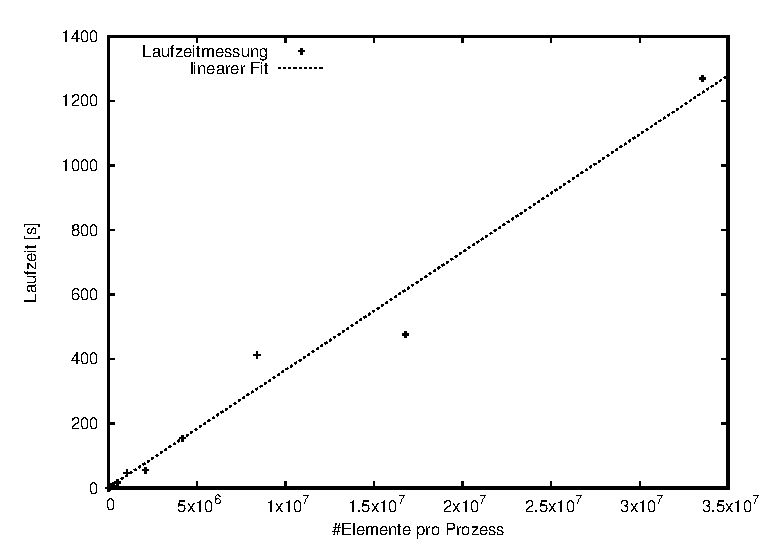
\includegraphics[width=0.8\textwidth]{img/grav1_lin.eps}
    \subcaption{Dieser Testlauf wurde mit $p = 1$ durchgeführt und entspricht damit der nicht-parallelen Variante.}
  \end{subfigure}
  \begin{subfigure}{\textwidth}
    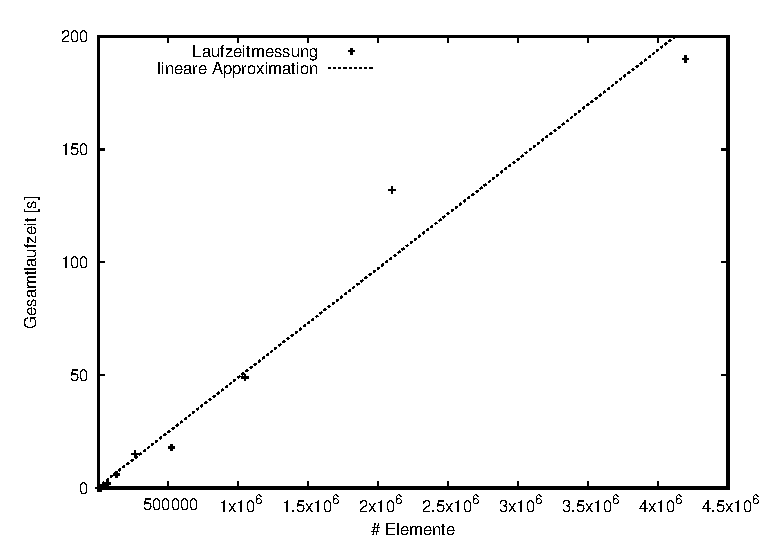
\includegraphics[width=0.8\textwidth]{img/grav_32_lin.eps}
    \subcaption{Dieser Testlauf wurde mit $p = 32$ durchgeführt, genau ein Knoten des Rechenclusters auszulasten.}
  \end{subfigure}
  \caption{In dieser Abbildung ist der Zusammenhang der Laufzeit mit der Anzahl an Elementen pro Prozess dargestellt.}
  \label{fig:1-32x}
\end{figure}
  \begin{table}[t]
 \begin{subtable}{0.45\textwidth}
  \begin{tabular}{c c c}
    \ \ \ \ 
    &
    \begin{tabular}{|P{2cm}|P{2cm}|}
      \hline
      \#Elemente \newline pro Prozess & Laufzeit [s] \\
      \hline
      $2^{10}$ & 0,008324 \\
      $2^{11}$ & 0,02569 \\
      $2^{12}$ & 0,04406 \\
      $2^{13}$ & 0,1348 \\
      $2^{14}$ & 0,503 \\
      $2^{15}$ & 0,6866 \\
      $2^{16}$ & 1,905 \\
      $2^{17}$ & 5,271 \\
      $2^{18}$ & 6,454 \\
      $2^{19}$ & 17,52 \\
      $2^{20}$ & 46,63 \\
      $2^{21}$ & 55,57 \\
      $2^{22}$ & 154,5 \\
      $2^{23}$ & 413,1 \\
      $2^{24}$ & 476 \\
      $2^{25}$ & 1270 \\
      \hline
    \end{tabular}
    &
    \ \ \ \ 
  \end{tabular}
 \subcaption{Dieser Testlauf wurde mit $p = 1$ durchgeführt und entspricht damit der nicht-parallelen Variante.}
 \end{subtable} \ \ 
 \begin{subtable}{0.45\textwidth}
  \begin{tabular}{c c c}
    \ \ \ \ 
    &
    \begin{tabular}{|P{2cm}|P{2cm}|}
      \hline
      \#Elemente \newline pro Pozess & Laufzeit [s] \\
      \hline
      $2^{10}$ & 0,02877 \\
      $2^{11}$ & 0,06701 \\
      $2^{12}$ & 0,1962 \\
      $2^{13}$ & 0,3097 \\
      $2^{14}$ & 0,7803 \\
      $2^{15}$ & 2,402 \\
      $2^{16}$ & 3,288 \\
      $2^{17}$ & 8,54 \\
      $2^{18}$ & 19,9 \\
      $2^{19}$ & 27,01 \\
      $2^{20}$ & 65,41 \\
      $2^{21}$ & 170 \\
      $2^{22}$ & 239,1 \\
      $2^{23}$ & 580,4\\
      & \\
      & \\
      \hline
    \end{tabular}
  \end{tabular}
 \subcaption{Dieser Testlauf wurde mit $p = 32$ durchgeführt, um genau ein Knoten des Rechenclusters auszulasten.}
 \end{subtable}
\caption{In dieser Tabelle sind die Laufzeitmessungen der ersten beiden Testläufe aufgeführt.}
\label{tab:1-32x}
\end{table}

  \begin{table}[b]
    \begin{tabular}{|l|c c c c c c c|}
%     \hline
%     $k_0$ & 1 & 2 & 3 & 4 & 5 & 6 & 7\\
    \hline
    $k$ & 1 & 8 & 27 & 64 & 125 & 216 & 343\\
    \hline
    Fehler\footnote{Ausführung mit einem Prozess. Entspricht der nicht-parallelisierten Variante} 
    & $2,66e^{-2}$ & $3,99e^{-3}$ & $5,26e^{-4}$ & $5,79e^{-5}$ & $5,14e^{-6}$ & $1,08e^{-6}$ & $1,96e^{-7}$\\
    \hline
    Fehler\footnote{Ausführung mit vier Prozessen, zum Überprüfen der Korrektheit der Parallelisierung.} 
    & $1,51e^{-2}$ & $2,25e^{-3}$ & $2,79e^{-4}$ & $3,09e^{-5}$ & $2,97e^{-6}$ & $5,66e^{-7}$ & $1,04e^{-7}$\\
    \hline
    Laufzeit [s] & 0,0486 & 0,0967 & 0,259 & 0,454 & 0,864 & 1,09 & 1,3\\
    \hline
    \end{tabular}
    \caption{Die Tabelle zeigt den Approximationsfehler des parallelen und nicht-parallelen Algorithmus in Abhängigkeit zur Anzahl Interpolationspunkte $k$.}
    \label{tab:error}
  \end{table}
  
  In den ersten beiden Testreihen wurde die Anzahl Sonnen pro Prozess bei konstanter Anzahl Prozesse variiert. Die Messergebnisse sind in \autoref{tab:1-32x} sowie in \autoref{fig:1-32x} 
  aufgeführt.
  
  Abbildung beziehungsweise Tabelle \textbf{(a)} bezieht sich jeweils auf die Testreihe mit einem Prozess, \textbf{(b)} auf die Testreihe mit 32 Prozessen. Trotz einiger Schwankungen, deren Herkunft
  nicht festgestellt werden konnte, ist der lineare Zuwachs gut zu erkennen. Bei der eingezeichneten Geraden handelt es sich um eine von gnuplot berechnete Regressionsgerade. Der Testlauf mit $32$ 
  Prozessen zeigt eine etwas stärkere Steigung, die vermutlich auf den erhöhten Kommunikationsaufwand zurückzuführen ist. Es sei auch angemerkt, dass bei gleicher Anzahl Elemente pro Prozess das
  Gesamtproblem $32$-Mal größer ist. Dennoch ist zu erkennen, dass die Approximation durch Interpolation und die Nutzung der $\mathcal{H}^2$-Struktur in beiden Fällen den theoretischen Berechnungen 
  auch in reellen Anwendungen gerecht wird und die Komplexität von $\mathcal{O}(n^2)$ auf $\mathcal{O}(k n)$ senken kann. Da $k$ wesentlich kleiner als $n$ ist, ist damit viel gewonnen.
  
  Um diese $\mathcal{H}^2$-Struktur nutzen zu können, hatten wir die eigentliche Kernfunktion durch Interpolation approximiert. Zwar haben wir über eine Zulässigkeitsbedingung sichergestellt, dass die 
  Ergebnisse ``vernünftig'' sind und Beweise angeführt, nach denen diese Approximation mit steigender Ordnung exponentiell gegen die eigentliche Kernfunktion konvergiert, aber wie ungenau wird die
  Berechnung durch die Approximation? 
  
  \TODO{Dazu wurden zwei Testreihen auf dem NEC-Cluster durchgeführt. Einmal wurde der Algorithmus mit nur einem Prozess ausgeführt, um eine nicht-parallel laufende Variante zu testen. Dazu wurde
  die Anzahl Elemente auf $n = 2^{16}$ gesetzt. Um die parallel arbeitende Variante vergleichen zu können wurde eine weitere Testreihe mit $p = 4$, $m = 2^{14}$ und damit $n = 4 \cdot m = 2^{16}$
  durchgeführt.}
  
  \TODO{Um zu ermitteln, welchen Fehler die Approximation induziert, wurde zunächst das Approximierte Simulationsergebnis berechnet. Anschließend wurden die Kräfte aller Sonnen durch den 
  nicht-approximierten vollbesetzten Algorithmus berechnet. Der Quotient der bedien Ergebnisse gibt dann die relative Abweichung des approximierten Algorithmus von der tatsächlichen Lösung an und ist
  in der Tabelle in den beiden ``Fehler''-Zeilen zu finden.}
  
  \TODO{Da es umständlich ist beide Testläufe mit exakt den selben Daten auszuführen, wurden jeweils getrennt die Abweichung von der korrekten Lösung berechnet. Somit lassen sich beide Testläufe
  indirekt vergleichen.}
  
  \TODO{Wie an den Daten zu erkennen ist, nimmt der Fehler bei jeder Erhöhung der Interpolationsordnung $k_0$ um einen Faktor zwischen $5$ und $10$ ab. Unsere Approximation konvergiert also in
  beiden Testläufen wie vorgesehen exponentiell. Allerdings fällt auf, dass die parallelisierte Variante fast durchgängig um etwa Faktor $2$ besser approximiert. Leider kann ich mir diese 
  Verbesserung nicht erklären und mir fehlte gegen Ende die Zeit diesem Phänomen auf den Grund zu gehen.}
  
  \subsubsection{Parallelität}
  \begin{figure}
  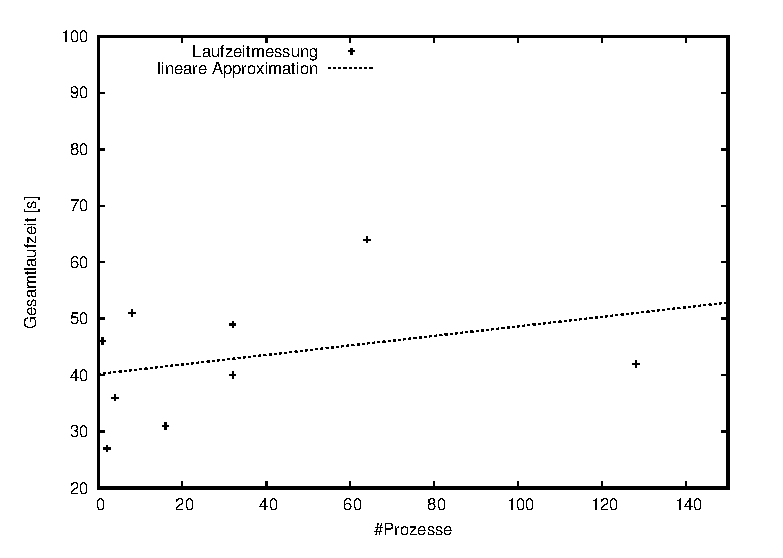
\includegraphics{img/grav_X20_lin.eps}
  \caption{Dieses Diagramm zeigt den Anstieg der Laufzeit in Abhängigkeit zur Anzahl Prozesse.}
  \label{fig:x20}
\end{figure}

\begin{table}[b]
  \begin{tabular}{|c|c|}
    \hline
    \#Prozesse & Laufzeit [s] \\
    \hline
    1 & 46,54 \\
    2 & 27,73 \\
    4 & 36,94 \\
    8 & 51,94 \\
    16 & 31,29 \\
    32\footnote{Die 32 Prozesse befanden sich auf einem Knoten des Clustersystems.} & 49,42 \\
    32\footnote{Die 32 Prozesse verteilten sich zu je 16 auf zwei Knoten des Clustersystems.} & 40,82 \\
    64 & 64,96 \\
    128 & 42,27 \\
    \hline
  \end{tabular}
  \caption{Tabelle der gemessenen Laufzeitdaten in Abhängigkeit zur Anzahl Prozesse.}
  \label{tab:x20}
\end{table}


  Bereits durch die höhere Steigung der Geraden in \autoref{fig:1-32x}.\textbf{(b)} gegenüber der in \textbf{(a)} lässt sich erahnen, dass durch die Kommunikation bei der Parallelisierung ein gewisser
  Overhead verursacht wird. Um dies genauer zu untersuchen, wurde die Anzahl Sonnen pro Prozess\footnote{Mit einer Verdoppelung der Prozessanzahl geht also auch eine Verdopplung der Anzahl Sonnen 
  einher.} auf $m = 2^{20}$ fixiert und die Anzahl Prozesse variiert.  Die Messdaten sind in \autoref{tab:x20} und \autoref{fig:x20} zu finden. 
  
  Die Daten unterliegen leider recht großen Schwankungen. Woher diese Schwankungen stammen, muss an anderer Stelle genauer untersucht werden, da es den Umfang und die Zielsetzung dieser Arbeit 
  übersteigt. Allerdings waren diese Ergebnisse in sich sehr stabil. Auch mehrfache Wiederholungen der einzelnen Testläufe haben immer bis auf wenige Zehntelsekunden dieselbe Zeit benötigt. 
  Trotzdem scheint mir, dass die errechnete Regressionsgerade die allgemeine Tendenz der Laufzeit einigermaßen akkurat wiedergibt.
  
  Ein gewisser Anstieg der Laufzeit ist zu erwarten, da der Kommunikationsaufwand steigt. Insgesamt zeigt sich aber die fast optimale Ausnutzung der Parallelität.
  
  Ein interessanter Effekt kann an den mit Fußnoten \textit{a} und \textit{b} gekennzeichneten Testläufen beobachtet werden. Während bei \textit{a} alle Prozesse auf einem Knoten gearbeitet haben, 
  wurden diese für den Testlauf \textit{b} auf zwei Knoten verteilt. Eine an sich naheliegende Vermutung wäre, dass die Testparameter für \textit{a} bessere Laufzeiten ergeben müssten,
  da die Kommunikation auf einem Rechner und ohne Netzwerkbeteiligung stattfinden kann. In der Realität hat sich aber gezeigt, dass es gerade umgekehrt ist. Vermutlich behindern sich die vielen 
  Speicherzugriffe bei dem Testlauf auf einem Knoten so stark, dass es effektiver ist einen Teil der Kommunikation über das Netzwerk zu führen. Auch dieser Effekt müsste gegebenenfalls an anderer Stelle 
  genauer untersucht werden.
  
  \clearpage
  
  \subsubsection{Speicherbedarf der Kommunikation}
  
  
%   Bei all den positiven Eigenschaften sei auch auf einen Nachteil des vorgestellten Algorithmus hingewiesen: Die verwendete Kommunikation benötigt viel unnötigen Speicher. Mein Hauptaugenmerk lag
%   darauf, die Kommunikation so einfach wie möglich zu gestalten, um die Laufzeit möglichst gering zu halten. Da die \code{MPI_Alltoallv(..)}-Methode exakt das benötigte Kommunikationsmuster liefert
%   und davon auszugehen ist, dass bei der Implementierung dieser Methode mehr Zeit und Know-How eingeflossen ist, als ich im Rahmen dieser Arbeit hätte investieren können, habe ich mich dazu entschieden
%   diese Methode zu nutzen. Die dafür notwendigen Puffer waren recht schnell konstruiert und wurden von mir zunächst nicht weiter beachtet. 
%   
%   Es hat sich aber gezeigt, dass bei 32 Prozessen auf einem Knoten mit $2^{22}$ Sonnen pro Prozess bereits $182$ GB Arbeitsspeicher benötigt werden. Das sind $5,68$ GB pro Prozess. Vergleicht man dies
%   mit dem Testlauf mit nur einem Prozess, der lediglich $52.37$ MB Hauptspeicher belegt, ist schnell einzusehen, dass die Kommunikation mit derart riesigem Pufferbedarf nicht tragbar ist.
%   \TODO{ausarbeiten!}
%   
%   Ganz ohne Puffer wird die Kommunikation nie auskommen. Es wäre aber möglich die Kommunikation durch nicht-blockierende Methoden derart zu verteilen, dass keinerlei Sendepuffer und lediglich 
%   Empfangspuffer für nicht-zulässige Blöcke benötigt würden. Dieser Ansatz ähnelt stärker dem von \citet{distrh2} vorgestellten Algorithmus, jedoch wäre weiterhin keine Kommunikation für Vorwärts- und 
%   Rückwärtstransformation notwendig. Eine genaue Ausarbeitung eines solchen Ansatzes muss leider aus Zeit- und Umfangsgründen an anderer Stelle fortgesetzt werden.
  
  

% \chapter{Verwandte Arbeiten}\label{chp:Related}
%   \blindtext

\chapter{Fazit und Ausblick}\label{chp:Conclusions}
  \section{Fazit}
    \blindtext
  \section{Ausblick}
    \blindtext

%%

\backmatter
  \tocbibliography

\end{document}
